% !TeX root = main.tex

\documentclass[openright,twoside,headsepline,bibliography=totoc]{scrbook}
% The document is a book with a few options:
%   openright: a new chapter is always on the right page
%   twoside: left and right margins are inverted for even and odd pages

% == Packages and some options
\usepackage{amssymb,amsmath}
\usepackage{ifxetex,ifluatex}
\usepackage{fix-cm}
\usepackage{microtype}  % better justifications, amongst others
\usepackage{longtable,booktabs}

% Make hyperref silent, it's always complaining for tokens like \beta
\usepackage{silence}
%\WarningFilter*{hyperref}{Token not allowed in a PDF string (Unicode)}

\usepackage[unicode=true,pdfa]{hyperref}
\hypersetup{breaklinks=true,
            pdfauthor={Maël Le Garrec},
            pdftitle={LHC Effective Model for Optics Corrections},
            colorlinks=true,
            citecolor=blue,
            urlcolor=blue,
            linkcolor=black,
            pdfborder={0 0 0}}
\usepackage[capitalise]{cleveref}
\usepackage[english]{babel}

% == FONTS
\usepackage{calligra}  % font for quote page
%\usepackage{libertinust1math}
\usepackage{libertine}  % font for the whole document
\usepackage[libertine]{newtxmath}
%\usepackage{lmodern}  % font based on Computer Modern for the whole doc
% ==


\usepackage{wasysym}
\usepackage{enumitem}  % to define new lists
\usepackage{tikz}  % for drawing figures by code
\usepackage{siunitx}
\usepackage{graphicx}
\usepackage{caption}
\usepackage{ragged2e}
\usepackage{atveryend}
%\usepackage{subfigure} (???)
\usepackage{subcaption}
\usepackage{pgf}  % fileformat for the flipbook
\usepackage{xcolor,soul}
\usepackage{lscape}  % landscape
\usepackage{changepage}
\usepackage[nonumberlist,acronyms,nogroupskip]{glossaries}
\usepackage{glossary-longbooktabs}
\usepackage{setspace}
\usepackage[english]{babel}
\usepackage{float}
%\usepackage[subfigure]{tocloft}
\usepackage{titletoc}
\usepackage{etoc}  % local tables of content
\usepackage{imakeidx}
\usepackage{lipsum}
\usepackage{geometry}
\usepackage[automark]{scrlayer-scrpage} % for headers and footers
\usepackage{scrhack}  % to remove some warnings
\usepackage{blindtext}
%\usepackage{unicode-math} % Setup an unicode font for regular typing and for maths  // clashes with OverBrace from nicematrix
\usepackage{amsmath}
\usepackage{mathtools}  % for some functions, like DeclarePairedDelimiter
\usepackage{svg}
\usepackage{nicematrix}
\usepackage[
  height={2cm},
  topthumbmargin={auto},
  bottomthumbmargin={auto},
  eventxtindent={4mm},
  oddtxtexdent={2.5mm}]{thumbs}  % markers on the side to show the chapter
\usepackage[%
  backend=bibtex        % biber or bibtex
%,style=authoryear      % Alphabeticalsch
 ,style=numeric-comp    % numerical-compressed
 ,sorting=none          % no sorting
 ,sortcites=true        % some other example options ...
 ,block=none
 ,indexing=false
 ,citereset=none
 ,isbn=false
 ,url=true
 ,doi=true              % prints doi
 ,natbib=true           % if you need natbib functions
]{biblatex}
\AtEveryBibitem{%  % in the bibliography
    \clearlist{language}%  % remove language from citations
    \clearfield{urlyear}%  % to remove the "visited on"
    \clearfield{urlmonth}%
    \clearfield{urlday}%
    \clearfield{day}%  % only print the year
    \clearfield{month}%
    \clearfield{endday}%
    \clearfield{endmonth}%
    \clearfield{note}%  % information about the PDF, like size and number of pages
    \clearfield{pages}%  % which pages in the book
}
\AtEveryCitekey{%  % for \fullcite
    \clearlist{language}%
    \clearfield{urlyear}%
    \clearfield{urlmonth}%
    \clearfield{day}%
    \clearfield{month}%
    \clearfield{endday}%
    \clearfield{endmonth}%
    \clearfield{note}%
    \clearfield{pages}%
}
\addbibresource{library.bib}  % better than \bibliography
\usepackage{csquotes}  % Changes the quotestyle depending on the language, useful for bibliography

% Flipbook
\usepackage{flipbook}
\cfoot*{
  \flipbookframe[1][1]{../flipbook/frames/frame_}[pgf][0.2]
  % start frame
  % speed of the animation per page
  % scale
}


% To have big numbers at the start of each chapter
%\definecolor{gray75}{gray}{0.75}
%\newcommand{\hsp}{\hspace{0pt}}
%\titleformat{\chapter}[hang]
%    {\flushright\fontseries{b}\fontsize{80}{100}\selectfont}
%    {\fontseries{b}\fontsize{100}{130}\selectfont \textcolor{gray75}\thechapter\hsp}
%    {0pt}
%    {\\ \Huge\bfseries}[]
%
%% Same but un-numbered
%\titleformat{name=\chapter, numberless}[hang]
%    {\flushright\fontseries{b}\fontsize{80}{100}\selectfont}
%    {\fontseries{b}\fontsize{100}{130}\selectfont \textcolor{gray75}\hsp}
%    {0pt}
%{\\ \Huge\bfseries}[]
%
%% And now the other titles
%\titleformat{\section}
%{\normalfont\Large\bfseries}{\thesection}{1em}{}
%\titleformat{\subsection}
%{\normalfont\large\bfseries}{\thesubsection}{1em}{}
%\titleformat{\subsubsection}
%{\normalfont\normalsize\bfseries}{\thesubsubsection}{1em}{}
%\titleformat{\paragraph}[runin]
%{\normalfont\normalsize\bfseries}{\theparagraph}{1em}{}
%\titleformat{\subparagraph}[runin]
%{\normalfont\normalsize\bfseries}{\thesubparagraph}{1em}{}



% ===========================================================================
%                            SOME OPTIONS
% ===========================================================================

% Set the geometry of the pages
% For a twoside book like this one, `left` and `right` mean respectively `inner` and `outer`
% The numbers are based on the "Canon des Ateliers", https://etnadji.fr/rsc/canon/calcul.php
% tête = top, pied = bottom, petit fond = left, grand fond = right
%\geometry{a4paper, top=2.625cm, left=2.1cm, right=3.15cm, bottom=3.675cm, includehead, includefoot}
\geometry{b5paper, top=2.2cm, left=1.76cm, right=2.64cm, bottom=3.08cm, includehead, includefoot} % courant
%\geometry{b5paper, top=2.935cm, left=2.348cm, right=3.522cm, bottom=4.109cm, includehead, includefoot} % luxe

% Vertical space before chapters
\RedeclareSectionCommand[beforeskip=5pt,
afterskip=2cm]{chapter}

% Fancy chapter headings, needs to be loaded after geometry
%\usepackage[Bjornstrup]{fncychap}  % issues a lot of warnings with scrbook, replaced in commands below

% Factor spacing between lines
\linespread{1.1}

\numberwithin{equation}{chapter}
\numberwithin{table}{chapter}
\numberwithin{figure}{chapter}
\newcommand*\diff{\mathop{}\!\mathrm{d}}

% Set some lengths
\setlength{\parindent}{12pt}
\setlength{\parskip}{6pt plus 2pt minus 1pt}
\setlength{\emergencystretch}{3em}  % prevent overfull lines
\setcounter{secnumdepth}{2}  %  set up to which point a sub[..]subsection is numbered

\urlstyle{same}  % don't use monospace font for urls

% Make the captions closer to table, figures, etC.
%\setlength{\belowcaptionskip}{-5pt}
%\setlength{\abovecaptionskip}{-5pt}

% Define some colors
\definecolor{thumb_color}{HTML}{D9D9D9}

% LaTeX will stretch the page to fit vertically on the whole page as part of the "book" style
% This prevents it
%\raggedbottom

% ===========================================================================
%                            SOME COMMANDS
% ===========================================================================

% Create a \tightlight command for itemize environments to have the bullet points closer together
\providecommand{\tightlist}{%
  \setlength{\itemsep}{0pt}\setlength{\parskip}{0pt}}

% Command to create highlights easily in colors
\DeclareRobustCommand{\hlcyan}[1]{{\sethlcolor{cyan}\hl{#1}}}

% Display a table of contents for the current chapter
\newcommand{\chaptertoc}[1][Contents]{%
  % Set the indent so it's a bit tighter and looks better
  %\setlength{\cftsecindent}{0.2cm}
  %\setlength{\cftsubsecindent}{0.8cm}
  %\setlength{\cftsubsubsecindent}{1.4cm}

  %\etocmulticolstyle{\addsec*{#1\\\rule{\textwidth}{0.4pt}}}%
  \setcounter{tocdepth}{3}

  % Reduce the spacing between the list items
  %\addsec*{\rule{\textwidth}{0.4pt}}
  \begin{spacing}{0.1}
    \localtableofcontents%
  \end{spacing}
}

% Define a wrapper for \addthumb, to add markers on the side
\newcommand{\thumbforchapter}{\addthumb{Chapter \thechapter}{\Large{\thechapter}}{black}{thumb_color}}
% Same but with letters for the appendices
\newcommand{\thumbforappendix}{\addthumb{Chapter \thechapter}{\Large{\thechapter}}{black}{thumb_color}}

% When using align from amsmath, each line is numbered
% This allows to use align* and the manually number the last equation
\newcommand\numberthis{\addtocounter{equation}{1}\tag{\theequation}}

% Some commands to display text in color
% To do in red
\newcommand*{\todo}[1]{{\bfseries\color{red}#1}}
% To be reviewed in orange
\newcommand*{\review}[1]{{\bfseries\color{orange}#1}}
% OK in green
\newcommand*{\done}[1]{{\bfseries\color{green}#1}}


% For commands floor and ceil to be easier to type
\DeclarePairedDelimiter\ceil{\lceil}{\rceil}
\DeclarePairedDelimiter\floor{\lfloor}{\rfloor}



% Nice looking chapters
\renewcommand*{\chapterformat}{\thechapter}
\renewcommand*{\raggedchapter}{\raggedleft}
\setkomafont{chapter}{\LARGE}
\setkomafont{chapterprefix}{\Huge}
\newcommand*{\ChapterCase}[1]{#1}
%\newcommand*{\ChapterCase}[1]{\MakeUppercase{#1}}%  ugly
%\newcommand*{\ChapterCase}[1]{\MakeUppercase{\textls[75]{#1}}}% better
\newsavebox\chapternumberbox
\renewcommand*{\chapterlinesformat}[3]{% #1 = chapter command name
                                       % #2 = number (or empty)
                                       % #3 = text
  \rule[-\dp\strutbox]{\linewidth}{.4pt}%
  \sbox\chapternumberbox
  {%
    \makebox[0pt][l]{%
      \hspace{-\linewidth}\hspace{.5em}%
      \colorbox{black}{%
        \parbox[c][1.5em][c]{1.5em}{%
          \centering
          \textcolor{white}{%
            \usekomafont{chapterprefix}{%
              \strut #2%
            }%
          }%
          \par
        }%
      }%
    }%
  }%
  \IfArgIsEmpty{#2}{%
    \vphantom{\usebox\chapternumberbox}%
  }{\usebox\chapternumberbox}%
  \par
  \ChapterCase{\strut\ignorespaces #3}%
  \rule[.5em]{\linewidth}{.4pt}\par
}

% Glossary stuff
% === Define the different glossaries
\newglossary*{nomenclature}{Nomenclature}
\newglossary*{symbols}{Symbols}

\makeglossaries

% === Add the different entries
\newglossaryentry{Dipole}{type=nomenclature,name=Dipole, description={ Magnets with two poles, responsible for bending the particles in the accelerator. }}
\newglossaryentry{LBDS}{type=nomenclature,name=LBDS, description={LHC Beam Dump System }}
\newglossaryentry{Crosstalk}{type=nomenclature,name=Crosstalk, description={Interferences between two electronic circuits }}
\newglossaryentry{Laundau Octupole}{type=nomenclature,name=Laundau Octupole, description={Octupoles that introduce a spread in the beam, making it more stable }}
\newglossaryentry{BPM}{type=nomenclature,name=BPM, description={ Beam Position Monitor, gives the transverse position of the beam }}
\newglossaryentry{DOROS}{type=nomenclature,name=DOROS, description={ Low noise BPM. Currently can't be used with other BPMs due to synchronization issues  }}
\newglossaryentry{Dispersion}{type=nomenclature,name=Dispersion, description={ Change of orbit with momentum offset, mainly in the horizontal plane, created by the dipoles}}
\newglossaryentry{Coupling}{
    type=nomenclature,
    name=Coupling,
    description={ 
        Correlation between the motion of particles in horizontal or vertical plane to the other.
        Strong coupling negatively impacts the optics and is usually avoided. 
    }
}
\newglossaryentry{Emittance}{type=nomenclature,name=Emittance, description={ (\ensuremath{\epsilon}) Unit describing the beam in phase space. A low emittance indicates a beam with a small momentum offset and confined to a small distance }}
\newglossaryentry{beta-function}{
    type=nomenclature,
    name=Beta-function, 
    description={
        Variable of the twiss-parameters: $\beta$ as a function of the longitudinal position $s$.
        Related to the transverse beam size: $\sigma(s)= \sqrt{\epsilon \cdot \beta(s)}$ 
    }
}
\newglossaryentry{Chromaticity}{type=nomenclature,name=Chromaticity, description={ Tune change with momentum offset. Usually denoted as three orders: $Q'$, $Q''$ and $Q'''$ }}
\newglossaryentry{Aperture}{type=nomenclature,name=Aperture, description={ Maximum physical transverse size the beam can take in the accelerator without suffering losses }}
\newglossaryentry{Dynamic Aperture}{type=nomenclature,name=Dynamic Aperture, description={ Maximum stable aperture. Above that size, the particles become unstable and become lost }}
\newglossaryentry{Waist}{type=nomenclature,name=Waist, description={ Location where the $\beta$-function is at is minimum in an IP. $\beta^*$ refers to $\beta_{waist}$ }}
\newglossaryentry{Waist Shift}{type=nomenclature,name=Waist Shift, description={ Changing the waist to have $\beta^* = \beta_{IP}$ }}
\newglossaryentry{Rigid Waist Shift}{type=nomenclature,name=Rigid Waist Shift, description={ Doing a waist shift by powering all the triplets at once. No individual trim }}
\newglossaryentry{Orbit Feedback}{type=nomenclature,name=Orbit Feedback, description={ System responsible for acquisition and correction of the orbit }}
\newglossaryentry{ATS Factor}{type=nomenclature,name=ATS Factor, description={ Equivalent to the ratio of the virgin $\beta$-function to the $\beta$-function used in the current ATS scheme, at the edge of the arc  }}
\newglossaryentry{AC-Dipole}{
    type=nomenclature,
    name=AC-Dipole,
    description={
        Dipole magnet generating a variable oscillating field. Used to force beam oscillations for
        optics measurements.
    }
}


% ==== Acronyms
\newacronym{lhc}{LHC}{Large Hadron Collider}


% ==== Symbols
\newglossaryentry{action}
{
    type=symbols,
    name=action,
    symbol=$\mathcal{J}$,
    description={Action used as coordinate blabla},
}


% ===========================================================================

\begin{document}

% stfu hyperref
\WarningFilter{hyperref}{Token not allowed in a PDF string}


% =================================================
%           Stuff at the very beginning
% =================================================
\frontmatter  % use roman numerals here for pages
% ===============================================================
%                         MAIN PAGES
% ===============================================================

% This file contains several pages
% The first one is the very first page of the thesis, containing the name and author
% The second page contains the information about the supervisors and the university


% =================================
%           Main Title
% =================================
\begin{titlepage}
    \makeatletter
    \def\subtitle#1{\def\@subtitle{#1}}
    \def\maketitle{%
        % Redefine the geometry of the page
        % That's the same of the rest of the document, without the includehead and footer
        % Right and left are also the same
        %\newgeometry{top=20.625mm, bottom=28.875mm, left=16.5mm, right=16.5mm}
        \thispagestyle{empty} % remove numbering
        % 3 lines
        \noindent\rule[0.5em]{\textwidth}{1.5pt}\vspace{-22pt}
        \noindent\rule[0.5em]{\textwidth}{1.5pt}\vspace{-22pt}
        \noindent\rule[0.5em]{\textwidth}{1.5pt}
        \vspace{0.5cm}
        % Title
        \chapterfont\fontsize{33pt}{30pt}\selectfont%
        \begin{flushright}%
            \bfseries
            \MakeUppercase{
                \@title
            }%
        \end{flushright}
        % Small text
        \vspace{.1em}
        \subtitlefont\fontsize{11pt}{15pt}\selectfont%
        \begin{flushright}%
            \@subtitle
        \end{flushright}
        % Big vertical space
        \vfill
        % Author
        \chapterfont\fontsize{15pt}{0pt}\selectfont%
        \bfseries\noindent\scshape\@author
        % 2 rules
        \par
        \vspace{0.7em}
        \noindent\rule[0.5em]{\textwidth}{1.5pt}\vspace{-20pt}
        \noindent\rule[0.5em]{\textwidth}{1.5pt}
    }
    \makeatother
    
    \title{LHC Effective Model for Optics Corrections}
    \subtitle{Measurements and corrections of high-order non-linear optics}
    \author{Maël Le Garrec}
    
    \clearpage\maketitle
    \restoregeometry
\end{titlepage}




% =================================
%         Secondary Page
% =================================
% With german specific terms etc.
% Sizes for B5: 11pt/12pt
% 0.9cm / 0.4cm * 3
{
    \makeatletter
    \def\subtitle#1{\def\@subtitle{#1}}
    \def\firstsupervisor#1{\def\@firstsupervisor{#1}}
    \def\secondsupervisor#1{\def\@secondsupervisor{#1}}
    \def\makesecondtitle{%
        \thispagestyle{empty} % remove numbering
        % 3 lines
        \noindent\rule[0.5em]{\textwidth}{1.5pt}\vspace{-22pt}
        \noindent\rule[0.5em]{\textwidth}{1.5pt}\vspace{-22pt}
        \noindent\rule[0.5em]{\textwidth}{1.5pt}
        % Title
        \chapterfont\fontsize{27pt}{27pt}\selectfont%
        \begin{center}%
            \bfseries
            \MakeUppercase{
                \@title
            }
        \end{center}
        \vspace{1.3cm}
        % Back to normal font for the German specific text
        \normalfont\subtitlefont\fontsize{11pt}{15pt}\selectfont%
        \center{
            Dissertation \\ 
            zur Erlangung des Doktorgrades \\
            der Naturwissenschaften
        }
        \vspace{0.8cm}
        \center{
            Vorgelegt beim Fachbereich Physik \\
            der Johann Wolfgang Goethe-Universität \\
            in Frankfurt am Main
        }
        \vspace{0.8cm}
        \center{
            von \\
            \scshape{Maël Le Garrec}\normalfont\subtitlefont\fontsize{11pt}{15pt}\selectfont\\
            aus Oberhaslach, Elsàss, Frankreich.
        }
        \vspace{0.8cm}
        \center{
            Unter der Betreuung von\\
            Dr. Ewen H. Maclean, CERN,\\
            Apl. Prof. Dr. Giuliano Franchetti, Goethe-Universität.
        }
        %
        % Supervisors
        %\center{
        %    \@firstsupervisor \\
        %    \@secondsupervisor
        %}
        %
        \vfill
        \begin{center}
            Frankfurt am Main 2024
        \end{center}
    }
    \makeatother
    
    \title{LHC Effective Model for\\Optics Corrections}
    \subtitle{Measurements and corrections of high-order non-linear optics}
    \firstsupervisor{Dr. Ewen H. Maclean}
    \secondsupervisor{Apl. Prof. Dr. Giuliano Franchetti}
    \author{Maël Le Garrec}

    % Force page to be odd
    \cleardoublepage
    % Display the second title page
    \makesecondtitle
}


% =================================
%            Third Page
% =================================
% With signatures
{
    \makeatletter
    \def\makethirdtitle{%
        \thispagestyle{empty} % remove numbering
        \normalfont\subtitlefont\fontsize{11pt}{15pt}\selectfont%
        
        \begin{flushleft}
            Vom Fachbereich Physik der Johann Wolfgang Goethe-Universität als Dissertation angenommen.
        \end{flushleft}
        \vspace{7cm}

        \noindent Dekan:

        \vspace{4cm}
        \noindent Gutachter:

        \vspace{4cm}
        \noindent Datum der Disputation:
    }
    \makeatother
    
    % Force page to be even
    \clearpage
    % Display the second title page
    \makethirdtitle
}
\chapter*{ToDo List}

\begin{itemize}
    \tightlist
    \item Change \verb|\cref| for \verb|\Cref| at the beginning of sentences.
    \item Change tocdepth to 2
\end{itemize}  % That's just a todo list basically
\chapter{\review{Abstract}}

% That's so the extended summary does not feel too weird
\ifthenelse{\equal{\papersize}{A4}}{ % A4
    \newcommand{\fontsizeabstract}{12pt}
    \newcommand{\fontskipabstract}{14pt}
}{  % else, B5
    \newcommand{\fontsizeabstract}{11pt}
    \newcommand{\fontskipabstract}{11pt}

    \vspace{-0.5cm}
}

{
\fontsize{\fontsizeabstract}{\fontskipabstract}\selectfont

This thesis investigates the crucial role of higher-order magnetic fields and non-linear optics in
the stability and performance of particle accelerators, focusing on the Large Hadron Collider (LHC)
at CERN. The control of non-linear optics, which deals with the interaction of charged particle 
beams with complex magnetic fields such as sextupolar, octupolar, decapolar, and so on, is essential
for managing beam dynamics. The LHC, as the world's most powerful accelerator, provides a unique
opportunity to study these high-order effects, serving as a testbed for future accelerator designs.

These higher-order fields significantly affect the beam's dynamic aperture and lifetime, especially
at injection energy, where precise correction of magnetic field errors is required. Managing these
challenges is not only vital for optimizing LHC performance but also for guiding the design and
operation of next-generation machines.

A key contribution of this work is the development of correction methods for Resonance Driving Terms
(RDTs), a critical factor in beam lifetime and dynamic aperture limitations. New corrective
strategies for RDTs have led to notable improvements in beam lifetime and dynamic aperture at both
injection and top energy operation. This thesis also addresses the discrepancies observed between
experimental measurements and models of beam observables.

These findings highlight the importance of precise modeling and correction of non-linear magnetic
fields, offering insights that will benefit both the LHC and future high-energy particle
accelerators.
}
\include{chapters/00_Preamble/03_zusammenfassung}


% =================================================
%               Acknowledgements
% =================================================
% ===========================================================================
%                  Acknowledgements
% ===========================================================================
\chapter{\todo{Acknowledgements}}  % Have the chapter un-numbered, but still showing up in the contents


Rogelio
Michael Hoffer
Joschua Dilly
Félix Soubelet
Félix Carlier 
Sébastien Joly
Ewen
Leon 
Jacqueline
Jack
Michi Hostettler
David
Josephine
Andreas
Elena
Dora
Joanna


JB Potoine
Vittorio
Wietse
Bjorn
Frank Zimmerman
Christian

Christophe
Roxana Soos 
Sofia

IRC
\clearpage

\thispagestyle{empty}
\null\vfill

\newlength\longest
\settowidth\longest{\huge\itshape Check Yourself before you Shrek yourself blabla;}
\parbox{\longest}{%
  \centering
  \raggedright{\huge\itshape%
  \calligra Check yourself before you Shrek yourself.\par\bigskip
  }
  \raggedleft\large\MakeUppercase{Ice Cube ft. Shrek}\par%
}

\vfill\vfill

\clearpage



% =================================================
%               Table of Contents
% =================================================
\setcounter{tocdepth}{2}  % set it back to 2 for the final version
%\setcounter{tocdepth}{5}
%\cleardoublepage
%\addcontentsline{toc}{chapter}{Contents}
\tableofcontents


% =================================================
%                    Glossary
% =================================================
\chapter{\review{Glossary}}
\label{glossary}

\renewcommand{\glossarysection}[2][]{}
\renewcommand{\glsnamefont}[1]{\chapterfont\small\textbf{#1}}
%\setglossarystyle{tree}
\glsnoexpandfields  % fixes any issues with commands inside definitions


% === Definitions
\section*{Nomenclature}\label{equipment}
\vspace{-20pt}
\glsaddall[types={nomenclature}]
\printglossary[type=nomenclature, style=list]


% === Acronyms
\section*{Acronyms}\label{acronyms}
\vspace{-20pt}
\glsaddall
\glssetwidest{MAD-X\_}  % widest acronym (plus _) so everything is aligned
\printglossary[type=\acronymtype,style=alttree]


% === Symbols
\section*{Symbols}\label{symbols}
\vspace{-20pt}
\glsaddall
\glssetwidest{AAAA}
\printglossary[type=symbols, style=alttree]


\newpage


% =================================================
%                    Chapters
% =================================================
\mainmatter  % back to arabic numbers
%\chapter{Theory}
\thumbforchapter{}
\chaptertoc{}

\section{Units}\label{units}

\begin{itemize}
\item
  Joules: \[1 J = 1 N \cdot m = 1 kg \cdot m^2 \cdot s^{-2}\]
\item
  Electronvolt:

  \begin{itemize}
  \tightlist
  \item
    \(eV = e \cdot V\)

    \begin{itemize}
    \tightlist
    \item
      e: elementary charge
    \item
      V: volt
    \end{itemize}
  \item
    \(1 eV = 1.602176634 \cdot 10^{-19} J\)
  \end{itemize}
\item
  Momentum:

  \begin{itemize}
  \tightlist
  \item
    \(p\) in \(kg.m.s^{-1}\)
  \item
    \(p\) in \(eV.c^{-1}\): \(J \cdot c^{-1} = kg.m.s^{-1}\)
  \end{itemize}
\item
  Tesla \[T = \frac{V \cdot s}{m}\]
\end{itemize}

\newpage

\hypertarget{definitions}{%
\section{Definitions}\label{definitions}}

\hypertarget{some-math-definitions}{%
\subsection{Some Math Definitions}\label{some-math-definitions}}

\begin{itemize}
\item
  Harmonic Oscillator \[F = -kx\] \[x'' = -\frac{k}{m}x \]
\item
  Magnetic rigidity, used for dipoles: \[B\rho = \frac{p}{q}\]

  \begin{itemize}
  \item
    B: magnetic field {[}\(T\){]}
  \item
    \(\rho\): radius of curvature of the orbit {[}\(m\){]}
  \item
    p: momentum {[}\(eV/c\){]}
  \item
    q: particle charge {[}\(e\){]}
  \item
    Can be expressed as \[B \rho = 3.3356 p\] if \(p\) is in GeV/c
  \end{itemize}
\item
  Magnets orders
\end{itemize}

\begin{center}
  \begin{tabular}{lllllll}
  Magnet Letter          & B & Q & S & O & D & T \\
  Number of Poles        & 2 & 4 & 6 & 8 & 10 & 12 \\
  a (skew) designation   & 1 & 2 & 3 & 4 & 5 & 6 \\
  b (normal) designation & 1 & 2 & 3 & 4 & 5 & 6 \\
  K designation          & 1 & 2 & 3 & 4 & 5 & 6 \\
  MADX-K                 & 0 & 1 & 2 & 3 & 4 & 5 \\
  \end{tabular}
\end{center}

\begin{itemize}
\item
  Magnet Strength:
  \begin{equation}K_{n} = \frac{q}{P} (n-1)!B_n\label{eq:magnet_strength}\end{equation}

  \begin{itemize}
  \item
    The unit is given by:

    \begin{itemize}
    \tightlist
    \item
      k1: dipole: \(m^{-1}\)
    \item
      k2: quadrupole: \(m^{-2}\)
    \item
      k3: sextupole: \(m^{-3}\)
    \item
      k4: octupole: \(m^{-4}\)
    \item
      k5: decapole: \(m^{-5}\)
    \item
      k6: dodecapole: \(m^{-6}\)
    \end{itemize}
  \item
    If interested in the \emph{integrated} strength, multiply by
    \emph{m}
  \end{itemize}
\item
  Dispersion is given via:
  \begin{equation}D = \frac{\Delta x}{\delta}\end{equation}
\item
  The relative momentum offset is defined via the reference momentum and
  the momentum
  \begin{equation}\delta = \frac{\Delta P}{P_0} = \frac{P - P_0}{P_0}\label{eq:dpp}\end{equation}
\item
  Relation between the action and the single particle emittance:
  \href{https://journals.aps.org/prab/pdf/10.1103/PhysRevSTAB.17.081002}{Non
  Linear Observables} (eq. 2):
  \begin{equation}2J_{x,y} = \epsilon_{x,y}\end{equation}
\item
  The tune is defined as the derivative of the Hamiltonian relative to
  the action.
  \begin{equation}Q_{x,y} = \frac{\partial \left< H \right>}{\partial J_{x,y}}\end{equation}
\item
  The tune can also be defined as:
  \begin{equation}Q_{x,y} = \frac{1}{2 \pi} \oint \frac{1}{\beta_{x,y}(s)} \,ds\end{equation}
\item
  The phase advance in the \(x\) plane, between two elements \(w\) and
  \(j\), in the accelerator is given by
  \href{https://arxiv.org/abs/1711.06589}{AnalyticFormulasFranchi}:
\end{itemize}

\begin{equation}
\begin{cases} 
  \Delta \phi_{x,wj} = \left(\phi_{x,j} - \phi_{x,w} \right)              & \mbox{if } \phi_{x,j} > \phi_{x,w}, \\
  \Delta \phi_{x,wj} = \left(\phi_{x,j} - \phi_{x,w} \right) + 2 \pi Q_x  & \mbox{if } \phi_{x,j} < \phi_{x,w}.
\end{cases}
\end{equation}

\newpage

\hypertarget{maths}{%
\section{Maths}\label{maths}}

\hypertarget{taylor-series}{%
\subsection{Taylor Series}\label{taylor-series}}

The Taylor series of a multivariable function at the point
\((a_1, \cdots, a_d)\) is defined as:

\begin{equation}\begin{aligned}
  f(x_1, \cdots, x_d) = &f(a_1, \cdots, a_d) \\
                &+ \frac{1}{1!} \sum_{j=1}^{d} \frac{\partial f(a_1, \cdots, a_d)}{\partial x_j} (x_j - a_j) \\
                &+ \frac{1}{2!}\sum_{j=1}^{d}\sum_{k=1}^{d} \frac{\partial^2 f(a_1, \cdots, a_d)}{\partial x_j\partial x_k} (x_j - a_j) (x_k - a_k) \\
                &+ \frac{1}{3!}\sum_{j=1}^{d}\sum_{k=1}^{d}\sum_{l=1}^{d} \frac{\partial^3 f(a_1, \cdots, a_d)}{\partial x_j\partial x_k\partial x_l} (x_j - a_j) (x_k - a_k) (x_l - a_l)\\
                &+ \cdots
\end{aligned}\label{eq:taylor}\end{equation}

\hypertarget{non-linear-transfer-maps}{%
\subsection{Non-Linear Transfer Maps}\label{non-linear-transfer-maps}}

For linear dynamics, linear transfer maps can be used to describe a
particle's position from the elements in the lattice and the particle's
current position. In the non linear case, such a formalism can't be
used. Instead, the Lie operator is used.

\hypertarget{lie-operator}{%
\subsubsection{Lie Operator}\label{lie-operator}}

Resources found in
\href{https://mlegarre.web.cern.ch/mlegarre/Courses/Meghan_RDTpresentation.pdf}{Meghan
McAteer's talk} and Wolski's book.

The Lie operator is defined as:

\[
\colon f \colon = \sum^n_{i=1} \left(\frac{\partial f}{\partial x_i} \frac{\partial}{\partial p_i} 
                           - \frac{\partial f}{\partial p_i} \frac{\partial}{\partial x_i}
                      \right)
\]

With \emph{i} the index of a dimension. So \(x_1\) would be \(x\) and
\(x_2\), \(y\).

The exponential Lie operator \(e^{:f:}\) acting on a function \(g\):

\begin{equation}e^{:f:}g = g + [f, g] + \frac{1}{2} [f, [f, g]] + \cdots\label{eq:Lie}\end{equation}

This is from the usual power series of an exponential:

\[e^{:f:} = \sum^{\infty}_{m=0} \frac{:f:^m}{m!}\]

Where \([f, g]\) is a poisson bracket, still somehow used for historical
reasons:

\begin{equation}[f, g] = \colon f \colon g
\label{eq:poisson_bracket}\end{equation}

Thus, the particle with coordinates \(\vec{x}\) passing through an
element can be mapped using the Hamiltonian of the element (Wolski, eq.
9.6):

\begin{equation}\vec{x}_f = e^{-\Delta s:H:} \vec{x}_0\label{eq:position_non_linear}\end{equation}

For a \emph{thin} lens, we can directly multiply by the length of the
magnet:

\begin{equation}\vec{x}_f = e^{-L:H:} \vec{x}_0\label{eq:position_non_linear_thin}\end{equation}

By combining \cref{eq:Lie} and \cref{eq:position_non_linear}, we obtain:

\begin{equation}
\begin{aligned}
\left[H, \vec{x}_0\right] =& \frac{\partial H}{\partial x} \frac{\partial \vec{x}_0}{\partial p_x} 
                                    -\frac{\partial H}{\partial p_x} \frac{\partial \vec{x}_0}{\partial x} \\
                           &\frac{\partial H}{\partial y} \frac{\partial \vec{x}_0}{\partial p_y} 
                                    -\frac{\partial H}{\partial p_y} \frac{\partial \vec{x}_0}{\partial y}
\end{aligned}
\label{eq:bracket_hamiltonian}\end{equation}

Thus giving us the complete equation:

\begin{equation}
\begin{aligned}
\vec{x}_f &= e^{:H:}\vec{x}_0 \\
          &= \vec{x}_0 + \left[H, \vec{x}_0\right] \\
          &= \begin{pmatrix} x \\ p_x \\ y \\ p_y\end{pmatrix}_0
             + \begin{pmatrix} -\frac{\partial H}{\partial p_x} \\ 
                               \frac{\partial H}{\partial x} \\
                               -\frac{\partial H}{\partial p_y} \\
                               \frac{\partial H}{\partial y}
               \end{pmatrix} \\
\begin{pmatrix} x \\ 
                p_{x} \\
                y \\
                p_{y} 
\end{pmatrix}_f
          &=  \begin{pmatrix} x_0 - \dfrac{\partial H}{\partial p_x} \\ 
                               p_{x0} +\dfrac{\partial H}{\partial x} \\
                               y_0 - \dfrac{\partial H}{\partial p_y} \\
                               p_{y0} +\dfrac{\partial H}{\partial y}
               \end{pmatrix}
\end{aligned}
\label{eq:non_linear_map}\end{equation}

This non linear transfer map is a general map without coupling.

\hypertarget{multipole-expansion}{%
\subsection{Multipole Expansion}\label{multipole-expansion}}

This is the Hamiltonian for a magnetic element with normal strength
component \emph{K} and skew component \emph{J}:

\begin{equation}H = \Re \left[\sum_{n>1} \left( K_{n} + iJ_{n} \right) \frac{(x+iy)^n}{n!} \right]\label{eq:hamiltonian}\end{equation}

This equation is an expansion of the magnetic field into its multipole
components. If we're only interested in one component, the sum can be
dropped and \(n\) set to the desired multipole.

Remark: When writing terms like \(K_1\) it is assumed it is \(K_1(s)\).
Is is important later for the chromaticity where the average is a
circular integral over s.

It follows that the normal and skew fields are:

\begin{equation}\mathcal{N}_n = \frac{1}{n!}K_n \Re \left[(x+iy)^n\right]\end{equation}
\begin{equation}\mathcal{I}_n = -\frac{1}{n!}J_n \Im \left[(x+iy)^n\right]\end{equation}

\hypertarget{quadrupole}{%
\subsubsection{Quadrupole}\label{quadrupole}}

\begin{equation}\mathcal{N_2}(x, y) = \frac{1}{2} K_2 (x^2 - y^2)\end{equation}

\hypertarget{sextupole}{%
\subsubsection{Sextupole}\label{sextupole}}

\begin{equation}\mathcal{N_3}(x, y) = \frac{1}{6} K_3 (x^3 - 3xy^2)\end{equation}

\hypertarget{octupole}{%
\subsubsection{Octupole}\label{octupole}}

\begin{equation}\mathcal{N_4}(x, y) = \frac{1}{24} K_4 (x^4 - 6x^2y^2 + y^4)\end{equation}

\hypertarget{decapole}{%
\subsubsection{Decapole}\label{decapole}}

\begin{equation}\mathcal{N_5}(x, y) = \frac{1}{120} K_5 (x^5 - 10x^3y^2 + 5xy^4)\end{equation}

\hypertarget{dodecapole}{%
\subsubsection{Dodecapole}\label{dodecapole}}

\begin{equation}\mathcal{N_6}(x, y) = \frac{1}{720} K_6 (x^6 - 15x^4y^2 + 15x^2y^4 - y^6)\end{equation}

\hypertarget{multinomial-expansion}{%
\subsection{Multinomial Expansion}\label{multinomial-expansion}}

For any positive integer \emph{m} and non-negative integer \emph{n}, the
multinomial expansion describes the expansion of a sum raised to the
power \emph{n}.

\begin{equation}
(x_1 + x_2 + \cdots + x_m)^n = \sum_{k_1 + k_2 + k_3 + \cdots + k_m = n} 
                               \frac{n!}{k_1!k_2!\cdots k_m!}
                               x_1^{k_1}x_2^{k_2}x_1^{k_2} \cdots x_m^{k_m}
\label{eq:multinomial_expansion}\end{equation}

It should be noted that the sum \(k_1 + k_2 + \cdots + k_m\) is
\emph{equal} to \(n\). This avoids unwanted terms in the expansion.
Another form of writing the multinomial expansion is with the Kronecker
delta, notice that here the sum is \emph{less than or equal} to \(n\):

\begin{equation}\delta_{i,j} = 
\begin{cases} 
  0 & \mbox{if } i \neq j, \\
  1 & \mbox{if } i = j.
\end{cases}
\label{eq:kronecker}\end{equation}

\begin{equation}
(x_1 + x_2 + \cdots + x_m)^n = \sum_{k_1 + k_2 + k_3 + \cdots + k_m \leq n} \delta_{j + k + l + m,n}
                               \frac{n!}{k_1!k_2!\cdots k_m!}
                               x_1^{k_1}x_2^{k_2}x_1^{k_2} \cdots x_m^{k_m}
\label{eq:multinomial_expansion_kronecker}\end{equation}

\hypertarget{example}{%
\subsubsection{Example}\label{example}}

\begin{equation}
\begin{aligned}
(a + b + c + d)^n &= \sum_{j + k + l + m = n} 
                      \frac{n!}{j!k!l!m!}
                      a^j b^k c^l d^m  \\
                  &= \sum_{j + k + l + m \leq n} 
                      \delta_{j + k + l + m,n}
                      \frac{n!}{j!k!l!m!}
                      a^j b^k c^l d^m  \\
                  &= \sum^n_{j=0}\sum^n_{k=0}\sum^n_{l=0}\sum^n_{m=0}
                      \delta_{j + k + l + m,n}
                      \frac{n!}{j!k!l!m!} 
                      a^j b^k c^l d^m
\end{aligned}
\end{equation}

This expansion is particularly useful for Resonance Driving Terms (RDTs)
to isolate specific resonances.

\newpage

\hypertarget{non-linear-transfer-maps-1}{%
\section{Non-Linear Transfer Maps}\label{non-linear-transfer-maps-1}}

This section details the transfer maps for each multipole. The used
transfer map is the non linear map defined by \cref{eq:non_linear_map}.

\hypertarget{quadrupole-1}{%
\subsection{Quadrupole}\label{quadrupole-1}}

The main normal field of a quadrupole is defined by:

\begin{equation}
\begin{aligned}
  H &= \frac{1}{2} K_2 (x^2 - y^2) \\
    &= \frac{1}{2} \frac{q}{P} B_2 (x^2 - y^2)
\end{aligned}
\end{equation}

We can now differentiate the Hamiltonian to find the needed terms:

\begin{equation}
\begin{aligned}
\frac{\partial H}{\partial x} &= \frac{q}{P_0} B_2 x &; \quad \frac{\partial H}{\partial y} &= -\frac{q}{P_0} B_2 y \\
\frac{\partial H}{\partial p_x} &= 0                 &; \quad \frac{\partial H}{\partial p_y} &= 0
\end{aligned}
\end{equation}

We then get the equation for a thin quadrupole we're familiar with.
Please note the addition of the term \(-L\) into the power series of the
exponential, which leads to reversed signs:

\begin{equation}\begin{aligned}
\begin{pmatrix}
x \\ p_x \\ y \\ p_y
\end{pmatrix}_f
& =
\begin{pmatrix}
x_0 \\
p_{x0} - \dfrac{q}{P_0} L B_2 x_0 \\
y_0 \\
p_{y0} + \dfrac{q}{P_0} L B_2 y_0 \\
\end{pmatrix}\\
& =
\begin{pmatrix}
x \\ p_x \\ y \\ p_y
\end{pmatrix}_0
-\frac{q}{P_0}LB_2
\begin{pmatrix}
0 \\ x_0 \\ 0 \\ y_0
\end{pmatrix}\\
& =
\begin{pmatrix}
1 & 0 & 0 & 0 \\ -\dfrac{q}{P_0}LB_2 & 1 & 0 & 0 \\ 0 & 0 & 1 & 0 \\ 0 & 0 & \dfrac{q}{P_0}LB_2 & 1
\end{pmatrix}
\begin{pmatrix}
x \\ p_x \\ y \\ p_y
\end{pmatrix}_0
\end{aligned}\end{equation}

\hypertarget{sextupole-1}{%
\subsection{Sextupole}\label{sextupole-1}}

The main normal field of a sextupole is defined by:

\begin{equation}
\begin{aligned}
  H &= \frac{1}{6} K_3 (x^3 - 3xy^2) \\
    &= \frac{1}{3} \frac{q}{p} B_3 (x^3 - 3 xy^2)
\end{aligned}
\end{equation}

We can now differentiate the Hamiltonian to find the needed terms:

\begin{equation}
\begin{aligned}
\frac{\partial H}{\partial x} &= \frac{q}{P_0} B_3 (x^2 - y^2) &; \quad \frac{\partial H}{\partial y} &= -2 \frac{q}{P_0} B_3 x y \\
\frac{\partial H}{\partial p_x} &= 0                 &; \quad \frac{\partial H}{\partial p_y} &= 0
\end{aligned}
\end{equation}

We then get:

\begin{equation}
\begin{pmatrix}
x \\ p_x \\ y \\ p_y
\end{pmatrix}_f
=
\begin{pmatrix}
x_0 \\
p_{x0} - \dfrac{q}{P_0} L B_3 (x_0^2 - y_0^2) \\
y_0 \\
p_{y0} + 2\dfrac{q}{P_0} L B_3 x_0 y_0 \\
\end{pmatrix}
\end{equation}

\newpage

\hypertarget{chromaticity}{%
\section{Chromaticity}\label{chromaticity}}

The chromaticity is the change of tune relative to the relative offset
momentum. It is thus given by Eq.(5.5) of
\href{https://cds.cern.ch/record/1951379/files/Thesis-2014-Ewen}{Ewen's
Thesis}:

\[Q'_{x,y} = \frac{\partial Q_{x,y}}{\partial \delta} = \frac{1}{2\pi}\left< \frac{\partial² H}{\partial J_{x,y}\partial \delta}\right>\]

For a single element, we can compute $\Delta Q'$:
\begin{equation}\Delta Q_{x,y}' = \frac{1}{2\pi} \int_L \frac{\partial^2 \left< H \right>}{\partial J_{x,y} \partial \delta} \diff s\label{eq:chroma}\end{equation}

By doing a Taylor Expansion on \(Q(\delta)\), we get:

\begin{equation} Q (\delta) = Q_0 + Q' \delta + \frac{1}{2!} Q'' \delta^2 + \frac{1}{3!} Q''' \delta^3 ... \label{eq:tune_chroma}\end{equation}

\newpage

\hypertarget{quadrupole-2}{%
\subsection{Quadrupole}\label{quadrupole-2}}

Full expression of the Hamiltonian for the magnet given by eq.
\ref{eq:hamiltonian} :
\begin{equation}H_2(x,y) = \frac{1}{2} K_2 (x^2 - y^2) - J_2 xy\label{eq:hamiltonian_quadrupole}\end{equation}

Magnets usually only have a main field and aren't skewed. We can keep
only the main normal field:
\begin{equation}\mathcal{N}_2(x,y) = \frac{1}{2} K_2 (x^2 - y^2)\label{eq:main_hamiltonian_quadrupole}\end{equation}

In a region of zero dispersion, we can write
\(x \rightarrow x + \Delta x \Longleftrightarrow x \rightarrow x + \eta \delta\)
with \(\eta\) being the dispersion and \(\delta\) the relative momentum
offset \(\delta p / p_0\). This bring us to:
\begin{equation}\mathcal{N}_2 (x,y) = \frac{1}{2} K_2 ((x + \eta \delta)^2 - y^2)\label{eq:hamiltonian_quadrupole_dpp}\end{equation}

By operating a variable change to the angle coordinates
(\(x = \sqrt{2 J_x \beta_x} \cos \phi_x\) and
\(y = \sqrt{2 J_y \beta_y} \cos \phi_y\)):
\begin{equation}\mathcal{N}_2 (x,y) = \frac{1}{2} K_2 \left[\left(\sqrt{2 J_x \beta_x} \cos \phi_x + \eta \delta\right)^2 - \left(\sqrt{2 J_y \beta_y} \cos \phi_y\right)^2\right]\label{eq:hamiltonian_quadrupole_angle}\end{equation}

We can then now differentiate relative the relative momentum offset
\(\delta\):
\begin{equation}\frac{\partial \mathcal{N_2}}{\partial \delta} =  \frac{1}{2} K_2 \left(\sqrt{2 J_x \beta_x} \cos \phi_x \eta + 2 \eta \delta\right)\label{eq:n2_dpp}\end{equation}

Differientiating relative to the action:
\begin{equation}\frac{\partial \mathcal{N_2}}{\partial J_x \partial \delta} =  \frac{1}{2} K_2 \left (\frac{2 \beta_x}{2 \sqrt{2 J_x \beta_x}} \cos \phi_x \eta \right) \end{equation}
\begin{equation}\frac{\partial \mathcal{N_2}}{\partial J_y \partial \delta} = 0\end{equation}

Averaging over the phase variables gives:
\begin{equation}\left< \frac{\partial \mathcal{N_2}}{\partial J_{x,y} \partial \delta} \right> = 0\end{equation}

From this approach, we can see we don't have any chromaticity induced by
quadrupoles. This is because we assumed the quadropole strength,
\(K_2\), was constant and not momentum dependant.

To find chromaticity from the \(K\) strength we need to change \(K\) and
express \(P\) as \(P_0(1 + \delta)\), combining eq.
\ref{eq:magnet_strength} and eq. \ref{eq:dpp}:
\begin{equation}K_n = \frac{q}{P_0} \frac{1}{1 + \delta} (n - 1)! B_n\label{eq:k_dpp}\end{equation}

Going back to eq. \ref{eq:hamiltonian_quadrupole_angle}, averaging it
and substituting \ref{eq:k_dpp}:
\begin{equation}\frac{\partial \left< \mathcal{N_2} \right>}{\partial J_x} = \frac{1}{2} \frac{q}{P_0} (1 - \delta) B_2 \beta_x\end{equation}
\begin{equation}\frac{\partial \left< \mathcal{N_2} \right>}{\partial J_y} = - \frac{1}{2} \frac{q}{P_0} (1 - \delta) B_2 \beta_y\end{equation}

Now that \(\delta\) is in the equation, we can differentiate by it:
\begin{equation}\frac{\partial^2 \left< \mathcal{N_2} \right>}{\partial J_x \partial \delta}  = - \frac{1}{2} \frac{q}{P_0} B_2 \beta_x\end{equation}
\begin{equation}\frac{\partial^2 \left< \mathcal{N_2} \right>}{\partial J_x \partial \delta}  = \frac{1}{2} \frac{q}{P_0} B_2 \beta_x\end{equation}

We can now get the chromaticity \(Q'\): \begin{equation}\begin{aligned}
\Delta Q'_x &= \frac{1}{2\pi} \int_L \frac{\partial^2 \left< \mathcal{N_2} \right> }{\partial J_x \partial \delta} \diff s \\
  & = - \frac{1}{4 \pi} \frac{q}{P_0} B_2 L \beta_x
\end{aligned}\end{equation}

\begin{equation}\begin{aligned}
\Delta Q'_y &= \frac{1}{2\pi} \int_L \frac{\partial^2 \left< \mathcal{N_2} \right>}{\partial J_y \partial \delta} \diff s \\
  & = \frac{1}{4 \pi} \frac{q}{P_0} B_2 L \beta_y
\end{aligned}\end{equation}

\newpage

\hypertarget{sextupole-2}{%
\subsection{Sextupole}\label{sextupole-2}}

Full expression of the Hamiltonian for the magnet given by eq.
\ref{eq:hamiltonian} :
\begin{equation}\mathcal{H_3}(x, y) = \frac{3 K_{2} \left(x^{2} - y^{2}\right)}{6} + \frac{K_{3} \left(x^{3} - 3 x y^{2}\right)}{6} - J_{2} x y - \frac{J_{3} \left(3 x^{2}y - y^{3}\right)}{6}\end{equation}

Main normal field:
\begin{equation}\mathcal{N_3}(x, y) = \frac{K_{3} \left(x^{3} - 3 xy^{2}\right)}{6}\end{equation}

With a displacement in x:
\begin{equation}\mathcal{N_3}(x + \Delta x, y) = \frac{K_{3} \left((x + \eta \delta)^{3} - 3 (x + \eta \delta)y^{2}\right)}{6}\end{equation}

Expanding:
\begin{equation}\mathcal{N_3}(x + \Delta x, y) = \frac{K_{3} \left(x^3 + 3 x^2 \eta \delta + 3 x \eta^2 \delta^2 + \eta^3 \delta^3 - 3xy^2 - 3 \eta \delta y^2 \right)}{6}\end{equation}

Changing variables:

\begin{equation}\begin{aligned}
  \mathcal{N_3}(x + \Delta x, y) = \frac{1}{6} K_3 \biggl[&
       \left(\sqrt{2 J_x \beta_x} \cos \phi_x\right)^3 \\
  &    + 3 \left(\sqrt{2 J_x \beta_x} \cos \phi_x\right)^2 \eta \delta \\
  &    + 3 \left(\sqrt{2 J_x \beta_x} \cos \phi_x\right) \eta^2 \delta^2 \\
  &    + \eta^3 \delta^3 \\
  &    - 3 \left(\sqrt{2 J_x \beta_x} \cos \phi_x \right) \left(\sqrt{2 J_y \beta_y} \cos \phi_y \right)^2 \\
  &    - 3 \eta \delta (\sqrt{2 J_y \beta_y} \cos \phi_y)^2 \biggl]
\end{aligned}\end{equation}

It is faster and easier here to average over the phase variables before
differentiating. Any odd cosine can be removed since its average is 0:
\begin{equation}\begin{aligned}
  \left< \mathcal{N_3}(x + \Delta x, y) \right> = \frac{1}{6} K_3 &\biggl(
       3 J_x \beta_x \eta \delta \\
  &    + \eta^3 \delta^3 \\
  &    - 3 \eta \delta J_y \beta_y \biggl)
\end{aligned}\end{equation}

\vspace{.5cm}

Differentiating relative to the action:

\begin{equation}\begin{aligned}
\frac{\partial \left< \mathcal{N_3} \right>}{\partial J_x} &= \frac{1}{2} K_3 \beta_x \eta \delta \\
\frac{\partial \left< \mathcal{N_3} \right>}{\partial J_y} &= - \frac{1}{2} K_3 \beta_y \eta \delta
\end{aligned}\end{equation}

The chromaticity is then: \begin{equation}\begin{aligned}
\Delta Q'_x &= \frac{1}{2\pi} \int_L \frac{\partial^2 \left< \mathcal{N_3} \right>}{\partial J_x \partial \delta} \diff s \quad; \quad \Delta Q'_y &&= \frac{1}{2\pi} \int_L \frac{\partial^2 \left< \mathcal{N_3} \right>}{\partial J_y \partial \delta} \diff s \\
&= \frac{1}{2 \pi} L \frac{1}{2} K_3 \beta_x \eta  &&= - \frac{1}{2 \pi} L \frac{1}{2} K_3 \beta_y \eta \\
&= \frac{1}{4 \pi}  K_3 L \beta_x \eta &&= - \frac{1}{4 \pi}  K_3 L \beta_y \eta
\end{aligned}\end{equation}

\hypertarget{octupole-1}{%
\subsection{Octupole}\label{octupole-1}}

The main field of an octupole is:

\begin{equation}\mathcal{N}_4(x, y) = \frac{1}{24} K_4 (x^4 - 6x^2y^2 + y^4)\end{equation}

With a displacement in x:

\begin{equation}\begin{aligned}
\mathcal{N}_4(x + \Delta x, y) &= \frac{1}{24} K_4 \bigl[(x + \eta \delta)^4 - 6(x + \eta \delta)^2y^2 + y^4 ] \\
  &\;\begin{aligned}= \frac{1}{24} K_4 &[(x^4 + 4x^3 \eta \delta + 6 x^2 \eta^2 \delta^2 + 4x \eta^2 \delta^2 + \eta^4 \delta^4)\\
 & - 6 y^2 (x^2 + 2x \eta \delta + \eta^2 \delta^2)\\
 & + y^4\bigr]
 \end{aligned}
\end{aligned}\label{eq:hamiltonian_displacement_octupole}\end{equation}

Differentiate relative to \(\delta\): \begin{equation}
\begin{aligned}
\frac{\partial \mathcal{N}_4}{\partial \delta} = \frac{1}{24} K_4 [& 4x^3 \eta + 12 x^2 \eta^2 \delta + 8 x \eta^2 \delta + 4 \eta^4 \delta^3 & \\
& - 6 y^2 (2x \eta + 2 \eta^2 \delta) ]
\end{aligned}
\label{eq:hamiltonian_octupole_delta}\end{equation}

Differentiate \emph{again} relative to \(\delta\):
\begin{equation}\frac{\partial \mathcal{N}_4}{\partial^2 \delta} = \frac{1}{24} K_4 \left( 12 x^2 \eta^2 + 8 x \eta^2+ 12 \eta^4 \delta^2 - 12 y^2 \eta^2  \right)\end{equation}

Changing variables: \begin{equation}\begin{aligned}
\frac{\partial^2 \mathcal{N}_4}{\partial^2 \delta} &\;\begin{aligned}
                                                   = \frac{1}{24} K_4 \biggl[12 \left(\sqrt{2J_x\beta_x}\cos\phi_x\right)^2 \eta^2
                                                   \end{aligned}\\
                                                   &\;\begin{aligned}
                                                   \phantom{  = \frac{1}{24} K_4 \biggl[}&+ 8 \left(\sqrt{2J_x\beta_x}\cos\phi_x\right) \eta^2\\
                                                                                         &+ 12 \eta^4 \delta^2 \\
                                                                                         &- 12 \left(\sqrt{2J_y\beta_y}\cos\phi_y\right)^2 \eta^2  \biggr] \\
                                                   \end{aligned}\\
&= \frac{1}{24} K_4 \left( 24 J_x \beta_x \cos^2 \phi_x \eta^2 + 8 \sqrt{2J_x\beta_x} \cos\phi_x \eta^2 + 12 \eta^4\delta^2 - 24 J_y\beta_y \cos^2\phi_y\eta^2\right)
\end{aligned}\end{equation}

Averaging over the phase variables to get rid of the cosines:
\begin{equation}\frac{\partial^2 \left<\mathcal{N}_4\right>}{\partial^2 \delta} = \frac{1}{24} K_4 \left( 12 J_x \beta_x \eta^2 + 12 \eta^4\delta^2 - 12 J_y\beta_y \eta^2\right)\end{equation}

Differentiating by the action: \begin{equation}\begin{aligned}
\frac{\partial^3 \left<\mathcal{N}_4\right>}{\partial^2 \delta \partial J_x} &= \frac{1}{24} K_4 \left( 12 \beta_x \eta^2 \right) \\
\frac{\partial^3 \left<\mathcal{N}_4\right>}{\partial^2 \delta \partial J_y} &= \frac{1}{24} K_4 \left(- 12 \beta_y \eta^2\right)
\end{aligned}\end{equation}

We can now get the chromaticity \(Q''\): \begin{equation}\begin{aligned}
\Delta Q''_x &= \frac{1}{2\pi} \int_L \frac{\partial^3 \left< \mathcal{N_4} \right>}{\partial J_x \partial^2 \delta} \diff s \quad; \quad \Delta Q''_y &&= \frac{1}{2\pi} \int_L \frac{\partial^3 \left< \mathcal{N_4} \right>}{\partial J_y \partial^2 \delta} \diff s \\
&= \frac{1}{2 \pi} L \frac{1}{2} K_4 \beta_x \eta^2  &&= - \frac{1}{2 \pi} L \frac{1}{2} K_4 \beta_y \eta^2 \\
&= \frac{1}{4 \pi}  K_4 L \beta_x \eta^2 &&= - \frac{1}{4 \pi}  K_4 L \beta_y \eta^2
\end{aligned}\end{equation}

\hypertarget{decapole-1}{%
\subsection{Decapole}\label{decapole-1}}

The main normal field of a decapole:
\begin{equation}\mathcal{N_5}(x, y) = \frac{1}{120} K_{5} \left(x^5 - 10 x^3y^2 + 5xy^4 \right)\end{equation}

With a displacement in x:
\begin{equation}\mathcal{N_5}(x, y) = \frac{1}{120} K_{5} \biggl[(x+\eta\delta)^5 - 10 (x+\eta\delta)^3y^2 + 5(x+\eta\delta)y^4 \biggr]\end{equation}

Expanding: \begin{equation}\begin{aligned}
\mathcal{N_5}(x, y) = \frac{1}{120} K_{5} \biggl[&
  \eta^5\delta^5 + 5\eta^4\delta^4x + 10\eta^3\delta^3x^2 + 10\eta^2\delta^2 x^3 + 5\eta\delta x^4 + x^5 \\
  & -10y^2 (\eta^3\delta^3 + 3\eta^2\delta^2x + 3\eta\delta x^2 + x^3)\\
  & +5y^4 (x + \eta\delta) \biggr]
\end{aligned}\label{eq:decapole_expanded}\end{equation}

Directly differentiating by \(\delta\) 3 times:
\begin{equation}\frac{\partial^3 \mathcal{N_5}}{\partial^3 \delta} = \frac{1}{120} K_5 \left( 60\eta^5\delta^2 + 120 \eta^4\delta x + 60\eta^3x^2 - 60y^2\eta^3\right)\end{equation}

Changing variable: \begin{equation}\begin{aligned}
\frac{\partial^3 \mathcal{N_5}}{\partial^3 \delta} = \frac{1}{120} K_5 \biggl(& 60\eta^5\delta^2 + 120 \eta^4\delta \sqrt{2J_x\beta_x}\cos\phi_x\\
    &+ 120\eta^3 J_x\beta_x\cos^2\phi_x - 120\eta^3 J_y\beta_y\cos^2\phi_y\biggr)
\end{aligned}\end{equation}

Averaging over the phase variables to get rid of the cosines:
\begin{equation}\frac{\partial^3 \left<\mathcal{N_5}\right>}{\partial^3 \delta} = \frac{1}{120} K_5 \left( 60\eta^5\delta^2
  + 60\eta^3 J_x\beta_x- 60\eta^3 J_y\beta_y\right)\end{equation}

Differentiating by the action: \begin{equation}\begin{aligned}
\frac{\partial^4 \left<\mathcal{N}_5\right>}{\partial^3 \delta \partial J_x} &= \frac{1}{120} K_5 \left( 60 \eta^3 \beta_x \right) \\
\frac{\partial^4 \left<\mathcal{N}_5\right>}{\partial^3 \delta \partial J_y} &= \frac{1}{120} K_5 \left(- 60 \eta^3 \beta_y \right)
\end{aligned}\end{equation}

We can now get the chromaticity \(Q'''\):
\begin{equation}\begin{aligned}
\Delta Q'''_x &= \frac{1}{2\pi} \int_L \frac{\partial^4 \left< \mathcal{N_5} \right>}{\partial J_x \partial^3 \delta} \diff s \quad; \quad \Delta Q'''_y &&= \frac{1}{2\pi} \int_L \frac{\partial^4 \left< \mathcal{N_5} \right>}{\partial J_y \partial^3 \delta} \diff s \\
&= \frac{1}{2 \pi} L \frac{1}{2} K_5 \beta_x \eta^3  &&= - \frac{1}{2 \pi} L \frac{1}{2} K_5 \beta_y \eta^3 \\
&= \frac{1}{4 \pi}  K_5 L \beta_x \eta^3 &&= - \frac{1}{4 \pi}  K_5 L \beta_y \eta^3
\end{aligned}\end{equation}

\hypertarget{dodecapole-1}{%
\subsection{Dodecapole}\label{dodecapole-1}}

Similarly to previous calculations, we can derive that decapoles (b6)
act on \(Q^{(4)}\):

\begin{equation}\begin{aligned}
\Delta Q^{(4)}_x &= \frac{1}{4\pi} K_6 L \beta_x \eta^4 \quad; \quad \Delta Q^{(4)}_y &&= -\frac{1}{4\pi} K_6 L \beta_y \eta^4
\end{aligned}\end{equation}

The decapoles in the LHC are located near the IPs, in a dispersion
suppressed zone, meaning that those decapoles can't act on \(Q^{(4)}\).
The chromaticity of this order, and higher up can't be corrected.

\hypertarget{tetradecapole}{%
\subsection{Tetradecapole}\label{tetradecapole}}

As before, we can derive that tetradecapole fields (b7) act on
\(Q^{(5)}\):

\begin{equation}\begin{aligned}
\Delta Q^{(5)}_x &= \frac{1}{4\pi} K_7 L \beta_x \eta^5 \quad; \quad \Delta Q^{(5)}_y &&= -\frac{1}{4\pi} K_7 L \beta_y \eta^5
\end{aligned}\end{equation}

Magnets of this order don't exist in the LHC. The fields though exist
via higher order fields of the other magnets.

\newpage

\hypertarget{amplitude-detuning}{%
\section{Amplitude Detuning}\label{amplitude-detuning}}

\colorbox{yellow}{Add octupole and dodecapoles formulas, along with an AC-Dipole}

Amplitude Detuning is the change of tune due to the change of the beam's
action \(\epsilon_{x,y} = 2J_{x,y}\).

Recap, the tune is:
\begin{equation}Q_{x,y} = \frac{1}{2 \pi} \frac{\partial \left< H \right>}{\partial J_{x,y}}\end{equation}

The amplitude detuning is given via a taylor expansion
(\cref{eq:taylor}) on the action dependent tune, via Ewen's talk
\href{https://indico.cern.ch/event/456856/contributions/1968808/attachments/1196949/1739919/2015-12-01_long-range-beam-beam.v2.pdf}{Amplitude
Detuning Measurements}:

\begin{equation}
\begin{aligned}
Q_z(\epsilon_x, \epsilon_y) = Q_{z0} &+ \left(\frac{\partial Q_z}{\partial \epsilon_x} \epsilon_x
                                                + \frac{\partial Q_z}{\partial \epsilon_y} \epsilon_y
                                                \right) \\
                                     &+ \frac{1}{2!} \left(\frac{\partial^2Q_z}{\partial \epsilon_x^2}\epsilon_x^2 
                                                          + 2 \frac{\partial^2Q_z}{\partial \epsilon_x \partial \epsilon_y}\epsilon_x \epsilon_y
                                                          + \frac{\partial^2Q_z}{\partial \epsilon_y^2}\epsilon_y^2\right) \\
                                     &+\frac{1}{3!}\biggl(\frac{\partial^{3} Q_z}{\partial \epsilon_{x}^{3}} \epsilon_{x}^{3}
                                          + 3 \frac{\partial^{3} Q_z}{\partial \epsilon_{y}\partial \epsilon_{x}^{2}} \epsilon_{x}^{2} \epsilon_{y} 
                                          + 3 \frac{\partial^{3} Q_z}{\partial \epsilon_{y}^{2}\partial \epsilon_{x}} \epsilon_{x} \epsilon_{y}^{2} 
                                          +  \frac{\partial^{3} Q_z}{\partial \epsilon_{y}^{3}} \epsilon_{y}^{3}
                                       \biggr) \\
\end{aligned}
\end{equation}

\newpage

\hypertarget{chromatic-amplitude-detuning}{%
\section{Chromatic Amplitude
Detuning}\label{chromatic-amplitude-detuning}}

Recap, the tune is:
\[Q_{x,y} = \frac{1}{2 \pi} \left< \frac{\partial H }{\partial J_{x,y}} \right>\]

Chromatic amplitude detuning is the change of tune relative to a change
of amplitude \emph{and} momentum. The tune then depends on
\(\epsilon_x, \epsilon_y, \delta\).\\
By doing a Taylor expansion (\cref{eq:taylor}), we can write the tune
as:

\begin{equation}
\begin{aligned}
Q_z(\epsilon_x, \epsilon_y, \delta) = Q_{z0} &+ \left[\frac{\partial Q_z}{\partial \epsilon_x} \epsilon_x
                                                 + \frac{\partial Q_z}{\partial \epsilon_y} \epsilon_y
                                                 + \colorbox{yellow!50}{$\displaystyle \frac{\partial Q_z}{\partial \delta}$} \delta
                                                \right] \\
                                             &+ \frac{1}{2!} \biggl[\frac{\partial^2Q_z}{\partial \epsilon_x^2}\epsilon_x^2 
                                                 + \frac{\partial^2Q_z}{\partial \epsilon_y^2}\epsilon_y^2
                                                 + \colorbox{yellow!50}{$\displaystyle \frac{\partial^2 Q_z}{\partial \delta^2}$} \delta^2  \\
                                             &\;\begin{aligned}
                                             \phantom{+ \frac{1}{2!} \biggl[}
                                               &+ 2 \frac{\partial^2Q_z}{\partial \epsilon_x \partial \epsilon_y}\epsilon_x \epsilon_y
                                                  + 2 \frac{\partial^2Q_z}{\partial \epsilon_x \partial \delta}\epsilon_x \delta
                                                  + 2 \frac{\partial^2Q_z}{\partial \delta \partial \epsilon_y} \delta \epsilon_y
                                             \biggr] \\
                                             \end{aligned} \\
                                             &+ \frac{1}{3!}
                                             \biggl[
                                                  \colorbox{yellow!50}{$\displaystyle \frac{\partial^3 Q_z}{\partial \delta^3}$}\delta^{3}
                                                  + \frac{\partial^{3} Q_z}{\partial \epsilon_{x}^{3}}  \epsilon_{x}^{3} 
                                                  + \frac{\partial^{3} Q_z}{\partial \epsilon_{y}^{3}}  \epsilon_{y}^{3} \\
                                             &\;\begin{aligned}
                                             \phantom{+ \frac{1}{3!} \biggl[} 
                                               &+ 3 \frac{\partial^{3} Q_z}{\partial \epsilon_{x}\partial \delta^{2}} \delta^{2} \epsilon_{x} 
                                                + 3  \frac{\partial^{3} Q_z}{\partial \epsilon_{y}\partial \delta^{2}}  \delta^{2} \epsilon_{y}
                                                + 3 \frac{\partial^{3} Q_z}{\partial \epsilon_{x}^{2}\partial \delta}  \delta \epsilon_{x}^{2} \\
                                               &+ 3 \frac{\partial^{3} Q_z}{\partial \epsilon_{y}^{2}\partial \delta} \delta \epsilon_{y}^{2}  
                                                + 3  \frac{\partial^{3} Q_z}{\partial \epsilon_{y}\partial \epsilon_{x}^{2}} \epsilon_{x}^{2} \epsilon_{y} 
                                                + 3 \frac{\partial^{3} Q_z}{\partial \epsilon_{y}^{2}\partial \epsilon_{x}} \epsilon_{x} \epsilon_{y}^{2} \\
                                               &+ 6 \frac{\partial^{3} Q_z}{\partial \epsilon_{y}\partial  \epsilon_{x}\partial \delta} \delta \epsilon_{x} \epsilon_{y} 
                                             \biggr]\\
                                             \end{aligned}
\end{aligned}
\end{equation}

We recognise the terms in yellow, seen before: the chromaticities
\(Q'\), \(Q''\), and \(Q'''\). It has been shown that only octupoles and
dodecapoles contribute to the amplitude detuning. The \emph{Chromatic}
Amplitude Detuning though also adds chromatic terms, we then have to
consider more multipoles.

\newpage

\hypertarget{sextupole-3}{%
\subsection{Sextupole}\label{sextupole-3}}

The change of tune induced by a sextupole is:

\begin{equation}Q_x = \frac{1}{4\pi} K_3 \beta_x \eta \delta L\end{equation}
\begin{equation}Q_y = - \frac{1}{4\pi} K_3 \beta_y \eta \delta L\end{equation}

We can now get the terms we're interested in:

\begin{equation}\begin{aligned}
\frac{\partial Q_x}{\partial J_x} = 0 \quad;&& \frac{\partial Q_x}{\partial J_y} = 0 \quad;&& \frac{\partial Q_x}{\partial \delta} = \frac{1}{4\pi}K_3\beta_x\eta L = Q_x'\\
\frac{\partial Q_y}{\partial J_x} = 0 \quad;&& \frac{\partial Q_y}{\partial J_y} = 0 \quad;&& \frac{\partial Q_y}{\partial \delta} = -\frac{1}{4\pi}K_3\beta_y\eta L = Q_y'\\
\end{aligned}\end{equation}

Contribution to the Chromatic Amplitude Detuning:

\begin{equation}
\begin{aligned}
Q_z(\epsilon_x, \epsilon_y, \delta) = \color{gray}Q_{z0} &+ \color{gray}\left[\frac{\partial Q_z}{\partial \epsilon_x} \epsilon_x
                                                 + \frac{\partial Q_z}{\partial \epsilon_y} \epsilon_y
                                                 + \textcolor{orange}{\frac{\partial Q_z}{\partial \delta} \delta}
                                                \right] \\
                                             &\color{gray}
                                             + \frac{1}{2!} \biggl[\frac{\partial^2Q_z}{\partial \epsilon_x^2}\epsilon_x^2 
                                                 + \frac{\partial^2Q_z}{\partial \epsilon_y^2}\epsilon_y^2
                                                 + \frac{\partial^2 Q_z}{\partial \delta^2} \delta^2  \\
                                             &\;\begin{aligned}
                                             \phantom{+ \frac{1}{2!} \biggl[}
                                               & \color{gray}
                                               + 2 \frac{\partial^2Q_z}{\partial \epsilon_x \partial \epsilon_y}\epsilon_x \epsilon_y
                                                  + 2 \frac{\partial^2Q_z}{\partial \epsilon_x \partial \delta}\epsilon_x \delta
                                                  + 2 \frac{\partial^2Q_z}{\partial \delta \partial \epsilon_y} \delta \epsilon_y
                                             \biggr] \\
                                             \end{aligned} \\
                                             &\color{gray}+ \frac{1}{3!}
                                             \biggl[
                                                  \frac{\partial^3 Q_z}{\partial \delta^3} \delta^{3}
                                                  + \frac{\partial^{3} Q_z}{\partial \epsilon_{x}^{3}}  \epsilon_{x}^{3} 
                                                  + \frac{\partial^{3} Q_z}{\partial \epsilon_{y}^{3}}  \epsilon_{y}^{3} \\
                                             &\;\begin{aligned}
                                             \phantom{+ \frac{1}{3!} \biggl[} 
                                               &\color{gray}
                                               + 3 \frac{\partial^{3} Q_z}{\partial \epsilon_{x}\partial \delta^{2}} \delta^{2} \epsilon_{x} 
                                                + 3  \frac{\partial^{3} Q_z}{\partial \epsilon_{y}\partial \delta^{2}}  \delta^{2} \epsilon_{y}
                                                + 3 \frac{\partial^{3} Q_z}{\partial \epsilon_{x}^{2}\partial \delta}  \delta \epsilon_{x}^{2} \\
                                               &\color{gray}
                                               + 3 \frac{\partial^{3} Q_z}{\partial \epsilon_{y}^{2}\partial \delta} \delta \epsilon_{y}^{2}  
                                                + 3  \frac{\partial^{3} Q_z}{\partial \epsilon_{y}\partial \epsilon_{x}^{2}} \epsilon_{x}^{2} \epsilon_{y} 
                                                + 3 \frac{\partial^{3} Q_z}{\partial \epsilon_{y}^{2}\partial \epsilon_{x}} \epsilon_{x} \epsilon_{y}^{2} \\
                                               &\color{gray}
                                               + 6 \frac{\partial^{3} Q_z}{\partial \epsilon_{y}\partial  \epsilon_{x}\partial \delta} \delta \epsilon_{x} \epsilon_{y} 
                                             \biggr]\\
                                             \end{aligned}
\end{aligned}
\end{equation}

\newpage

\hypertarget{octupole-2}{%
\subsection{Octupole}\label{octupole-2}}

From the hamiltonian of a normal octupole, with a displacement in \(x\)
(\cref{eq:hamiltonian_displacement_octupole}), we can change the
variable (\(x = \sqrt{2 J_x \beta_x} \cos \phi_x\) and
\(y = \sqrt{2 J_y \beta_y} \cos \phi_y\)):

\begin{equation}
\begin{aligned}
\mathcal{N}_4 = \frac{1}{24} K_4 \biggl[& \left(\sqrt{2J_x\beta_x} cos\phi_x\right)^4 \\
                                        & +4 \left(\sqrt{2 J_x \beta_x} \cos \phi_x\right)^3 \eta \delta \\
                                        & +6 \left(\sqrt{2 J_x \beta_x} \cos \phi_x\right)^2 \eta^2 \delta^2 \\
                                        & +4 \left(\sqrt{2 J_x \beta_x} \cos \phi_x\right) \eta^2 \delta \\
                                        & +\eta^4 \delta^4 \\
                                        & -6 \left(\sqrt{2 J_x \beta_x} \cos \phi_x\right)^2 \left(\sqrt{2 J_y \beta_y}\cos \phi_y\right)^2\\
                                        & -6 \left(\sqrt{2 J_y \beta_y} \cos \phi_y\right)^2 \cdot 2 \left(\sqrt{2 J_x \beta_x}\cos \phi_x\right) \eta \delta \\
                                        & -6 \left(\sqrt{2 J_y \beta_y} \cos \phi_y\right)^2 \eta^2 \delta^2 \\
                                        & + \left(\sqrt{2 J_y \beta_y} \cos \phi_y\right)^4
                                  \biggr]\\
\end{aligned}
\end{equation}

We can now average over the phase variables: \begin{equation}
\begin{aligned}
\left< \mathcal{N}_4 \right> = \frac{1}{24} K_4 \biggl[& \frac{3}{2} J_x^2\beta_x^2 \\
                                                       & +6 J_x \beta_x \eta^2 \delta^2 \\
                                                       & +\eta^4 \delta^4 \\
                                                       & -6 J_x \beta_x J_y \beta_y\\
                                                       & -6 J_y \beta_y \eta^2 \delta^2 \\
                                                       & + \frac{3}{2} J_y^2 \beta_y^2
                                                 \biggr]\\
\end{aligned}
\end{equation}

The tunes then are:

\begin{equation}\begin{aligned}
Q_x = \frac{1}{2\pi} \frac{\partial \left< \mathcal{N_4} \right>}{\partial J_x} &= \frac{1}{48\pi} K_4 \biggl[3 J_x \beta_x^2
                                                                                                             +6 \beta_x \eta^2 \delta^2
                                                                                                             -6 \beta_x J_y  \beta_y 
                                                                                                      \biggr]\\
Q_y = \frac{1}{2\pi} \frac{\partial \left< \mathcal{N_4} \right>}{\partial J_y} &= \frac{1}{48\pi} K_4 \biggl[-6 J_x \beta_x \beta_y
                                                                                                             -6 \beta_y \eta^2 \delta^2
                                                                                                             +3 J_y \beta_y^2
                                                                                                      \biggr]
\end{aligned}\end{equation}

\begin{equation}\begin{aligned}
  \frac{\partial Q_x}{\partial J_x} =& \frac{1}{16\pi} K_4 \beta_x^2 &&;\quad 
  \frac{\partial Q_x}{\partial J_y} =& -\frac{1}{8\pi} K_4 \beta_x\beta_y &&;\quad
  \frac{\partial^2 Q_x}{\partial \delta^2} =& \frac{1}{4\pi} K_4 \beta_x \eta^2  = Q_x''
\\
  \frac{\partial Q_y}{\partial J_x} =& -\frac{1}{8\pi} K_4 \beta_x \beta_y &&;\quad
  \frac{\partial Q_y}{\partial J_y} =& \frac{1}{16\pi} K_4 \beta_y^2 &&;\quad
  \frac{\partial^2 Q_y}{\partial \delta^2} =& -\frac{1}{4\pi} K_4 \beta_y \eta^2  = Q_y''
\\
\end{aligned}\end{equation}

Contribution to the Chromatic Amplitude Detuning:

\begin{equation}
\begin{aligned}
Q_z(\epsilon_x, \epsilon_y, \delta) = \color{gray}Q_{z0} &\color{gray}+
                                                \textcolor{orange}{\biggl[}
                                                   \textcolor{orange}{\frac{\partial Q_z}{\partial \epsilon_x} \epsilon_x}
                                                 + \textcolor{orange}{\frac{\partial Q_z}{\partial \epsilon_y} \epsilon_y}
                                                 + \frac{\partial Q_z}{\partial \delta} \delta
                                                \textcolor{orange}{\biggr]} \\
                                             &\color{gray}
                                             + \textcolor{orange}{\frac{1}{2!} \biggl[}
                                                   \frac{\partial^2Q_z}{\partial \epsilon_x^2}\epsilon_x^2 
                                                 + \frac{\partial^2Q_z}{\partial \epsilon_y^2}\epsilon_y^2
                                                 + \textcolor{orange}{\frac{\partial^2 Q_z}{\partial \delta^2} \delta^2}  \\
                                             &\;\begin{aligned}
                                             \phantom{+ \frac{1}{2!} \biggl[}
                                               & \color{gray}
                                               + 2 \frac{\partial^2Q_z}{\partial \epsilon_x \partial \epsilon_y}\epsilon_x \epsilon_y
                                                  + 2 \frac{\partial^2Q_z}{\partial \epsilon_x \partial \delta}\epsilon_x \delta
                                                  + 2 \frac{\partial^2Q_z}{\partial \delta \partial \epsilon_y} \delta \epsilon_y
                                             \textcolor{orange}{\biggr]} \\
                                             \end{aligned} \\
                                             &\color{gray}+ \frac{1}{3!}
                                             \biggl[
                                                  \frac{\partial^3 Q_z}{\partial \delta^3} \delta^{3}
                                                  + \frac{\partial^{3} Q_z}{\partial \epsilon_{x}^{3}}  \epsilon_{x}^{3} 
                                                  + \frac{\partial^{3} Q_z}{\partial \epsilon_{y}^{3}}  \epsilon_{y}^{3} \\
                                             &\;\begin{aligned}
                                             \phantom{+ \frac{1}{3!} \biggl[} 
                                               &\color{gray}
                                               + 3 \frac{\partial^{3} Q_z}{\partial \epsilon_{x}\partial \delta^{2}} \delta^{2} \epsilon_{x} 
                                                + 3  \frac{\partial^{3} Q_z}{\partial \epsilon_{y}\partial \delta^{2}}  \delta^{2} \epsilon_{y}
                                                + 3 \frac{\partial^{3} Q_z}{\partial \epsilon_{x}^{2}\partial \delta}  \delta \epsilon_{x}^{2} \\
                                               &\color{gray}
                                               + 3 \frac{\partial^{3} Q_z}{\partial \epsilon_{y}^{2}\partial \delta} \delta \epsilon_{y}^{2}  
                                                + 3  \frac{\partial^{3} Q_z}{\partial \epsilon_{y}\partial \epsilon_{x}^{2}} \epsilon_{x}^{2} \epsilon_{y} 
                                                + 3 \frac{\partial^{3} Q_z}{\partial \epsilon_{y}^{2}\partial \epsilon_{x}} \epsilon_{x} \epsilon_{y}^{2} \\
                                               &\color{gray}
                                               + 6 \frac{\partial^{3} Q_z}{\partial \epsilon_{y}\partial  \epsilon_{x}\partial \delta} \delta \epsilon_{x} \epsilon_{y} 
                                             \biggr]\\
                                             \end{aligned}
\end{aligned}
\end{equation}

\newpage

\hypertarget{decapole-2}{%
\subsection{Decapole}\label{decapole-2}}

The normal field of a decapole has been calculated in
\cref{eq:decapole_expanded}:

\[\begin{aligned}
\mathcal{N_5}(x, y) = \frac{1}{120} K_{5} \biggl[&
  \eta^5\delta^5 + 5\eta^4\delta^4x + 10\eta^3\delta^3x^2 + 10\eta^2\delta^2 x^3 + 5\eta\delta x^4 + x^5 \\
  & -10y^2 (\eta^3\delta^3 + 3\eta^2\delta^2x + 3\eta\delta x^2 + x^3)\\
  & +5y^4 (x + \eta\delta) \biggr]
\end{aligned}\]

Changing variables (\(x \rightarrow \sqrt{2 J_x \beta_x} \cos\phi_x\);
\(y \rightarrow \sqrt{2 J_y \beta_y} \cos\phi_y\)):

\begin{equation}\begin{aligned}
\mathcal{N_5}(x, y) = \frac{1}{120} K_{5} 
  \biggl[&
        \eta^5\delta^5 + 5\eta^4\delta^4\left(\sqrt{2 J_x \beta_x} \cos \phi_x\right) \\
        &+ 10\eta^3\delta^3\left(\sqrt{2 J_x \beta_x} \cos \phi_x\right)^2 + 10\eta^2\delta^2 \left(\sqrt{2 J_x \beta_x} \cos \phi_x\right)^3 \\
        &+ 5\eta\delta \left(\sqrt{2 J_x \beta_x} \cos \phi_x\right)^4 + \left(\sqrt{2 J_x \beta_x} \cos \phi_x\right)^5 \\
        &- 10\left(\sqrt{2 J_y \beta_y} \cos \phi_y\right)^2 \biggl[(\eta^3\delta^3 + 3\eta^2\delta^2\left(\sqrt{2 J_x \beta_x} \cos \phi_x\right) \\
        &\phantom{- 10\left(\sqrt{2 J_y \beta_y} \cos \phi_y\right)^2 \biggl[}+ 3\eta\delta \left(\sqrt{2 J_x \beta_x} \cos \phi_x\right)^2 + \left(\sqrt{2 J_x \beta_x} \cos \phi_x\right)^3\biggr]\\
        & +5\left(\sqrt{2 J_y \beta_y} \cos \phi_y\right)^4 \left(\left(\sqrt{2 J_x \beta_x} \cos \phi_x\right) + \eta\delta\right) 
  \biggr]
\end{aligned}\end{equation}

Averaging over the phase variables: \begin{equation}\begin{aligned}
\mathcal{N_5}(x, y) = \frac{1}{120} K_{5} 
  \biggl[
         & \eta^5\delta^5 
          + 10 \eta^3 \delta^3 J_x \beta_x \\
         & + \frac{15}{2} \eta \delta J_x^2 \beta_x^2
          - 10 J_y \beta_y \eta^3 \delta^3 \\
         & - 30 J_y \beta_y \eta \delta J_x \beta_x 
          + \frac{15}{2} J_y^2 \beta_y^2 \eta \delta
  \biggr]
\end{aligned}\end{equation}

The tunes then are:

\begin{equation}\begin{aligned}
Q_x = \frac{1}{2\pi} \frac{\partial \left< \mathcal{N_5} \right>}{\partial J_x} &= \frac{1}{240\pi} K_5 \biggl[10 \eta^3 \delta^3 \beta_x
                                                                                                               + 15 \eta \delta J_x \beta_x^2
                                                                                                               - 30 J_y \beta_y \beta_x \eta \delta
                                                                                                      \biggr]\\
Q_y = \frac{1}{2\pi} \frac{\partial \left< \mathcal{N_5} \right>}{\partial J_y} &= \frac{1}{240\pi} K_5 \biggl[-10 \eta^3 \delta^3 \beta_y
                                                                                                               + 15 \eta \delta J_y \beta_y^2
                                                                                                               -30 J_x \beta_y \beta_x \eta \delta
                                                                                                      \biggr]
\end{aligned}\end{equation}

We can now calculate our chromatic amplitude detuning terms:

\begin{equation}\begin{aligned}
  \frac{\partial^2 Q_x}{\partial J_x \partial \delta} =& \frac{1}{16 \pi} K_5 \beta_x^2 \eta &&;\quad 
  \frac{\partial^2 Q_x}{\partial J_y \partial \delta} =& -\frac{1}{8\pi} K_5 \beta_x \beta_y \eta&&;\quad
  \frac{\partial^3 Q_x}{\partial \delta^3} =& \frac{1}{4\pi} K_5 \beta_x \eta^3 = Q_x''' 
\\
  \frac{\partial^2 Q_y}{\partial J_x \partial \delta} =& -\frac{1}{8\pi} K_5 \beta_x \beta_y \eta&&;\quad
  \frac{\partial^2 Q_y}{\partial J_y \partial \delta} =& \frac{1}{16 \pi} K_5 \beta_y^2 \eta &&;\quad 
  \frac{\partial^3 Q_y}{\partial \delta^3} =& -\frac{1}{4\pi} K_5 \beta_y \eta^3 = Q_y'''
\\
\end{aligned}\end{equation}

Contribution to the Chromatic Amplitude Detuning:

\begin{equation}
\begin{aligned}
Q_z(\epsilon_x, \epsilon_y, \delta) = \color{gray}Q_{z0} &\color{gray}+
                                                \left[
                                                   \frac{\partial Q_z}{\partial \epsilon_x} \epsilon_x
                                                 + \frac{\partial Q_z}{\partial \epsilon_y} \epsilon_y
                                                 + \frac{\partial Q_z}{\partial \delta} \delta
                                                \right] \\
                                             &\color{gray}
                                             + \textcolor{orange}{\frac{1}{2!} \biggl[}
                                                   \frac{\partial^2Q_z}{\partial \epsilon_x^2}\epsilon_x^2 
                                                 + \frac{\partial^2Q_z}{\partial \epsilon_y^2}\epsilon_y^2
                                                 + \frac{\partial^2 Q_z}{\partial \delta^2} \delta^2  \\
                                             &\;\begin{aligned}
                                             \phantom{+ \frac{1}{2!} \biggl[}
                                               & \color{gray}
                                               + 2 \frac{\partial^2Q_z}{\partial \epsilon_x \partial \epsilon_y}\epsilon_x \epsilon_y
                                               + \textcolor{orange}{2 \frac{\partial^2Q_z}{\partial \epsilon_x \partial \delta}\epsilon_x \delta}
                                               + \textcolor{orange}{2 \frac{\partial^2Q_z}{\partial \delta \partial \epsilon_y} \delta \epsilon_y}
                                             \textcolor{orange}{\biggr]} \\
                                             \end{aligned} \\
                                             &\color{gray}+ \textcolor{orange}{\frac{1}{3!}
                                             \biggl[}
                                                  \textcolor{orange}{\frac{\partial^3 Q_z}{\partial \delta^3} \delta^{3}}
                                                  + \frac{\partial^{3} Q_z}{\partial \epsilon_{x}^{3}}  \epsilon_{x}^{3} 
                                                  + \frac{\partial^{3} Q_z}{\partial \epsilon_{y}^{3}}  \epsilon_{y}^{3} \\
                                             &\;\begin{aligned}
                                             \phantom{+ \frac{1}{3!} \biggl[} 
                                               &\color{gray}
                                               + 3 \frac{\partial^{3} Q_z}{\partial \epsilon_{x}\partial \delta^{2}} \delta^{2} \epsilon_{x} 
                                                + 3  \frac{\partial^{3} Q_z}{\partial \epsilon_{y}\partial \delta^{2}}  \delta^{2} \epsilon_{y}
                                                + 3 \frac{\partial^{3} Q_z}{\partial \epsilon_{x}^{2}\partial \delta}  \delta \epsilon_{x}^{2} \\
                                               &\color{gray}
                                               + 3 \frac{\partial^{3} Q_z}{\partial \epsilon_{y}^{2}\partial \delta} \delta \epsilon_{y}^{2}  
                                                + 3  \frac{\partial^{3} Q_z}{\partial \epsilon_{y}\partial \epsilon_{x}^{2}} \epsilon_{x}^{2} \epsilon_{y} 
                                                + 3 \frac{\partial^{3} Q_z}{\partial \epsilon_{y}^{2}\partial \epsilon_{x}} \epsilon_{x} \epsilon_{y}^{2} \\
                                               &\color{gray}
                                               + 6 \frac{\partial^{3} Q_z}{\partial \epsilon_{y}\partial  \epsilon_{x}\partial \delta} \delta \epsilon_{x} \epsilon_{y} 
                                             \textcolor{orange}{\biggr]}\\
                                             \end{aligned}
\end{aligned}
\end{equation}

\newpage

\hypertarget{dodecapole-2}{%
\subsection{Dodecapole}\label{dodecapole-2}}

The main normal field of a dodecapole is:

\begin{equation}\mathcal{N_6}(x,y) = \frac{1}{720} K_6 (x^6 - 15x^4y^2 + 15x^2y^4 -y^6)\end{equation}

With a displacement in \(x \rightarrow x + \eta \delta\):
\begin{equation}\mathcal{N_6}(x,y) = \frac{1}{720} K_6 \biggl[(x + \eta \delta)^6 - 15(x + \eta \delta)^4y^2 + 15(x + \eta \delta)^2y^4 -y^6\biggr]\end{equation}

Expanded form, afdter having removed odd exponents. Those exponents
would yield an average of \(0\) for the cosines:

\begin{equation}\begin{aligned}
  \mathcal{N_6}(x,y) = \frac{1}{720} K_6 
                                \biggl[
                                  &x^6 + 15x^2 \eta^4 \delta^4 + 15 x^4 \eta^2 \delta^2 + \eta^6 \delta^6 \\
                                  &-15y^2 (\eta^4 \delta^4 + 4x \eta^3 \delta^3 + 6x^2 \eta^2 \delta^2 + 4x^3 \eta \delta+ x^4) \\
                                  &+15y^4 (x^2 + \eta^2 \delta^2) \\
                                  &-y^6
                                \biggr]
\end{aligned}\end{equation}

Changing variables (\(x \rightarrow \sqrt{2 J_x \beta_x} \cos\phi_x\);
\(y \rightarrow \sqrt{2 J_y \beta_y} \cos\phi_y\)):
\begin{equation}\begin{aligned}
  \mathcal{N_6}(x,y) = \frac{1}{720} K_6 
                                \biggl[
                                  &\left(\sqrt{2 J_x \beta_x} \cos \phi_x\right)^6 \\
                                  &+ 15\left(\sqrt{2 J_x \beta_x} \cos \phi_x\right)^2 \eta^4 \delta^4 \\
                                  &+ 15 \left(\sqrt{2 J_x \beta_x} \cos \phi_x\right)^4 \eta^2 \delta^2 \\
                                  &+ \eta^6 \delta^6 \\
                                  &-15\left(\sqrt{2 J_y \beta_y} \cos \phi_y\right)^2 \bigg(\eta^4 \delta^4 \\
                                      &\;\begin{aligned}
                                      \phantom{-15\left(\sqrt{2 J_y \beta_y} \cos \phi_y\right)^2 \bigg(}
                                        &+ 6\left(\sqrt{2 J_x \beta_x} \cos \phi_x\right)^2 \eta^2 \delta^2 \\
                                        &+  \left(\sqrt{2 J_x \beta_x} \cos \phi_x\right)^4
                                      \biggr) \\
                                      \end{aligned} \\
                                  &+15\left(\sqrt{2 J_y \beta_y} \cos \phi_y\right)^4 \biggl(\left(\sqrt{2 J_x \beta_x} \cos \phi_x\right)^2 + \eta^2 \delta^2 \biggr) \\
                                  &-  \left(\sqrt{2 J_y \beta_y} \cos \phi_y\right)^6
                                \biggr]
\end{aligned}\end{equation}

Averaging over the phase variables: \begin{equation}\begin{aligned}
\left< \mathcal{N_6}(x,y) \right> = \frac{1}{720} K_6 
                                \biggl[
                                  &\frac{5}{2} J_x^3 \beta_x^3 \\
                                  &+ 15 \cdot J_x \beta_x \eta^4 \delta^4 \\
                                  &+ 15 \cdot J_x^2 \beta_x^2 \frac{3}{2} \eta^2 \delta^2 \\
                                  &+ \eta^6 \delta^6 \\
                                  &-15\left(J_y \beta_y \right) \bigg(\eta^4 \delta^4 \\
                                      &\;\begin{aligned}
                                      \phantom{-15\left(J_y \beta_y \right) \bigg(}
                                        &+ 6\left(J_x \beta_x \right) \eta^2 \delta^2 \\
                                        &+  \left(J_x^2 \beta_x^2 \frac{3}{2}\right)
                                      \biggr) \\
                                      \end{aligned} \\
                                  &+ 15\left(J_y^2 \beta_y^2 \frac{3}{2} \right) \biggl(J_x \beta_x + \eta^2 \delta^2 \biggr) \\
                                  &- \frac{5}{2} J_y^3 \beta_y^3
                                \biggr]
\end{aligned}\end{equation}

The tunes then are:

\begin{equation}\begin{aligned}
Q_x = \frac{1}{2\pi} \frac{\partial \left< \mathcal{N_6} \right>}{\partial J_x} = \frac{1}{1440\pi} K_6 \biggl[
                                 & \frac{15}{2} J_x^2 \beta_x^3\\
                                 & +15 \beta_x \eta^4 \delta^4 \\
                                 & +45 J_x \beta_x^2 \eta^2 \delta^2 \\
                                 & -90 J_y \beta_y \beta_x \eta^2 \delta^2 \\
                                 & -45 J_y \beta_y J_x \beta_x^2\\
                                 & + 15 \cdot \frac{3}{2} J_y^2 \beta_y^2 \beta_x
                                                                                                      \biggr]\\
Q_y = \frac{1}{2\pi} \frac{\partial \left< \mathcal{N_6} \right>}{\partial J_y} = \frac{1}{1440\pi} K_6 \biggl[
                                 & -15 \beta_y \eta^4 \delta^4 \\
                                 & -90 \beta_y J_x \beta_x \eta^2 \delta^2 \\
                                 & -15 \cdot \frac{3}{2}  \beta_y J_x^2 \beta_x^2 \\
                                 & +45 J_y \beta_y^2 J_x \beta_x \\
                                 & +45 J_y \beta_y^2 \eta^2 \delta^2 \\
                                 & -\frac{15}{2} J_y^2 \beta_y ^3 
                                                                                                      \biggr]
\end{aligned}\end{equation}

We can now calculate our chromatic amplitude detuning terms. Since there
are many terms, I'm going to split them here. First, \(Q_x\):

\begin{equation}\begin{aligned}
  \frac{\partial^2 Q_x}{\partial J_x^2} =&\; \frac{1}{96\pi} K_6 \beta_x^3 \\
  \frac{\partial^3 Q_x}{\partial J_x \partial \delta^2} =&\; \frac{1}{16\pi} K_6 \beta_x^2 \eta^2\\
  \cline{1-2}\\[-5\jot]
  \frac{\partial^2 Q_x}{\partial J_y^2} =&\; \frac{1}{32\pi} K_6 \beta_y^2\beta_x \\
  \frac{\partial^3 Q_x}{\partial J_y \partial \delta^2} =&\; -\frac{1}{8\pi} K_6 \beta_y \beta_x \eta^2\\
  \cline{1-2}\\[-5\jot]
  \frac{\partial^2 Q_x}{\partial J_x \partial J_y} =&\; -\frac{1}{32\pi} K_6 \beta_y \beta_x^2\\[2\jot]
\end{aligned}\end{equation}

Then \(Q_y\): \begin{equation}\begin{aligned}
  \frac{\partial^2 Q_y}{\partial J_y^2} =&\; -\frac{1}{96\pi} K_6 \beta_y^3 \\
  \frac{\partial^3 Q_y}{\partial J_y \partial \delta^2} =&\; \frac{1}{16\pi} K_6 \beta_y^2 \eta^2\\
  \cline{1-2}\\[-5\jot]
  \frac{\partial^2 Q_y}{\partial J_x^2} =&\; -\frac{1}{32\pi} K_6 \beta_y\beta_x^2 \\
  \frac{\partial^3 Q_y}{\partial J_x \partial \delta^2} =&\; -\frac{1}{8\pi} K_6 \beta_y \beta_x \eta^2\\
  \cline{1-2}\\[-5\jot]
  \frac{\partial^2 Q_y}{\partial J_y \partial J_x} =&\; \frac{1}{32\pi} K_6 \beta_y^2 \beta_x\\[2\jot]
\end{aligned}\end{equation}

Then the chromaticity: \begin{equation}\begin{aligned}
  \frac{\partial^4 Q_x}{\partial \delta^4} =&\; \frac{1}{4\pi} K_6 \beta_x \eta^4 = Q_x''''\\
  \frac{\partial^4 Q_y}{\partial \delta^4} =&\; -\frac{1}{4\pi} K_6 \beta_y \eta^4 = Q_y''''\\
\end{aligned}\end{equation}

\vspace{2cm}

Contribution to the Chromatic Amplitude Detuning:

\begin{equation}
\begin{aligned}
Q_z(\epsilon_x, \epsilon_y, \delta) = \color{gray}Q_{z0} &\color{gray}+
                                                \left[
                                                   \frac{\partial Q_z}{\partial \epsilon_x} \epsilon_x
                                                 + \frac{\partial Q_z}{\partial \epsilon_y} \epsilon_y
                                                 + \frac{\partial Q_z}{\partial \delta} \delta
                                                \right] \\
                                             &\color{gray}
                                             + \textcolor{orange}{\frac{1}{2!} \biggl[}
                                                   \textcolor{orange}{\frac{\partial^2Q_z}{\partial \epsilon_x^2}\epsilon_x^2}
                                                 + \textcolor{orange}{\frac{\partial^2Q_z}{\partial \epsilon_y^2}\epsilon_y^2}
                                                 + \frac{\partial^2 Q_z}{\partial \delta^2} \delta^2  \\
                                             &\;\begin{aligned}
                                             \phantom{+ \frac{1}{2!} \biggl[}
                                               & \color{gray}
                                               + \textcolor{orange}{2 \frac{\partial^2Q_z}{\partial \epsilon_x \partial \epsilon_y}\epsilon_x \epsilon_y}
                                               + 2 \frac{\partial^2Q_z}{\partial \epsilon_x \partial \delta}\epsilon_x \delta
                                               + 2 \frac{\partial^2Q_z}{\partial \delta \partial \epsilon_y} \delta \epsilon_y
                                             \textcolor{orange}{\biggr]} \\
                                             \end{aligned} \\
                                             &\color{gray}+ \textcolor{orange}{\frac{1}{3!}
                                             \biggl[}
                                                  \frac{\partial^3 Q_z}{\partial \delta^3} \delta^{3}
                                                  + \frac{\partial^{3} Q_z}{\partial \epsilon_{x}^{3}}  \epsilon_{x}^{3} 
                                                  + \frac{\partial^{3} Q_z}{\partial \epsilon_{y}^{3}}  \epsilon_{y}^{3} \\
                                             &\;\begin{aligned}
                                             \phantom{+ \frac{1}{3!} \biggl[} 
                                               &\color{gray}
                                                + \textcolor{orange}{3 \frac{\partial^{3} Q_z}{\partial \epsilon_{x}\partial \delta^{2}} \delta^{2} \epsilon_{x}}
                                                + \textcolor{orange}{3  \frac{\partial^{3} Q_z}{\partial \epsilon_{y}\partial \delta^{2}}  \delta^{2} \epsilon_{y}}
                                                + 3 \frac{\partial^{3} Q_z}{\partial \epsilon_{x}^{2}\partial \delta}  \delta \epsilon_{x}^{2} \\
                                               &\color{gray}
                                               + 3 \frac{\partial^{3} Q_z}{\partial \epsilon_{y}^{2}\partial \delta} \delta \epsilon_{y}^{2}  
                                                + 3  \frac{\partial^{3} Q_z}{\partial \epsilon_{y}\partial \epsilon_{x}^{2}} \epsilon_{x}^{2} \epsilon_{y} 
                                                + 3 \frac{\partial^{3} Q_z}{\partial \epsilon_{y}^{2}\partial \epsilon_{x}} \epsilon_{x} \epsilon_{y}^{2} \\
                                               &\color{gray}
                                               + 6 \frac{\partial^{3} Q_z}{\partial \epsilon_{y}\partial  \epsilon_{x}\partial \delta} \delta \epsilon_{x} \epsilon_{y} 
                                              \textcolor{orange}{\biggr]}\\
                                             \end{aligned}\\
                                         &\color{gray}
                                         + \textcolor{orange}{\frac{1}{4!} \biggl[ \frac{\partial^4 Q_z}{\partial \delta^4} \delta^4 \biggr] }
\end{aligned}
\end{equation}

\newpage

\hypertarget{ptc-check}{%
\subsection{PTC check}\label{ptc-check}}

A simulation has been done with PTC to assess that those equations are
correct. A dodecapole has been added to the lattice with a strength
\(KL = 1e^6\). Here are the results, confirming PTC works as intended.

The ANH numbers refer to the partial derivative relative to \(J_x\),
\(J_y\) and \(\delta\). So ANHX 021 would for example be
\(\dfrac{\partial^3 Q_x}{\partial J_y^2 \partial \delta}\).

\begin{center}
\begin{tabular}{lrrr}
\toprule
       Term &         Analytical &      Simulation & Rel. Diff [\%] \\
\midrule
  ANH X 200 &      4782639.96971 &      4782639.97 &           0.0 \\
  ANH X 102 &       86945.930342 &        86945.93 &          -0.0 \\
  ANH X 020 &   593469879.552116 &    593469880.01 &           0.0 \\
  ANH X 012 &    -1118366.433407 &    -1118366.433 &          -0.0 \\
  ANH X 110 &   -92277073.535598 &     -92277073.6 &           0.0 \\
  ANH X 004 &        1053.754809 &       1053.7548 &     -0.000001 \\
            &                    &                 &               \\
  ANH Y 200 &   -92277073.535598 &     -92277073.6 &           0.0 \\
  ANH Y 102 &    -1118366.433407 &    -1118366.433 &          -0.0 \\
  ANH Y 020 & -1272278817.264865 & -1272278818.913 &           0.0 \\
  ANH Y 012 &     3596325.539479 &     3596325.543 &           0.0 \\
  ANH Y 110 &   593469879.552116 &    593469880.01 &           0.0 \\
  ANH Y 004 &       -6777.108503 &      -6777.1085 &          -0.0 \\
\bottomrule
\end{tabular}
\end{center}

\newpage

\hypertarget{resonance-driving-terms}{%
\section{Resonance Driving Terms}\label{resonance-driving-terms}}

The Resonance Driving Terms are derived from the multinomial expansion
of the multipole expansion itself.

\hypertarget{derivation}{%
\subsection{Derivation}\label{derivation}}

This derivation is based on
\href{https://journals.aps.org/prab/pdf/10.1103/PhysRevSTAB.17.074001}{Andrea
Franchi's Resonance Driving Terms} paper. The derivation has been
completely redone here, only the notation is followed to stay
consistent.

As a reminder, the multipole expansion is given below, where we'll only
consider one type of multipole, so a fixed \(n\):
\begin{equation}H = \Re \left[(K_n + iJ_n)\frac{(x+iy)^n}{n!} \right]\end{equation}

The variables \(x\) and \(y\) can be expressed as phase action
variables:

\hl{this is $x_{\pm} = \hat{z} \pm i \hat{p}_z$ right?}

\begin{equation}
\begin{aligned}
  x(s) &= \sqrt{2 J_x \beta_x} \cos(\phi_x + \phi_{x0})\\
  y(s) &= \sqrt{2 J_y \beta_y} \cos(\phi_y + \phi_{y0})
\end{aligned}
\end{equation}

Where \(s\) indicates the observed point and \(x_0\) the location of the
magnet.

Using Euler's formula we can rewrite those variables: \begin{equation}
\begin{aligned}
  x &= \sqrt{2 J_x \beta_x} \frac{e^{i(\phi_x + \phi_{x0})} + e^{-i(\phi_x + \phi_{x0})}}{2}\\
  y &= \sqrt{2 J_y \beta_y} \frac{e^{i(\phi_y + \phi_{y0})} + e^{-i(\phi_y + \phi_{y0})}}{2}\\
\end{aligned}
\end{equation}

Which then gives us:

\begin{equation}
\begin{aligned}
H = \Re \biggl[\frac{1}{2^n \cdot n!}  (K_n + iJ_n)\biggl(&\sqrt{2 J_x \beta_x} e^{i(\phi_x + \phi_{x0})}\\
                                                      &+ \sqrt{2 J_x \beta_x} e^{-i(\phi_x + \phi_{x0})}\\
                                                      &+ i\sqrt{2 J_y \beta_y} e^{i(\phi_y+ \phi_{y0})} \\
                                                      &+ i\sqrt{2 J_y \beta_y} e^{-i(\phi_y + \phi_{y0})} 
                                                \biggr)^n\biggr]
\end{aligned}
\end{equation}

Now, we can do the multinomial expansion of last term via
\cref{eq:multinomial_expansion}:

\begin{equation}(a + b + c + d)^n = \sum_{j + k + l + m = n} \frac{n!}{j!k!l!m!} a^j b^k c^l d^m\end{equation}

\begin{equation}\begin{aligned}
a^j &= \left(\sqrt{2 J_x \beta_x} e^{i(\phi_x + \phi_{x0})} \right)^j\\
    &= 2^{\frac{j}{2}} J_x^{\frac{j}{2}} \beta_x^{\frac{j}{2}} e^{ij(\phi_x + \phi_{x0})},\\
b^k &= \left(\sqrt{2 J_x \beta_x} e^{-i(\phi_x + \phi_{x0})}\right)^k \\
    &= (2J_x)^{\frac{k}{2}} \beta_x^{\frac{k}{2}} e^{-ik(\phi_x + \phi_{x0})}, \\
c^l &= \left(i \sqrt{2 J_y \beta_y} e^{i(\phi_y + \phi_{y0}}\right)^l \\
    &= i^l  (2J_y)^{\frac{l}{2}} \beta_y^{\frac{l}{2}} e^{il(\phi_y + \phi_{y0})}, \\
d^m &= \left( \sqrt{2 J_y \beta_y} e^{i(\phi_y + \phi_{y0})}\right)^m \\
    &= i^m (2J_y)^{\frac{m}{2}} \beta_y^{\frac{m}{2}} e^{-im(\phi_y + \phi_{y0})} \\
\end{aligned}\end{equation}

\begin{equation}\begin{aligned}
a^j b^k &= \phantom{i^{l+m}} (2J_x)^{\frac{j+k}{2}} \beta_x^{\frac{j+k}{2}} e^{i(j-k)(\phi_x + \phi_{x0})}, \\
c^l d^m &= i^{l+m} (2J_y)^{\frac{l+m}{2}} \beta_y^{\frac{l+m}{2}} e^{i(l-m)(\phi_y + \phi_{y0})}
\end{aligned}\end{equation}

\begin{equation}\begin{aligned}
a^j b^k c^l d^m &= i^{l+m} 
                   (2J_x)^{\frac{j+k}{2}} (2J_y)^{\frac{l+m}{2}} 
                   \beta_x^{\frac{j+k}{2}} \beta_y^{\frac{l+m}{2}} 
                   e^{i\left[ (j-k)(\phi_x + \phi_{x0}) + (l-m)(\phi_y + \phi_{y0} \right]}
\end{aligned}\end{equation}

We can now isolate the terms that are independant of the position \(s\):
\begin{equation}\begin{aligned}
a^j b^k c^l d^m &= 
                   i^{l+m} 
                   \beta_x^{\frac{j+k}{2}} \beta_y^{\frac{l+m}{2}} 
                   e^{i\left[ (j-k)\phi_x + (l-m)\phi_y \right]}
                   (2J_x)^{\frac{j+k}{2}} (2J_y)^{\frac{l+m}{2}} 
                   e^{i\left[ (j-k)\phi_{x0} + (l-m)\phi_{y0} \right]}
\end{aligned}\end{equation}

Which gets us to \(H_w\), the Hamiltonian for an element \(w\), noting
that \(i\) is the imaginary unit (\(i^2 = -1\)):

\begin{equation}\begin{aligned}
  H_w &=  \Re\left[\frac{1}{2^n \cdot n!} (K_{nw} + iJ_{nw}) (a_w + b_w + c_w + d_w)^n \right] \\
    &=  \Re\left[ 
         \frac{1}{2^n \cdot n!} 
         (K_{nw} + iJ_{nw}) 
         \sum_{j + k + l + m = n} 
         \frac{n!}{j!k!l!m!} a^j_w b^k_w c^l_w d^m_w \right] \\
    &=  \Re\left[ 
         (K_{nw} + iJ_{nw}) 
         \sum_{j + k + l + m = n} 
         \frac{1}{2^{j+k+l+m} \cdot j!k!l!m!} a^j_w b^k_w c^l_w d^m_w \right] \\
    &=  \Re\biggl[ 
         (K_{nw} + iJ_{nw})
         \sum_{j + k + l + m = n}
         \frac{1}{2^{j+k+l+m} \cdot j!k!l!m!} \\
    &\begin{aligned}\phantom{ \Re\biggl[ (K_{nw} + iJ_{nw})  \sum_{j + k + l + m = n} \quad}
           &i^{l+m} 
           \beta_{xw}^{\frac{j+k}{2}} \beta_{yw}^{\frac{l+m}{2}} 
           e^{i\left[ (j-k)\phi_{x} + (l-m)\phi_{y} \right]}\\
           &(2J_x)^{\frac{j+k}{2}} (2J_y)^{\frac{l+m}{2}} 
           e^{i\left[ (j-k)\phi_{x0} + (l-m)\phi_{y0} \right]}
           \biggr]
    \end{aligned}
\end{aligned}\label{eq:hamiltonian_multinomial_expanded}\end{equation}

We can see that the term \(i^{l+m}\) in the sum will have a decisive
impact on the result, being multiplied either by \(K_{nw}\) or
\(iJ_{nw}\). The real part of the sum is then directly influenced by the
parity of (\(l+m\)).\\
The equation can be rewritten taking this into account, effectively
selecting between the two terms:

\begin{equation}
\Omega(i) =
\begin{cases} 
  1, & \mbox{if } i \mbox{ is even}, \\
  0, & \mbox{if } i \mbox{ is odd}.
\end{cases}
\end{equation}

\begin{equation}\begin{aligned}
 H_w  &=  
         \sum_{j + k + l + m = n}
        \biggl[ 
         \frac{ K_{nw}\Omega(l+m) + iJ_{nw}\Omega(l+m+1) }{2^{j+k+l+m} \cdot j!k!l!m!}
         i^{l+m} 
         \beta_{xw}^{\frac{j+k}{2}} \beta_{yw}^{\frac{l+m}{2}} \\
   &\begin{aligned}\phantom{\biggl[\sum_{j + k + l + m = n} \quad}
           &(2J_x)^{\frac{j+k}{2}} (2J_y)^{\frac{l+m}{2}} 
           e^{i\left[ (j-k)(\phi_{x} + \phi_{x0}) + (l-m)(\phi_{y} + \phi_{y0}) \right]}
           \biggr]
    \end{aligned}
\end{aligned}\label{eq:hamiltonian_multinomial_expanded}\end{equation}

We can then define \(h_{w,jklm}\) as:

\begin{equation}
h_{w,jklm} = \frac{K_{w,n} \Omega(l+m) + iJ_{w,n} \Omega(l+m+1)}{2^{j+k+l+m} \cdot j!k!l!m!} i^{l+m} \beta_{w,x}^{\frac{j+k}{2}}\beta_{w,y}^{\frac{l+m}{2}}
\end{equation}

Leading to:

\begin{equation}
H_w = \sum_{j+k+l+m=n} h_{w,jklm}
           (2J_x)^{\frac{j+k}{2}} (2J_y)^{\frac{l+m}{2}} 
           e^{i\left[ (j-k)(\phi_{x} + \phi_{x0}) + (l-m)(\phi_{y} + \phi_{y0}) \right]}
\end{equation}

Expressed via the Courant-Snyder coordinates, we can write it as:

\begin{equation}
H_w = \sum_{j+k+l+m=n} h_{w,jklm} h^j_{w,x,-}h^k_{w,x,+}h^l_{w,y,-}h^m_{w,y,+}
\end{equation}

The beam at the observed position \(b\) can be described by changing the
position variable.

\begin{equation}\begin{aligned}
  x_b &= x \cdot e^{i\Delta \phi_{x}^b} \\
  y_b &= y \cdot e^{i\Delta \phi_{y}^b}
\end{aligned}\end{equation}

Where \(\Delta \phi_{x,y}^b\) is the phase advance between the locations
b and w. This simply adds one term to our previous hamiltonian:

\begin{equation}\begin{aligned}
H_{bw} = \sum_{j+k+l+m=n}& h_{w,jklm}
           e^{i\left[ (j-k)(\Delta \phi_{w,x}^b) + (l-m)(\Delta \phi_{w,y}^b) \right]}\\
           &(2J_x)^{\frac{j+k}{2}} (2J_y)^{\frac{l+m}{2}} 
           e^{i\left[ (j-k)(\phi_{x} + \phi_{x0}) + (l-m)(\phi_{y} + \phi_{y0}) \right]}
\end{aligned}\end{equation}

\hypertarget{f-terms}{%
\subsection{f-terms}\label{f-terms}}

The \emph{f-terms} come from the generating function used to have action
dependant only hamilonians. The Hamiltonian depends then only on new
variables: \(I_x\) and \(I_y\).

\begin{equation}\begin{aligned}
  f_{jklm} &= \frac{h_{jklm}}{1 - e^{2\pi i \left[(j-k)Q_x + (l-m)Q_y\right]}} \\
           &= \frac{\sum_w h_{w,jklm} e^{i\left[(j-k)\Delta \phi_{w,x}^b) + (l-m)\Delta \phi_{w,y}^b) \right]}}
                   {1 - e^{2\pi i \left[(j-k)Q_x + (l-m)Q_y\right]}} \\
\end{aligned}
\label{eq:fterms}\end{equation}

\hypertarget{position}{%
\subsection{Position}\label{position}}

\hl{Add the equations for the position}

\hypertarget{resonances}{%
\subsection{Resonances}\label{resonances}}

A resonance occurs when the denominator of the \cref{eq:fterms}
diverges, i.e when:

\begin{equation}(j-k)Q_x + (l-m)Q_y = p \quad p \in \mathbb{N}\label{eq:resonance}\end{equation}



% ============================================
%        Measurements and Corrections
% ============================================
\section{Measurements and Corrections}

\todo{DO NOT DELETE THIS PART ACTUALLY}
\todo{THIS IS TODO}
w
% -----------------------
%  Skew Octupole RDTs
% -----------------------
\subsection{Skew Octupole RDTs}

Measurement and correction of the $a_4$ RDTs: $f_{1012,y}$ and $f_{1210,x}$.

\begin{itemize}
    \item Past measurements and corrections
    \item Measurement of the bare a4 RDTs
    \item Creation of the response matrix
    \item Check of the correction in MADX
    \item Check of the correction on the LHC
\end{itemize}

For the response matrix: \\
\footnotesize
\verb|/afs/cern.ch/work/m/mlegarre/public/jupyter/response_matrix/Test_a4_correction_2023.ipynb|
\normalsize

For the measurement with the corrections: \\
\footnotesize
\verb|/nfs/cs-ccr-nfs4/lhc_data/OP_DATA/Betabeat/2023-04-08/LHCB1/Results/OMC3_LHCB1_30cm_noa4correction|
\verb|/nfs/cs-ccr-nfs4/lhc_data/OP_DATA/Betabeat/2023-04-08/LHCB1/Results/OMC3_LHCB1_30cm_withMaelCorr|
\normalsize


% -----------------------
%  Normal Decapole RDTs
% -----------------------
\subsection{Normal Decapole RDTs}

blabla
% === Introduction
\chapter{Introduction}
\label{chapter:introduction}

% === Section
\section{\review{Motivations}} 


Optics control in accelerators is a key factor for optimizing the performance and stability
of high-energy particle colliders like the Large Hadron Collider (LHC). As accelerators push the
boundaries of operational parameters, the influence of higher-order magnetic fields becomes more
pronounced, requiring precise corrections to ensure optimal performance. Addressing non-linearities,
which arise from magnetic field errors, is crucial not only for the LHC's current operations but
also for future collider designs.


The LHC acts as a central testbed for investigating higher-order non-linearities that directly
influence beam stability, dynamic aperture, and beam lifetime. Correcting these non-linearities is
crucial for sustaining high performance in the LHC and for informing the design of future machines.
This research is driven by the need to develop advanced beam-based techniques for measuring and
correcting these higher-order effects, shifting from traditional empirical methods to more precise
and quantitative approaches. Accurately quantifying the fields present in the LHC is essential for
achieving a comprehensive understanding of the machine. Such confidence in managing non-linear
dynamics is vital for the development and operation of future accelerators like the High Luminosity
LHC (HL-LHC) and the Future Circular Collider (FCC).


A key issue highlighted during the LHC's Run 2 is the observed discrepancy at injection energy
between the measured third-order chromaticity $Q'''$ and the predictions made by existing models.
The magnetic measurements of the LHC's magnets, conducted during its construction phase, have served
as the foundation for simulations, beam steering, and non-linear correction computations.  However,
this discrepancy suggests the presence of previously unaccounted-for field errors not captured by
the initial magnetic measurements. Identifying and addressing these unknown sources of higher-order
magnetic errors is crucial for improving the LHC's operational parameters, particularly during beam
injection, to ensure optimal performance and stability.


This thesis aims to address these challenges by developing improved methods for characterizing
higher-order magnetic fields, such as decapolar components, and their impact on beam dynamics.
Through direct, quantitative approaches, the research seeks to refine correction strategies and
better understand the interplay of non-linear magnetic fields. These advancements will contribute
not only to enhancing the LHC's performance but also to informing the design and operation of future
high-energy colliders.

% === Section
\section{\review{Thesis Outline}}

The thesis starts by giving the motivations for this thesis work, as well as its outline, in
\cref{chapter:introduction}. Key concepts of accelerator physics are presented in
\cref{chapter:background}. The CERN accelerator complex and the LHC are then detailed. Measurement
and correction techniques are presented in \cref{chapter:optics_meas}.

The first results chapter, \cref{chapter:skew_octupole_fields} examines the skew octupolar fields
which have been shown to limit the dynamic aperture, especially during beam excitation with the
AC-Dipole. A response matrix method was developed to correct skew octupolar Resonance Driving Terms
(RDTs) at top energy. The study also explores the influence of Landau octupoles on skew octupolar
RDTs at injection energy, revealing the importance of accurate coupling modeling in predicting these
effects.

The second chapter, \cref{chapter:decapoles}, delves into the decapolar fields at injection energy,
addressing discrepancies between measurements and model predictions of third-order chromaticity.
Through a series of novel measurements and simulations, including the introduction of chromatic
amplitude detuning, the research identifies the decay of the decapolar component in the main dipoles
as a key factor in these discrepancies. Corrective strategies were developed for decapolar RDTs,
leading to measurable improvements in beam lifetime and stability.

The third chapter, \cref{chapter:high_order_fields}, focuses on the measurement and analysis of
dodecapolar and decatetrapolar fields, using an tailored post-processing technique. The study
successfully measures higher-order chromaticity terms and dodecapolar RDTs, demonstrating their
significant contribution to the overall field errors in the LHC. The findings underscore the need
for further investigation into these higher-order fields and their impact on beam dynamics to
optimize the LHC's performance.

The final chapter, \cref{chapter:superkekb}, which serves as a supplementary section, explores the
application of optics measurement techniques employed at CERN to the SuperKEKB rings (HER and LER)
at KEK in Tsukuba, Japan. This study is the outcome of a one-month secondment as part of the EAJADE
collaboration.

Finally, conclusions for these studies are drawn in \cref{chapter:conclusions}.

% === Section
% =================================
%      Particle Accelerators
% =================================
\section{\review{Particle Accelerators}}

% Too much history for Ewen :(
%
%Particle accelerators are a relatively recent development, driven by the particle physics
%field~\cite{bryant_brief_1994}. The first accelerators, at the beginning of the 20th century, were
%able to accelerate particles up to energies of a few MeV using electric fields.
%
%The Cockcroft Walton generator was powerful enough to split an atom for the first time in
%1932~\cite{poole_cockcrofts_2007}, less than 100 years ago. Its design used capacitors and diodes
%to double the voltage at each stage, with its main limitation being the breakdown voltage of the
%capacitors. The Van de Graaff generator, created around the same time, was able to accelerate
%particles up to tens of MeV. They are still in use today~\cite{lebois_rapport_2020} due to their
%capability of producing a wide variety of ion beams with energies ranging from hundreds of KeV to
%hundreds of MeV in the \textit{Tandem} form~\cite{hinterberger_electrostatic_2006}.
%
%Radiofrequency generators with alternating electric fields and drift tubes, first created by 
%Rolf Wideröe in the late 1920s, mark the beginning of modern accelerator
%technology~\cite{vretenar_radio_2011}. Rapidly evolving, particle accelerators progressed from
%accelerating particles to a few keV in linear accelerators to now TeV in circular accelerators,
%called synchrotrons.
%
%While single-beam synchrotrons can be used for fixed-target experiments, only a fraction of the
%energy is available on impact. Dual-beam machines were more suitable for high energy physics
%experiments. The first hadron collider, the ISR, was built at CERN in 1971 with an energy
%of 62 GeV, taking its beam from the Proton Synchrotron (PS)~\cite{philip_cerns_2011}. 
%
%Particle accelerators are still rapidly evolving. Several have been built in the past, and several
%are now either under construction or in the design study phase. New acceleration and focusing
%techniques are being developed, making the machines smaller. It is an exciting time for all fields
%that might benefit from energetic particles, whether in fundamental research, medical, industrial or
%security applications.

% ================================

Particle accelerators have come a long way since their invention in the 20th century, when they
could only reach a few MeV of energy using electric fields~\cite{bryant_brief_1994}. Today, they
achieve much higher energies, up to the TeV range, allowing for more detailed investigations into
particle physics.

One of the major milestones in accelerator development was the shift to circular accelerators, known
as synchrotrons. By the 1970s, machines like the ISR at CERN could accelerate particles to 62 GeV
using beams from the Proton Synchrotron (PS)~\cite{philip_cerns_2011}, enabling significant advances
in particle physics experiments.

As accelerators have evolved, so has the need for better control of particle beams. Managing beam
stability and lifetime has become crucial, especially in modern machines like the LHC. 

Considerable advancements have been made in both radiofrequency acceleration technologies,
collimation, superconducting magnets and beam dynamics to keep beams stables and on track, even at
high energies. These improvements are not only important for physics research but are also used in
medical and industrial fields.

In modern accelerators, precise beam control is necessary to ensure efficient and accurate
collisions. Correcting beam optics has moved from being just a theoretical exercise to an essential
part of operations. This has led to a shift away from empirical methods, where trial and error were
common, towards more direct, quantitative approaches that provide a detailed and accurate correction
of beam dynamics. These advancements not only improve performance but also play a key role in
designing future accelerators with better stability and efficiency.


% --------------------------------
%          CERN Complex
% --------------------------------
\subsection{\review{The CERN Complex}}

CERN is a large laboratory located on the border of France and Switzerland, near Geneva. Although
well-known for discoveries in particle physics, studies are also conducted on medical applications,
biology, radiation hardness or material science.
Several accelerators are part of the accelerator complex, as illustrated in
\cref{fig:introduction:cern_complex}. A large number of fixed target experiments exist, whose
beams are delivered by various accelerators depending on their needs. These experiments are often
renewed~\footnote{Up to date information can be found on
\href{https://home.cern/science/experiments}{https://home.cern/science/experiments}.}.

The largest part of the CERN accelerator complex is the LHC. The LINAC4, PSB, PS and SPS
accelerators serve as pre-injectors to the LHC.

\begin{figure}[!htb]
    \centering
    \includegraphics[width=1\textwidth]{images/cern_complex.png}
    \caption{Schematic illustration of the accelerator complex at CERN. Most accelerators are both
    used as injectors for the LHC or to provide beams to fixed target
    experiments~\cite{noauthor_cern_2022}.}
    \label{fig:introduction:cern_complex}
\end{figure}


% --------------------------------
%              LHC
% --------------------------------
\subsection{\review{The Large Hadron Collider}}

The Large Hadron Collider (LHC) is a circular particle accelerator primarily designed to collide
protons for fundamental particle physics research. It can also occasionally collide ions such as
oxygen or lead for specific studies. At the time of writing, in 2024, it holds several records,
such as being the largest and most powerful accelerator in the world, at nearly 27 km long. The LHC
is composed of two beam pipes, capable of accelerate two particle beams from an injection energy
of $450$ GeV to an energy of $6,800$ GeV, before colliding them in four detectors: ATLAS, CMS, Alice
and LCHb.

Well-publicized, the LHC is often depicted via its superconducting dipole magnets, housed in blue
cryostats, aimed at cooling the coils. \Cref{fig:3d_cut_dipole} shows a 3D cut of such magnets. The
LHC is mostly composed of these \textit{main} dipoles, holding $1,232$ of them, each about 14 meters
long. 
Particles in the LHC travel at nearly the speed of light ($99.99999905\%$), completing roughly
$11,200$ turns around the tunnel each second. To generate the intense magnetic fields needed to
deflect such high-momentum particles, currents of approximately $12,000$ amperes are supplied to the
magnets.  However, conventional materials like copper would overheat and melt under this current
load, necessitating the use of superconducting materials such as niobium-titanium (NbTi).


\begin{figure}[!htb]
    \centering
    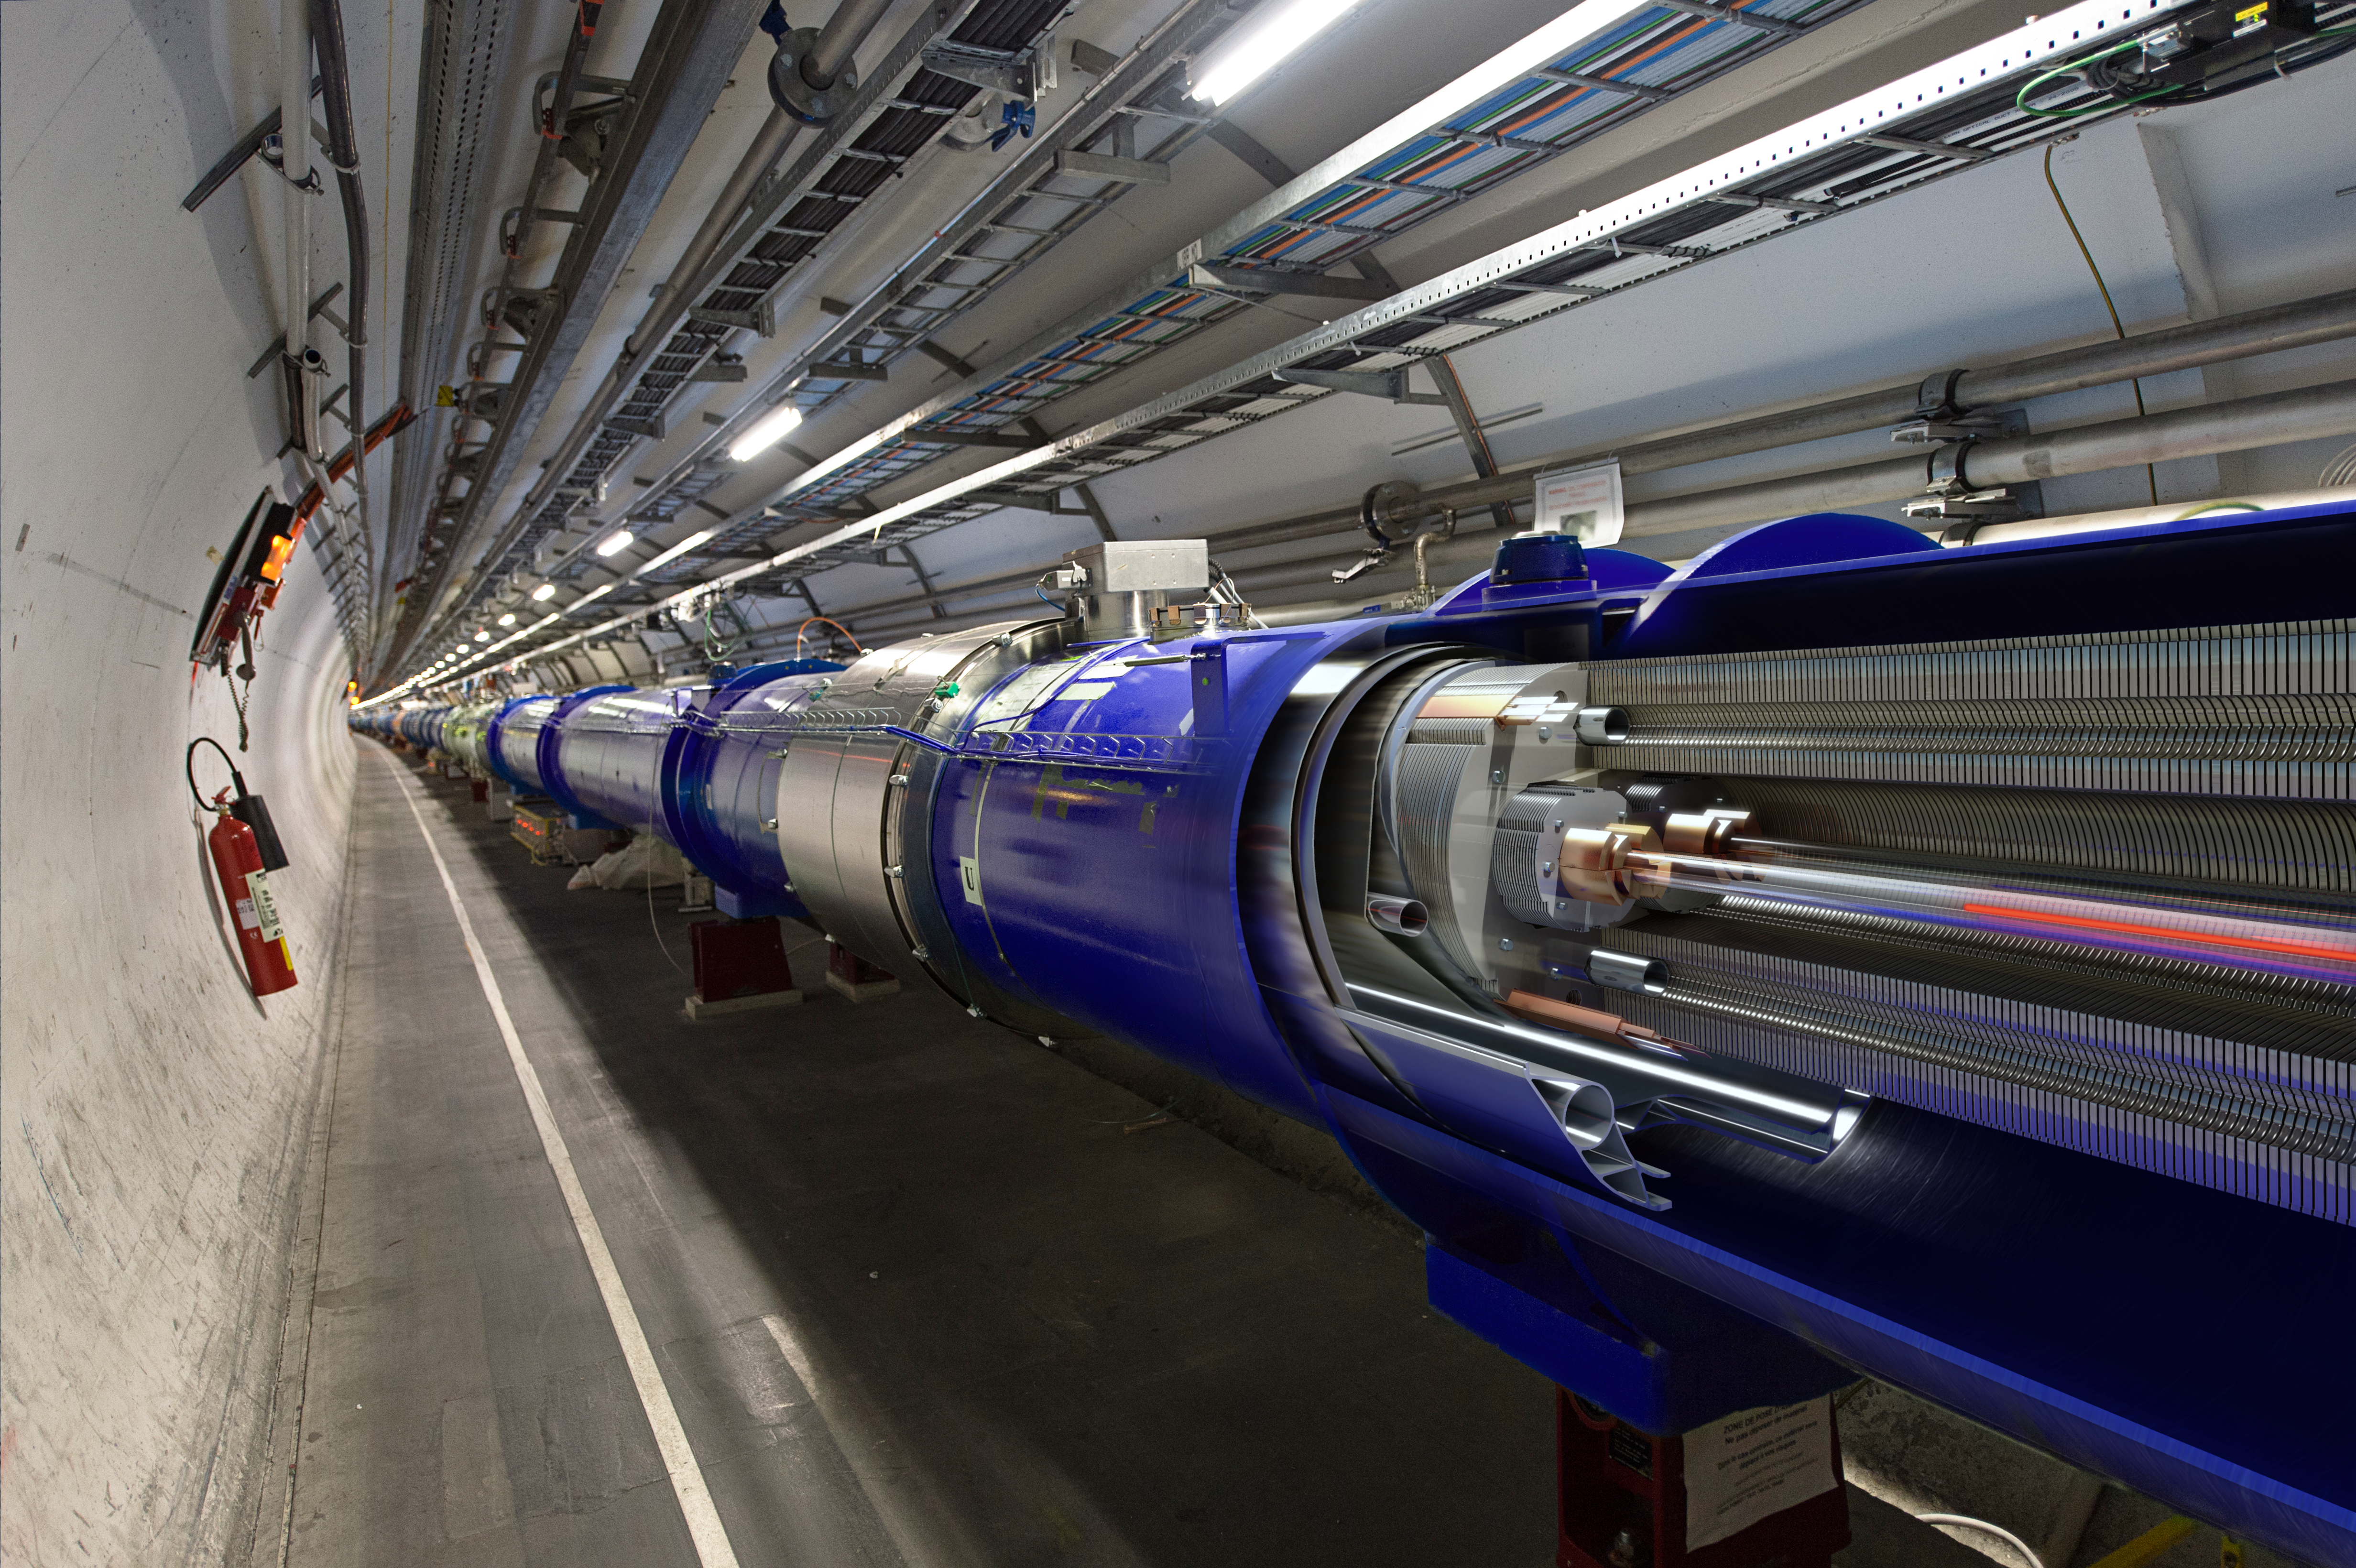
\includegraphics[width=0.8\textwidth]{chapters/01_Introduction/images/lhc_3D_cut.png}
    \caption{3D cut of a main LHC dipole~\cite{noauthor_cern_nodate}. Both beam pipes can be seen
    surrounded by the coils, strongly clamped by the yokes.}
    \label{fig:3d_cut_dipole}
\end{figure}


% -------------------------------
%   Straight Sections and Arcs
\subsubsection{\mread{Straight Sections and Arcs}}

The LHC is not a perfect circle. It is indeed composed of eight \textit{straight} sections, called
the \textit{Insertion Regions} (IRs) where detectors or specific instrumentation are placed.
Connecting those sections, the \textit{arcs} are where the majority of the magnets and their
correctors are located, along with some instrumentation like beam position monitors.
\Cref{fig:introduction:lhc_irs} shows the arcs as well as the purpose of each straight section.

\begin{figure}[!htb]
    \centering
    \includegraphics[width=0.5\textwidth]{./images/irs.png}
    \caption{Schematic of the LHC layout.}
    \label{fig:introduction:lhc_irs}
\end{figure}


% -------------------------------
%          Arc Cells
\subsubsection{\mread{Arc Cells}}

Each arc is made up of 23 cells. Magnets are organized in a standard FODO structure
(see \cref{section:courant_snyder}), as shown in \cref{fig:introduction:lhc_arc_cell}.
\textit{Dipoles} are responsible for bending the trajectory of the particles. Their associated
correctors, the orbit correctors, mitigate any possible drift in the path.
\textit{Quadrupoles} are used to control the beam size along the ring. Their effect is focusing in
one plane and defocusing in the other. Their associated correctors control the frequency of
oscillations of the beam (see tune, \cref{section:courant_snyder}) and possible field imperfections.
\textit{Sextupoles} correct chromaticity, a misfocus from quadrupoles due to particles having
a different momentum than the reference particle.
\textit{Octupoles} are used to stabilize the beam by introducing Landau
Damping~\cite{gareyte_landau_1997}. The associated correctors correct higher-order chromaticity
effects as well as amplitude-dependant tune shifts.
\textit{Decapoles} correctors aim at correcting an even higher chromaticity order.

\begin{figure}[H]
    \centering
    \includegraphics[width=1\textwidth]{./images/lhc_cell.png}
    \caption{Schematic of an LHC Arc cell~\cite{bruning_lhc_2004}.}
    \label{fig:introduction:lhc_arc_cell}
\end{figure}



% -------------------------------
%            Cycles
\subsubsection{\mread{Cycles}}

During the operation of the LHC, the machine goes through several states, each defined for specific 
scenarios~\cite{wenniger_lhc_2019}.

A common example is the operational cycle of the LHC, illustrated in \cref{fig:cern_complex:cycle}.
Initially, the magnets are pre-cycled~\cite{bottura_pre-cycles_2010} without any beam circulating,
to ensure a reproducible magnetic state. Their current is then increased to accept particles at the
injection energy of 450 GeV. To verify the machine's proper functioning, a probe bunch of reduced
intensity is first injected, at around $10^{10}$ particles. The number of bunches and their
intensity are then gradually increased to obtain the desired scheme needed for collisions, which
varies throughout the year based on experimental demands. The number of bunches and their intensity
can be adjusted as needed to ensure the machine's safety. A common scheme in 2024 is to inject about
2350 bunches, with around $1.5 \cdot 10^{11}$ particles in each bunch, for collisions. Optics
measurements, due to their destructive nature, typically use between one and three \textit{pilot}
bunches at a lower intensity of $10^{10}$ particles.

The current in the magnets is then increased along with adjustments in the phase and voltage of the
RF system to accelerate the particles to an energy of 6.8 TeV. During this ramp, the beam is
initially squeezed at the Interaction Points. However, further squeezing is limited by the
detectors' resolution, which is insufficient to accurately reconstruct a large number of collision
events simultaneously. Collisions then start, while levelling the $\beta^*$ at the ATLAS and CMS
experiments relative to the remaining beam intensity, ensuring optimal performance of the detectors.

\begin{figure}[!htb]
    \includegraphics[width=\textwidth]{./images/lhc_cycle.pdf}
    \caption{Simplified illustration of a standard LHC cycle. Adapted
    from~\cite{felix_soubelet_local_2023}.}
    \label{fig:cern_complex:cycle}
\end{figure}

% === Concepts of Accelerator Physics
\chapter{Concepts of Accelerator Physics}
\thumbforchapter{}
\chaptertoc{}
\newpage

\begin{enumerate}
    \tightlist
    \color{red}
    \item Hamiltonian
    \item Coordinates
    \begin{enumerate}
    \tightlist
        \item Courant Snyder, twiss parameters an phase space
        \item Linear Maps
        \item Non-Linear maps
        \item Normal Form \& RDT \& resonance diagram
    \end{enumerate}
    \item Linear optics: dispersion, coupling, momentum compaction
    \item Chromaticity

    \begin{enumerate}
    \tightlist
        \item Combined effect of multipoles
        \item Amplitude Detuning
        \item Chromtic Amplitude Detuning
        \item Dynamic Aperture
    \end{enumerate}
    \item Luminosity
\end{enumerate}



\input{chapters/02_Background/introduction.tex}
\section{Magnetic Fields}

% ============================================
%                Nomenclature
% ============================================
\subsection{\review{Nomenclature}}

Several notations coexist to denote magnetic fields. In this thesis, the
\textit{European Convention}~\cite{dilly_corrections_2022} is used for field indices, as shown
in Tab.~\ref{tab:magnetic_fields:relation_indices}. MAD-X, and MAD-NG, however, use the
\textit{American Convention}.

\begin{table}[H]
    \centering
    \begin{tabular}{l|c|c|c}
        Multipole     &      MAD-X        &     Index        & Normalized Strength \\
    \hline            
        Dipole        &     0             &     1            & $K_1$   \\       
        Quadrupole    &     1             &     2            & $K_2 $  \\
        Sextupole     &     2             &     3            & $K_3 $  \\
        Octupole      &     3             &     4            & $K_4 $  \\
        Decapole      &     4             &     5            & $K_5 $  \\
        Dodecapole    &     5             &     6            & $K_6 $  \\
        Decatetrapole &     6             &     7            & $K_7 $  \\
    \end{tabular}
    \caption{Relation between field indices and multipoles.}
    \label{tab:magnetic_fields:relation_indices}
\end{table}

As such, unless explicitly stated, quantities such as the magnetic strength $b$ and normalized
strength $K$ will be expressed with this notation. 


% ============================================
%              Multipole Expansion
% ============================================
\subsection{\review{Multipole Expansion}}

A 2 dimension magnetic field in the planes \textit{x} and \textit{y} can be described as a sum of
the normal and skew field gradients $\mathcal{B}$ and $\mathcal{A}$ with multipoles of order $n$,
given by~\cite{wolf_engineering_2001}:
\begin{equation}
    B_y + iB_x = \sum_{n=1}^\infty \left(\mathcal{B}_n + i\mathcal{A}_n \right)  (x+iy)^{n-1}
\end{equation}

An ideal magnet would produce either a sole normal or skew field. However, this is not applicable 
to real-life magnets that are imperfect, due to design and manufacturing constraints.
Field errors are thus introduced, relative to the main field of the ideal 2N-pole magnet at a
reference radius $r_{ref}$~\cite{dilly_corrections_2022}, as shown in 
Eq.~\eqref{eq:magnetic_field:relative_errors}. The coefficients of the normal and skew relative 
field errors, referred to as $a_n$ and $b_n$, are dimensionless but often given in \textit{units}
of $10^{-4}$.

\begin{equation}
    B_y + iB_x = 
        \begin{cases}
            \mathcal{B}_N \cdot \sum_{n+1}^\infty (b_n + ia_n) \left(\frac{x+iy}{r_{ref}}\right)^{n-1}\text{, for normal magnets}\\
            \mathcal{A}_N \cdot \sum_{n+1}^\infty (b_n + ia_n) \left(\frac{x+iy}{r_{ref}}\right)^{n-1}\text{, for skew magnets}
        \end{cases}
    \label{eq:magnetic_field:relative_errors}
\end{equation}


The normal and skew field components of order $n$ for an imperfect 2N-pole magnet is thus given by
the following equation:

\begin{equation}
    \begin{aligned}
        \mathcal{B}_n &= \mathcal{B}_N \cdot \frac{b_n}{r_{ref}^{n-1}}, \\
        \mathcal{A}_n &= \mathcal{A}_N \cdot \frac{a_n}{r_{ref}^{n-1}}.
    \end{aligned}
\end{equation}

The unit of the field is relative to the multipole order $n$: $[\text{Tm}^{1-n}]$.


% ============================================
%              Normalization
% ============================================
\subsection{\review{Beam Rigidity and Normalization}}

\subsubsection{\review{Beam Rigidity}}

The beam rigidity refers to the resistance of a particle moving through the accelerator to the
bending applied by the magnetic fields. It is derived from the Laurentz force~\cite{dilly_corrections_2022}
and relates the magnetic field $B$, the radius of curvature $\rho$ to the momentum $p$ and charge $q$
of the particle:

\begin{equation}
    B \rho = \frac{p}{q}
    \label{eq:magnetic_fields_beam_rigidity}
\end{equation}

It is of interest when designing an accelerator to set the maximum field as well as the required
radius of curvature for a specific momentum and particle.
An interesting metric of an accelerator is also its \textit{filling factor}, or percentage of
dipoles in the machine. It can be calculated via the radius of curvature: $f = \rho / r$. A low 
filling factors means more space for other magnets, collimators, beam instrumentation, etc.

\subsubsection{\review{Field Normalization}}

The Beam Rigidity is also used as a way to normalize magnetic field strengths in particle
accelerators where the momentum of the particle changes (i.e. acceleration).
Normalized Normal and Skew components $K_n$ and $J_n$ are given by~\cite{wolf_engineering_2001}:

\begin{equation}
    \begin{aligned}
        K_n =  \frac{q}{p} &(n-1)! \mathcal{B}_n, \\ 
        J_n =  \frac{q}{p} &(n-1)! \mathcal{A}_n.
    \end{aligned}
    \label{eq:magnetic_fields_normalized}
\end{equation}



% ============================================
%            Hamiltonian Dynamics
% ============================================
\subsection{Hamiltonian Dynamics}

\todo{link to lie algebra\\
poisson bracket is a link between hamiltonian and coordinate evolutions \\
Lie Algebra uses poisson brackets}

The Hamiltonian describing the motion for the transverse planes of a given multipole or order $n$ is
given by~\cite{keintzel_jacqueline_beam_nodate,tomas_direct_2003,franchi_studies_2006}:

\begin{equation}
    \begin{aligned}
        H &= \frac{q}{p} \Re \left[ \sum_{n>1} (\mathcal{B}_n + i\mathcal{A}_n) \frac{(x+iy)^n}{n} \right] \\
          &= \Re \left[ \sum_{n>1} (K_n + iJ_n) \frac{(x+iy)^n}{n!} \right].
    \end{aligned}
    \label{eq:hamiltonian_magnet}
\end{equation}

Quite often, when studying the effect of a magnet on the beam, only one component is required, and
the sum can thus be dropped.
The normal and skew fields can also be isolated in order to consider their effect only:

\begin{equation}
    \begin{aligned}
        N_n &= \frac{1}{n!} K_n \Re \left[ (x+iy)^n \right] \\
        S_n &= -\frac{1}{n!} J_n \Im \left[ (x+iy)^n \right].
    \end{aligned}
    \label{eq:normal_skew_hamiltonian_magnet}
\end{equation}




\section{Coordinate Systems}

In circular accelerators, particle dynamics are represented using a traveling coordinate system.
A reference orbit is determined by the lattice and its magnet strengths, forming the
\textit{optics}. In the case of a synchrotron, like the LHC, where the particles return to their
original location after some turns, the reference orbit is also called the closed orbit.  
The Frenet-Serret coordinate system is used, moving along the ring on the reference orbit. The
coordinates are then transverse: $x$ and $y$, and longitudinal in the direction of travel: $s$.
Figure~\ref{fig:coordinate_systems:frenet_serret} shows those coordinates.

\begin{figure}[H]
    \centering
    \includegraphics[width=0.6\textwidth]{example-image-a}
    \caption{\todo{Frenet-Serret coordinates commonly used in accelerator physics.}}
    \label{fig:coordinate_systems:frenet_serret}
\end{figure}



% ============================================
%               Linear Lattice 
% ============================================
\subsection{Linear Lattice}

A circular accelerator is composed of many multipoles of different orders. A basic
design only requires dipoles and quadrupoles in order to operate. Dipoles are used to bend the
particles in order to form the ring, whereas quadrupoles are used to focus the beam to a focal
point, similar to light optics.
Those elements can be arranged in a particular order, to form a \text{FODO} cell. Such cells present
an alternating placement of focusing an defocusing quadrupoles with dipoles in between, as shown in
Fig.\ref{fig:coordinate_systems:fodo}, and are usually repeated many times along the ring.

\begin{figure}[H]
    \centering
    \includegraphics[width=0.6\textwidth]{example-image-a}
    \caption{\todo{FODO cell, a repeated basic block present in most circular accelerators.}}
    \label{fig:coordinate_systems:fodo}
\end{figure}

A lattice composed on of only dipoles and quadrupoles, is referred to as a \textit{linear} lattice.

\todo{
    Courant Snyder/Twiss
    Tune, beta function
% 
    Lie, normal form
    Resonance Driving Terms
}
\section{Resonances}


%----------------------------------------
%
%----------------------------------------

\begin{figure}[H]
    \centering
    \includegraphics[width=0.7\textwidth]{images/resonance_diagaram_n5.png}
    \caption{Tune diagram with resonances lines excited by multipoles up to decapole ($n \leq 5$).
             The working point of the machine is chosen in an area where few lines are present.}
    \label{fig:resonances:diagram_n5}
\end{figure}


\begin{figure}[H]
    \centering
    \includegraphics[width=0.7\textwidth]{images/resonance_diagaram_n7.png}
    \caption{Tune diagram with resonances lines excited by multipoles up to decatetrapole 
             ($n \leq 7$). When considering higher orders, it becomes apparent that the beam will
             hit several resonances.}
    \label{fig:resonances:diagram_n7}
\end{figure}
\section{Detuning Effects}


% ============================================
%                Chromaticity
% ============================================
\subsection{\review{Chromaticity}}

Chromaticity is the tune change $\Delta Q$ relative to the momentum offset $\delta$. Chromaticity
can be described by a Taylor expansion, given by

\begin{equation} 
    Q (\delta) = Q_0 + Q' \delta + \frac{1}{2!} Q'' \delta^2 + \frac{1}{3!} Q''' \delta^3 + \mathcal{O}(\delta^4).
    \label{eq:background_chromaticity}
\end{equation}

Or, more generally, rewritten as a sum to include all orders up to $n$:

\begin{equation}
    Q (\delta) = Q_0 + \sum_{i=1}^n \frac{1}{i!} Q^{(i)} \delta^i.
    \label{eq:background_chromaticity_sum}
\end{equation}


The first order of the chromaticity expansion, $Q'$, is generally simply referred to as 
\textit{chromaticity}, sometimes as \textit{linear chromaticity}.
The other terms are thus referred to as \textit{non-linear chromaticity}.

The chromaticity change induced by a single element of order $n$ and length $L$ can be derived from
the Hamiltonian of Eq.~\eqref{eq:hamiltonian_magnet}, averaging over the phase variables and
differentiating relative to the actions $J_{x,y}$ and the momentum offset $\delta$:

\begin{equation}
    \Delta Q^{(n)}_{x,y} = \frac{\partial^n Q_{x,y}}{\partial^n \delta} = 
      \frac{1}{2\pi} \int_L \left< \frac{\partial^{(n+1)} H}{\partial J_{x,y}\partial^n \delta}\right> \diff s.
    \label{eq:background_chroma_order_hamiltonian}
\end{equation}


% =========
\subsubsection{Natural Chromaticity from Quadrupoles}

In a purely linear lattice, the linear chromaticity, $Q'$, is a result of the momentum dependence 
of the quadrupoles' focusing. It is in this case called the \textit{natural chromaticity} and can be
derived from the normal hamiltonian of Eq.\eqref{eq:normal_skew_hamiltonian_magnet} and expressing
the normalized magnet strength $K$ with a dependence on $\delta$ via $P$ as $P_0(1+\delta)$:

\begin{equation}
    K_n = \frac{q}{P_0} \frac{1}{1 + \delta} (n - 1)! B_n
    \label{eq:k_dpp}
\end{equation}

The normal field of a quadrupole is then given by

\begin{equation}
    \mathcal{N}_2(x,y) = \frac{1}{2} \frac{q}{P_0} \frac{1}{1+\delta} B_2 (x^2 - y^2)
\end{equation}

By operating a variable change to the angle coordinates 
(\(x \rightarrow \sqrt{2 J_x \beta_x} \cos \phi_x\) and
\(y \rightarrow \sqrt{2 J_y \beta_y} \cos \phi_y\)), the following equation linking the $\beta$-function
and $\delta$ to the normal field is obtained:
\begin{equation}\mathcal{N}_2 (x,y) = \frac{1}{2} \frac{q}{P_0} \frac{1}{1+\delta} B_2 
        \left[
            \left(\sqrt{2 J_x \beta_x} \cos \phi_x \right)^2 
            - \left(\sqrt{2 J_y \beta_y} \cos \phi_y\right)^2
        \right].
    \label{eq:hamiltonian_quadrupole_angle}
\end{equation}

Following Eq.\eqref{eq:background_chroma_order_hamiltonian}, the natural chromaticity $Q'$ induced by
quadrupoles is given by:
\begin{equation}
    \begin{aligned}
        \Delta Q'_x &= \frac{1}{2\pi} \int_L \frac{\partial^2 \left< \mathcal{N}_2 \right> }{\partial J_x \partial \delta} \diff s
        \quad;\quad
        \Delta Q'_y &= \frac{1}{2\pi} \int_L \frac{\partial^2 \left< \mathcal{N}_2 \right>}{\partial J_y \partial \delta} \diff s
        \\
        & = - \frac{1}{4 \pi} \frac{q}{P_0} B_2 L \beta_x
        & = \frac{1}{4 \pi} \frac{q}{P_0} B_2 L \beta_y
    \end{aligned}
\end{equation}


% =========
\subsubsection{Linear Chromaticity from Sextupoles}

The first order chromaticity $Q'$ is contributed to by sextupoles in the presence of off-momentum
particles. The normal field of a sextupole, following Eq.\eqref{eq:normal_skew_hamiltonian_magnet}
is given by

\begin{equation}
    \mathcal{N}_3(x,y) = \frac{1}{3!} (x^3 - 3xy^2).
    \label{eq:detuning:linear_chromaticity}
\end{equation}

As the momentum offset $\delta$ introduces a change in orbit via
dispersion~\cite{keintzel_second-order_2019}, a variable change can be operated on both $x$ and $y$,
as shown in Eq.\eqref{eq:detuning:offset}. In this thesis, vertical dispersion will be though
neglected.

\begin{equation}
    \begin{aligned}
        x &\rightarrow x + \Delta x = x + D_x\delta \\
        y &\rightarrow y + \Delta y = y + D_y\delta
    \end{aligned}
    \label{eq:detuning:offset}
\end{equation}

The positions $x$ and $y$ can once be replaced, using the twiss parameters, giving the full
expression:

\begin{equation}\begin{aligned}
  \mathcal{N}_3(x + \Delta x, y) = \frac{1}{6} K_3 \biggl[&
       \left(\sqrt{2 J_x \beta_x} \cos \phi_x\right)^3 \\
  &    + 3 \left(\sqrt{2 J_x \beta_x} \cos \phi_x\right)^2 D_x \delta \\
  &    + 3 \left(\sqrt{2 J_x \beta_x} \cos \phi_x\right) D_x^2 \delta^2 \\
  &    + D_x^3 \delta^3 \\
  &    - 3 \left(\sqrt{2 J_x \beta_x} \cos \phi_x \right) \left(\sqrt{2 J_y \beta_y} \cos \phi_y \right)^2 \\
  &    - 3 D_x \delta (\sqrt{2 J_y \beta_y} \cos \phi_y)^2 \biggl]
\end{aligned}\end{equation}

Averaging over the phase variables removes any odd cosine:
\begin{equation}\begin{aligned}
  \left< \mathcal{N}_3(x + \Delta x, y) \right> = \frac{1}{6} K_3 &\biggl(
       3 J_x \beta_x D_x \delta \\
  &    + D_x^3 \delta^3 \\
  &    - 3 D_x \delta J_y \beta_y \biggl)
\end{aligned}\end{equation}



The chromaticity can then obtained by differentiating relative to the action $J_{x,y}$ to obtain the
tune, and then by the momentum offset $\delta$.
\begin{equation}
    \begin{aligned}
        \Delta Q'_x &= \frac{1}{2\pi} \int_L \frac{\partial^2 \left< \mathcal{N}_3 \right>}{\partial J_x \partial \delta} \diff s \quad; \quad \Delta Q'_y &&= \frac{1}{2\pi} \int_L \frac{\partial^2 \left< \mathcal{N}_3 \right>}{\partial J_y \partial \delta} \diff s \\
        &= \frac{1}{2 \pi} L \frac{1}{2} K_3 \beta_x D_x  &&= - \frac{1}{2 \pi} L \frac{1}{2} K_3 \beta_y D_x \\
        &= \frac{1}{4 \pi}  K_3 L \beta_x D_x &&= - \frac{1}{4 \pi}  K_3 L \beta_y D_x
    \end{aligned}
\end{equation}

From this last equation, it is apparent than sextupoles are not a source of chromaticity of higher
orders in the presence of linear dispersion. In the presence of second order
dispersion~\cite{keintzel_second-order_2019}, sextupoles can generate some amount of $Q''$, usually
negligible.


% =========
\subsubsection{Non-Linear Chromaticity}

Higher orders of the chromaticity function are described in~\cite{dilly_derivation_2023} and follow
the same logic as for the linear chromaticity from sextupoles.





% ============================================
%             Amplitude Detuning
% ============================================
\subsection{Amplitude Detuning}



% ============================================
%        Chromatic Amplitude Detuning
% ============================================
\subsection{Chromatic Amplitude Detuning}

\todo{make it clear I derived it}
\chapter{Optics Measurements and Corrections}

% === Beam Instrumentation
\section{Beam Instrumentation}

% === Measurements
\section{Optics Measurements}

% tbt
% chromaticity

\section{Correction Concepts}
\chapter{\review{Skew Octupolar Fields}}
\label{chapter:skew_octupole_fields}
\thumbforchapter{}


%=============================
%        Introduction
%=============================
\section{\review{Introduction}}

The skew octupolar fields in the LHC have previously been identified as significant contributors to 
limits in forced dynamic aperture, being the dynamic aperture when kicking the beam with the
AC-Dipole~\cite{carlier_nonlinear_2020}. Skew octupolar correctors are positioned around the
ATLAS and CMS detectors, in Interaction Regions 1 and 5. Those correctors are \textit{common
aperture} magnets ; both beams are affected by the created magnetic fields. Unfortunately, one of
these four correctors, located to the left of ATLAS, is not functioning. As a result, although
corrections can be calculated, they will not effectively minimize the skew octupolar RDTs of
interest, $f_{1012,y}$ and $f_{1210,x}$. 
The associated resonances and frequency lines of these RDTs are shown in
\cref{tab:skew_octupolar:resonances_rdts}.

\begin{table}[!htb]
    \centering
    \begin{tabular}{lccc}
      \toprule
      RDT         & Resonance                &  H-line                    & V-line         \\
      \midrule
      $f_{1012}$  & $\phantom{-}1Q_x - 1Q_y$ &  $\phantom{2Q_x-\ \,}1Q_y$ & $-1Q_x + 2Q_y$ \\
      $f_{1210}$  & $-1Q_x + 1Q_y$           &  $2Q_x - 1Q_y$             & $\phantom{-}1Q_x\phantom{+2Q_y\ \,}$    \\
      \bottomrule
    \end{tabular}
    \caption{Skew octupolar RDTs of interest, their associated resonances and the frequency spectrum
    lines they contribute to.}
    \label{tab:skew_octupolar:resonances_rdts}
\end{table}

First corrections of skew octupolar RDTs were performed in 2018 at top
energy~\cite{carlier_nonlinear_2020}. A different approach for the same corrections is presented in
this chapter.
Measurements were also performed at injection energy with the prospect of corrections. However, it
was observed that Landau octupoles were strongly contributing to the RDTs of interest.


%=============================
%         Top Energy
%=============================
\section{\review{Corrections at Top Energy}}

The very first skew octupolar RDT corrections in the LHC were made in 2018 during
Run~2~\cite{carlier_nonlinear_2020}. These corrections were computed by matching the RDT level of
the measurements in simulation and then inverting the strengths. This is possible and remains viable
as only three correctors are used and values can be manually adjusted.
In this section, a different approach is taken, based on response matrices. This type of correction
is explained in details in \cref{correction_principle:response_matrix}. The real and imaginary 
responses of the RDTs for each corrector at an arbitrary strength are simulated through tracking.
These responses are collected into a matrix, allowing the determination of the required strengths to
match the RDT level observed in the measurements. Inverting these values result in a correction.


%-----------------------------
%     Correctors Response
%-----------------------------
\subsection{\review{Correctors}}

To create a response matrix, simulations were conducted with the tunes and AC-Dipole deltas set to
those used for measurements. The natural tunes are $Q_x = 0.285$ and $Q_y = 0.292$ while the driven
tunes are $\Delta Q_x = -0.008$ and $\Delta Q_y = 0.01$. Each corrector is then powered
individually for each tracking simulation. For this type of simulation, field errors are not
necessary, as only the RDT shift caused by the corrector relative to the baseline is needed.
\Cref{fig:skew_octupolar:response_correctors} shows the real part of the resulting RDTs from these
simulations for Beam 1. Beam 2 shows a similar level of response for these correctors.

\begin{figure}[!htb]
    \centering
    \begin{subfigure}{0.8\textwidth}
        \includegraphics[width=\textwidth]{./images/f1012_b1_correctors.pdf}
        \caption{$f_{1012,y}$}
    \end{subfigure}
    \par\bigskip 
    \begin{subfigure}{0.8\textwidth}
        \includegraphics[width=\textwidth]{./images/f1210_b1_correctors.pdf}
        \caption{$f_{1210,x}$}
    \end{subfigure}
    \caption{Simulation of the RDT response of the skew octupolar correctors at top energy for Beam
    1. Each corrector is powered at $J_4 = 1 [\text{m}^{-4}]$.}
    \label{fig:skew_octupolar:response_correctors}
\end{figure}

It can already be seen that the L5 and R5 correctors show a similar trend along the ring, with L5
showing a stronger response for the same strength, while the R1 corrector follows the opposite
trend. A polar plot at a given BPM can illustrate that trend, and be used to get an intuition of the
effect of the correctors to manually compute corrections.
\Cref{fig:skew_octupolar:response_correctors_polar} shows the orthogonality of the correctors for
both beams and RDTs. L5 being stronger than R5 while having the same angle indicates that only one
of them is needed for corrections. 

\begin{figure}[!htb]
    \centering
    \begin{subfigure}{0.8\textwidth}
        \includegraphics[width=\textwidth]{./images/orthogonal_a4_inj_f1012_y.pdf}
        \caption{$f_{1012,y}$}
    \end{subfigure}
    \par\bigskip 
    \begin{subfigure}{0.8\textwidth}
        \includegraphics[width=\textwidth]{./images/orthogonal_a4_inj_f1210_x.pdf}
        \caption{$f_{1210,x}$}
    \end{subfigure}
    \caption{Simulated RDTs response of the available skew octupolar correctors at top energy.  Each
    corrector is powered at $J_4 = 1 [\text{m}^{-4}]$. The orthogonality of R1 and L5/R5 allows to
    independently control the real and imaginary parts.}
    \label{fig:skew_octupolar:response_correctors_polar}
\end{figure}



%-----------------------------
%         Correction
%-----------------------------
\subsection{\review{Measurements and Corrections}}

Initial measurements of the machine at top energy ($\beta^*=30$cm) without any skew octupolar
correctors were done during an MD slot in 2022 to determine the level of the RDTs before being able
to correct them. Those measurements were made at natural tunes of $Q_x = 0.285$ and $Q_y = 0.292$.
The driven tunes were set to $\Delta Q_x = -0.008$ and $\Delta Q_y = 0.01$. This selection of tunes
has proven to be appropriate for measuring skew octupolar RDTs. The Landau octupoles were powered
off during the measurements. 

The corrections were computed via the previously detailed response matrix and are shown in
\cref{tab:skew_octupolar:correction_strengths}. These have then been applied during 2023's
commissioning and later on kept for operation. The RDT levels of the bare machine and with these
corrections are shown in \cref{fig:skew_octupolar:corrections_vs_bare}. It can be observed that both
RDT amplitudes are reduced, with the exception of $f_{1210,x}$ for Beam 2, which stays constant.
The reduction of RDT amplitude is comparable to those obtained in 2018, where the same RDT for Beam
2 did neither improve or worsen.


\begin{table}[!htb]
    \centering
    \begin{tabular}{lr}
      \toprule
      Corrector    &    Strength $[\text{m}^{-4}]$ \\
      \midrule
      MCOSX3.L1    &                —  \\
      MCOSX3.R1    &           $-0.50$ \\
      MCOSX3.L5    &           $ 0.42$ \\
      MCOSX3.R5    &           $-0.01$ \\
      \bottomrule
    \end{tabular}
    \caption{Computed corrections for skew octupolar RDTs at top energy. The corrector L1 has been 
    broken for several years and can not be used.}
    \label{tab:skew_octupolar:correction_strengths}
\end{table}
 
\begin{figure}[!htb]
    \centering
    \begin{subfigure}{0.49\textwidth}
        \includegraphics[width=\textwidth]{./images/f1012_b1.pdf}
        \caption{$f_{1012,y}$ Beam 1}
    \end{subfigure}
    \hfill
    \begin{subfigure}{0.49\textwidth}
        \includegraphics[width=\textwidth]{./images/f1012_b2.pdf}
        \caption{$f_{1012,y}$ Beam 2}
    \end{subfigure}
    %
    \par\bigskip 
    % 
    \begin{subfigure}{0.49\textwidth}
        \includegraphics[width=\textwidth]{./images/f1210_b1.pdf}
        \caption{$f_{1210,x}$ Beam 1}
    \end{subfigure}
    \hfill
    \begin{subfigure}{0.49\textwidth}
        \includegraphics[width=\textwidth]{./images/f1210_b2.pdf}
        \caption{$f_{1210,x}$ Beam 2}
    \end{subfigure}
    \caption{Measured skew octupolar RDTs at top energy and $\beta^*=30\text{cm}$ before and after
    correction. A reduction if observed for all but one RDT in Beam 2.} 
    \label{fig:skew_octupolar:corrections_vs_bare}
\end{figure}






%=============================
%    Landau Contribution
%=============================
% https://indico.cern.ch/event/1351567/contributions/5708754/attachments/2773145/4832599/2023-12-15_MO_Roll_Coupling_complete.pdf
\FloatBarrier
\section{\review{Landau Octupoles Contribution}}


%-----------------------------
%        Introduction
%-----------------------------
\subsection{\review{Introduction}}

During the 2023 commissioning, measurements were taken at injection energy with different strengths
of Landau octupoles, where an unexpected shift in the skew octupolar RDTs was observed. Subsequent
measurements were conducted to better understand and characterize this contribution of normal
octupoles to skew octupolar fields. These new measurements were taken during an MD slot in September
2023 and focused on varying the strengths of the Landau octupoles to $-1K_4$, $\pm2 K_4$, $5K_4$.
All measurements were taken at injection energy at tunes of $Q_x = 0.275$, $Q_y = 0.293$ and
AC-Dipole deltas of $\Delta Q_x = -0.01$ and $\Delta Q_y = -0.011$. Although both beams were
measured, this section focuses on Beam 1 to preliminarily investigate the matter.  The following
\cref{fig:skew_octupolar:mo_different_levels_meas} illustrates the difference in amplitude of the
RDT $f_{1012}$ with these varying strengths.
\Cref{fig:skew_octupolar:mo_meas_vs_sim_+2} on the other hand shows the measured and simulated shift
of the same RDT from $0K_4$ to $+2K_4$. It is evident that simulations including normal and skew 
octupolar field errors are not enough to explain the behaviour observed in the measurements.

\begin{figure}[!htb]
    \centering
    \begin{subfigure}{0.8\textwidth}
        \includegraphics[width=\textwidth]{./images/skew_octupoles/f1210_AMP_all_measurements.pdf}
    \end{subfigure}
    \caption{Unexpected difference of skew octupolar RDT amplitudes with varying Landau octupoles
    strengths.}
    \label{fig:skew_octupolar:mo_different_levels_meas}
\end{figure}

\begin{figure}[!htb]
    \centering
    \begin{subfigure}{0.8\textwidth}
        \includegraphics[width=\textwidth]{./images/skew_octupoles/f1012_meas_vs_sim_0shift.pdf}
        %\caption{$f_{1012,y}$}
    \end{subfigure}
    \caption{Measured and simulated shift of skew octupolar RDT after increase of Landau octupoles
    strength from zero. It is apparent that the shift in measurement is not replicated by the
    simulation.}
    \label{fig:skew_octupolar:mo_meas_vs_sim_+2}
\end{figure}



%-----------------------------
%        Misalignments
%-----------------------------
\subsection{\review{Misalignments}}

Magnet misalignments, more specifically roll errors, can generate skew magnetic fields instead of
the expected normal ones. To determine if this could explain the behaviour observed in measurements,
a tracking simulation was conducted with and without roll errors applied to the Landau octupoles.
The resulting RDTs reveal an imperceptible difference, unable to account for  the previously seen
shifts. The real part of the RDT $f_{1012}$ is shown in \cref{fig:skew_octupolar:sim_misalign},
with similar results seen in the other component and in $f_{1210}$.

\begin{figure}[!htb]
    \centering
    \begin{subfigure}{0.8\textwidth}
        \includegraphics[width=\textwidth]{./images/skew_octupoles/f1012_misalign_REAL.pdf}
        %\caption{$f_{1012,y}$}
    \end{subfigure}
    \caption{Simulated skew octupolar RDT with normal and skew octupolar errors and Landau octupoles
    powered. One simulation includes further alignment errors on the Landau octupoles. No 
    significant difference is observed between the two.}
    \label{fig:skew_octupolar:sim_misalign}
\end{figure}



%-----------------------------
%        Coupling
%-----------------------------
\subsection{\review{Coupling}}

As misalignments could not explain the discrepancy, simulations were first run with varying values
of coupling at a fixed octupolar strength, allowing to gage the impact of coupling only.
\Cref{appendix:transfer_map:skew_quadrupole_and_octupole} details how coupling, in the form of a
skew quadrupole, combined with a normal octupole can generate skew quadrupolar-like fields.
The resulting RDT $f_{1012}$ is shown in \cref{fig:skew_octupolar:sim_coupling}, a similar trend is
observed for $f_{1210}$.
The presented $C^{-}$ values are commonly seen in operation and well below that of the
tolerances of the design of the LHC~\cite{bruning_lhc_2004}. As coupling increases, the skew
octupolar RDTs are expected to be significantly altered.

\begin{figure}[!htb]
    \centering
    \begin{subfigure}{0.8\textwidth}
        \includegraphics[width=\textwidth]{./images/skew_octupoles/f1012_coupling_sim_AMP.pdf}
    \end{subfigure}
    \caption{Simulated skew octupolar RDT with fixed Landau octupole strength but varying coupling.
    Selected coupling values are often seen in operation.}
    \label{fig:skew_octupolar:sim_coupling}
\end{figure}



%-----------------------------
%          Responses
\FloatBarrier
\subsubsection{\review{Responses with Coupling}}

\begin{table}[!htb]
    \centering
    \begin{tabular}{cccc}
    \toprule
    &&\multicolumn{2}{c}{Rel. Diff. [\%]} \\
    \cmidrule{3-4}
    $K_4$ $[\text{m}^{-4}]$ & RDT & Real & Imag. \\
    \midrule
    \multirow{2}{*}{+5}
     & $f_{1210}$ & 6 & 6  \\
     & $f_{1012}$ & 12  & 11 \\[0.5em]
    \multirow{2}{*}{+2}
     & $f_{1210}$ & 32  & 34  \\
     & $f_{1012}$ & 36  & 36  \\[0.5em]
    \multirow{2}{*}{-1}
     & $f_{1210}$ & 26 & 25 \\
     & $f_{1012}$ & 21 & 20 \\[0.5em]
    \multirow{2}{*}{-2}
     & $f_{1210}$ & 19  & 17  \\
     & $f_{1012}$ & 21 & 20 \\
    \bottomrule
    \end{tabular}
    \caption{Relative difference between measured and simulated RDT shift induced by the
    Landau octupoles in presence of coupling. Real parts are illustrated in
    \cref{fig:skew_octupolar:response_meas_sim_coupling}.}
    \label{tab:skew_octupolar:rms_ratios}
\end{table}

After having demonstrated that coupling could significantly contribute to the creation of skew
octupolar fields with normal octupoles, additional simulations were performed matching the measured
coupling for each set of measurements. The shift in real part of the RDTs $f_{1012}$ and $f_{1210}$
is shown in \cref{fig:skew_octupolar:response_meas_sim_coupling}, with a similar pattern observed
for the imaginary part. The relative RMS deviation between simulations and measurements is given
for each set of strengths and RDTs in \cref{tab:skew_octupolar:rms_ratios}.

It can be observed that simulations and measurements for positive strengths ($K_4=2$ and $K_4=5$) 
are now in good agreement. This suggests that the primary contribution to the skew octupolar RDTs
can be attributed to the Landau octupoles and coupling. The relative deviation between measurement
and simulation can be explained by the sensitivity to the coupling. A difference of $10^{-4}$ units 
is enough to be noticeable, making accurate reproduction of skew octupolar RDTs not trivial.
It is important to note that measurements of $f_{1012}$ with \textit{negative} strength show a
response opposite to what is predicted by simulations while $f_{1210}$ agrees well. This behaviour
is not yet understood and requires further investigation.

\begin{figure}[!htb]
    \centering
    \begin{subfigure}{0.47\textwidth}
        \includegraphics[width=\textwidth]{./images/skew_octupoles/responses_coupling/f1012_response_meas_sim_+5_REAL_smoll.pdf}
        %\caption{$f_{1012,y}$ for $K_4 = +5$}
    \end{subfigure}
    \hfill
    \begin{subfigure}{0.47\textwidth}
        \includegraphics[width=\textwidth]{./images/skew_octupoles/responses_coupling/f1210_response_meas_sim_+5_REAL_smoll.pdf}
        %\caption{$f_{1210,x}$ for $K_4 = +5$}
    \end{subfigure}
    %
    \par\medskip 
    %
    \begin{subfigure}{0.47\textwidth}
        \includegraphics[width=\textwidth]{./images/skew_octupoles/responses_coupling/f1012_response_meas_sim_+2_REAL_smoll.pdf}
        %\caption{$f_{1012,y}$ for $K_4 = +2$}
    \end{subfigure}
    \hfill
    \begin{subfigure}{0.47\textwidth}
        \includegraphics[width=\textwidth]{./images/skew_octupoles/responses_coupling/f1210_response_meas_sim_+2_REAL_smoll.pdf}
        %\caption{$f_{1210,x}$ for $K_4 = +2$}
    \end{subfigure}
    %
    \par\medskip 
    %
    \begin{subfigure}{0.47\textwidth}
        \includegraphics[width=\textwidth]{./images/skew_octupoles/responses_coupling/f1012_response_meas_sim_-1_REAL_smoll.pdf}
        %\caption{$f_{1012,y}$ for $K_4 = -1$}
    \end{subfigure}
    \hfill
    \begin{subfigure}{0.47\textwidth}
        \includegraphics[width=\textwidth]{./images/skew_octupoles/responses_coupling/f1210_response_meas_sim_-1_REAL_smoll.pdf}
        %\caption{$f_{1210,x}$ for $K_4 = -1$}
    \end{subfigure}
    %
    \par\medskip
    %
    \begin{subfigure}{0.47\textwidth}
        \includegraphics[width=\textwidth]{./images/skew_octupoles/responses_coupling/f1012_response_meas_sim_-2_REAL_smoll.pdf}
        %\caption{$f_{1012,y}$ for $K_4 = -2$}
    \end{subfigure}
    \hfill
    \begin{subfigure}{0.47\textwidth}
        \includegraphics[width=\textwidth]{./images/skew_octupoles/responses_coupling/f1210_response_meas_sim_-2_REAL_smoll.pdf}
        %\caption{$f_{1210,x}$ for $K_4 = -2$}
    \end{subfigure}
    \caption{Measured and simulated real part shift of skew octupolar RDTs induced by Landau
    octupoles in presence of coupling at injection energy. Left column shows $f_{1012}$ while right
    shows $f_{1210}$.}
    \label{fig:skew_octupolar:response_meas_sim_coupling}
\end{figure}


% Imaginary Parts
%\begin{figure}[!htb]
%    \centering
%    \begin{subfigure}{0.47\textwidth}
%        \includegraphics[width=\textwidth]{./images/skew_octupoles/responses_coupling/f1012_response_meas_sim_+5_IMAG_smoll.pdf}
%        %\caption{$f_{1012,y}$ for $K_4 = +5$}
%    \end{subfigure}
%    \hfill
%    \begin{subfigure}{0.47\textwidth}
%        \includegraphics[width=\textwidth]{./images/skew_octupoles/responses_coupling/f1210_response_meas_sim_+5_IMAG_smoll.pdf}
%        %\caption{$f_{1210,x}$ for $K_4 = +5$}
%    \end{subfigure}
%    %
%    \par\medskip 
%    %
%    \begin{subfigure}{0.47\textwidth}
%        \includegraphics[width=\textwidth]{./images/skew_octupoles/responses_coupling/f1012_response_meas_sim_+2_IMAG_smoll.pdf}
%        %\caption{$f_{1012,y}$ for $K_4 = +2$}
%    \end{subfigure}
%    \hfill
%    \begin{subfigure}{0.47\textwidth}
%        \includegraphics[width=\textwidth]{./images/skew_octupoles/responses_coupling/f1210_response_meas_sim_+2_IMAG_smoll.pdf}
%        %\caption{$f_{1210,x}$ for $K_4 = +2$}
%    \end{subfigure}
%    %
%    \par\medskip 
%    %
%    \begin{subfigure}{0.47\textwidth}
%        \includegraphics[width=\textwidth]{./images/skew_octupoles/responses_coupling/f1012_response_meas_sim_-1_IMAG_smoll.pdf}
%        %\caption{$f_{1012,y}$ for $K_4 = -1$}
%    \end{subfigure}
%    \hfill
%    \begin{subfigure}{0.47\textwidth}
%        \includegraphics[width=\textwidth]{./images/skew_octupoles/responses_coupling/f1210_response_meas_sim_-1_IMAG_smoll.pdf}
%        %\caption{$f_{1210,x}$ for $K_4 = -1$}
%    \end{subfigure}
%    %
%    \par\medskip
%    %
%    \begin{subfigure}{0.47\textwidth}
%        \includegraphics[width=\textwidth]{./images/skew_octupoles/responses_coupling/f1012_response_meas_sim_-2_IMAG_smoll.pdf}
%        %\caption{$f_{1012,y}$ for $K_4 = -2$}
%    \end{subfigure}
%    \hfill
%    \begin{subfigure}{0.47\textwidth}
%        \includegraphics[width=\textwidth]{./images/skew_octupoles/responses_coupling/f1210_response_meas_sim_-2_IMAG_smoll.pdf}
%        %\caption{$f_{1210,x}$ for $K_4 = -2$}
%    \end{subfigure}
%    \caption{Measured and simulated imaginary part shift of skew octupolar RDTs induced by Landau
%    octupoles in presence of coupling at injection energy. Left column shows $f_{1012}$ while right
%    shows $f_{1210}$.}
%    \label{fig:skew_octupolar:response_meas_sim_coupling_imag}
%\end{figure}


% Constant coupling
%\begin{figure}[!htb]
%    \centering
%    \begin{subfigure}{0.47\textwidth}
%        \includegraphics[width=\textwidth]{./images/skew_octupoles/responses_coupling/f1012_response_meas_sim_+5_REAL_smoll_const_coupling.pdf}
%        %\caption{$f_{1012,y}$ for $K_4 = +5$}
%    \end{subfigure}
%    \hfill
%    \begin{subfigure}{0.47\textwidth}
%        \includegraphics[width=\textwidth]{./images/skew_octupoles/responses_coupling/f1210_response_meas_sim_+5_REAL_smoll_const_coupling.pdf}
%        %\caption{$f_{1210,x}$ for $K_4 = +5$}
%    \end{subfigure}
%    %
%    \par\medskip 
%    %
%    \begin{subfigure}{0.47\textwidth}
%        \includegraphics[width=\textwidth]{./images/skew_octupoles/responses_coupling/f1012_response_meas_sim_+2_REAL_smoll_const_coupling.pdf}
%        %\caption{$f_{1012,y}$ for $K_4 = +2$}
%    \end{subfigure}
%    \hfill
%    \begin{subfigure}{0.47\textwidth}
%        \includegraphics[width=\textwidth]{./images/skew_octupoles/responses_coupling/f1210_response_meas_sim_+2_REAL_smoll_const_coupling.pdf}
%        %\caption{$f_{1210,x}$ for $K_4 = +2$}
%    \end{subfigure}
%    %
%    \par\medskip 
%    %
%    \begin{subfigure}{0.47\textwidth}
%        \includegraphics[width=\textwidth]{./images/skew_octupoles/responses_coupling/f1012_response_meas_sim_-1_REAL_smoll_const_coupling.pdf}
%        %\caption{$f_{1012,y}$ for $K_4 = -1$}
%    \end{subfigure}
%    \hfill
%    \begin{subfigure}{0.47\textwidth}
%        \includegraphics[width=\textwidth]{./images/skew_octupoles/responses_coupling/f1210_response_meas_sim_-1_REAL_smoll_const_coupling.pdf}
%        %\caption{$f_{1210,x}$ for $K_4 = -1$}
%    \end{subfigure}
%    %
%    \par\medskip
%    %
%    \begin{subfigure}{0.47\textwidth}
%        \includegraphics[width=\textwidth]{./images/skew_octupoles/responses_coupling/f1012_response_meas_sim_-2_REAL_smoll_const_coupling.pdf}
%        %\caption{$f_{1012,y}$ for $K_4 = -2$}
%    \end{subfigure}
%    \hfill
%    \begin{subfigure}{0.47\textwidth}
%        \includegraphics[width=\textwidth]{./images/skew_octupoles/responses_coupling/f1210_response_meas_sim_-2_REAL_smoll_const_coupling.pdf}
%        %\caption{$f_{1210,x}$ for $K_4 = -2$}
%    \end{subfigure}
%    \caption{Measured and simulated real part shift of skew octupolar RDTs induced by Landau
%    octupoles in presence of coupling at injection energy. Left column shows $f_{1012}$ while right
%    shows $f_{1210}$.}
%    \label{fig:skew_octupolar:response_meas_sim_coupling}
%\end{figure}
%
%
%% Imaginary Parts
%\begin{figure}[!htb]
%    \centering
%    \begin{subfigure}{0.47\textwidth}
%        \includegraphics[width=\textwidth]{./images/skew_octupoles/responses_coupling/f1012_response_meas_sim_+5_IMAG_smoll_const_coupling.pdf}
%        %\caption{$f_{1012,y}$ for $K_4 = +5$}
%    \end{subfigure}
%    \hfill
%    \begin{subfigure}{0.47\textwidth}
%        \includegraphics[width=\textwidth]{./images/skew_octupoles/responses_coupling/f1210_response_meas_sim_+5_IMAG_smoll_const_coupling.pdf}
%        %\caption{$f_{1210,x}$ for $K_4 = +5$}
%    \end{subfigure}
%    %
%    \par\medskip 
%    %
%    \begin{subfigure}{0.47\textwidth}
%        \includegraphics[width=\textwidth]{./images/skew_octupoles/responses_coupling/f1012_response_meas_sim_+2_IMAG_smoll_const_coupling.pdf}
%        %\caption{$f_{1012,y}$ for $K_4 = +2$}
%    \end{subfigure}
%    \hfill
%    \begin{subfigure}{0.47\textwidth}
%        \includegraphics[width=\textwidth]{./images/skew_octupoles/responses_coupling/f1210_response_meas_sim_+2_IMAG_smoll_const_coupling.pdf}
%        %\caption{$f_{1210,x}$ for $K_4 = +2$}
%    \end{subfigure}
%    %
%    \par\medskip 
%    %
%    \begin{subfigure}{0.47\textwidth}
%        \includegraphics[width=\textwidth]{./images/skew_octupoles/responses_coupling/f1012_response_meas_sim_-1_IMAG_smoll_const_coupling.pdf}
%        %\caption{$f_{1012,y}$ for $K_4 = -1$}
%    \end{subfigure}
%    \hfill
%    \begin{subfigure}{0.47\textwidth}
%        \includegraphics[width=\textwidth]{./images/skew_octupoles/responses_coupling/f1210_response_meas_sim_-1_IMAG_smoll_const_coupling.pdf}
%        %\caption{$f_{1210,x}$ for $K_4 = -1$}
%    \end{subfigure}
%    %
%    \par\medskip
%    %
%    \begin{subfigure}{0.47\textwidth}
%        \includegraphics[width=\textwidth]{./images/skew_octupoles/responses_coupling/f1012_response_meas_sim_-2_IMAG_smoll_const_coupling.pdf}
%        %\caption{$f_{1012,y}$ for $K_4 = -2$}
%    \end{subfigure}
%    \hfill
%    \begin{subfigure}{0.47\textwidth}
%        \includegraphics[width=\textwidth]{./images/skew_octupoles/responses_coupling/f1210_response_meas_sim_-2_IMAG_smoll_const_coupling.pdf}
%        %\caption{$f_{1210,x}$ for $K_4 = -2$}
%    \end{subfigure}
%    \caption{Measured and simulated imaginary part shift of skew octupolar RDTs induced by Landau
%    octupoles in presence of coupling at injection energy. Left column shows $f_{1012}$ while right
%    shows $f_{1210}$.}
%    \label{fig:skew_octupolar:response_meas_sim_coupling_imag}
%\end{figure}


%=============================
%        Conclusion
%=============================
\FloatBarrier
\section{\review{Summary}}


This chapter investigates the origins of skew octupolar fields in the LHC and explores methods to
mitigate their effects. Previous studies have shown that these fields significantly contribute to
limitations in dynamic aperture, particularly when the beam is kicked with the AC-Dipole. The skew
octupolar correctors, located around the ATLAS and CMS detectors, are crucial for managing these
fields.

A response matrix method was developed to correct skew octupolar RDTs at top energy using the
available corrector magnets. While effective, the absence of one corrector limits the achievable
correction strength. As a result, the RDTs $f_{1012}$ and $f_{1210}$ are either successfully
corrected or maintained at a constant level.

Additionally, this chapter addresses the unexpected influence of Landau octupoles on skew octupolar
RDTs at injection energy. Simulations reveal that misalignments of the Landau octupoles,
specifically roll errors, do not a have a significant impact. Instead, coupling was found to be a
crucial factor.  While further investigation is required to fully understand the underlying
mechanisms, initial findings suggest that accurate modeling of coupling is essential for predicting
the behavior of skew octupolar RDTs in the presence of Landau octupoles. During regular operation,
where the Landau octupoles are powered at $K_4=18$, very large skew octupolar RDTs are expected to
be generated.

The results presented provide valuable insights into the complex interplay of
magnetic fields in the LHC and highlight the importance of accurate modeling for corrections.
\chapter{The Art of Measuring and Correcting Decapole Effects in the Large Hadron Collider}
\thumbforchapter{}
\chaptertoc{}
\newpage

% === Motivation
\section{Motivation}

\subsection{Harmonics and Field Errors}

Manufactured magnets never have a single field as one would like. Instead, so called 
\textit{allowed harmonics} exist due to the geometry of the coil. As such, the allowed harmonics of
dipoles are sextupolar, decapolar, decatetrapolar and so on~\cite{deniau_magnetic_2009}.

During the design of the LHC, the main dipoles have been identified to generate a significant 
decapolar field, aimed to be corrected by \textit{MCDs}, decapolar magnet correctors.
Magnetic measurements of those various fields were taken and magnetic tables built.

\begin{figure}[H]
    \centering
    \includegraphics[width=0.5\textwidth]{./images/main_dipole_fields.png}
    \caption{Magnetic field in a dipole magnet. Courtesy of Laurent
    Deniau~\cite{deniau_magnetic_2009}.}
    \label{fig:decapoles:magnetic_field_dipole}
\end{figure}


\subsection{Discrepancies at Injection}

Beam-based measurements have been carried in the LHC since Run 1 to better understand the decapolar
fields. Those have been carried out via chromaticity
measurements~\cite{maclean_non-linear_2011,maclean_commissioning_2016,maclean_measurement_2014}. 
The third order of the non-linear chromaticity, $Q'''$, generated for the most part by decapoles,
has shown a consistent discrepancy at injection energy between its expected value from simulations
and that observed. Figure \ref{fig:decapoles:bare_chroma_vs_simulations} highlights this
discrepancy.

\begin{figure}[H]
    \centering
    \includegraphics[width=0.7\textwidth]{images/bare_chroma_simulated.png}
    \caption{Measured and simulated chromaticity at injection energy without octupolar and
             decapolar corrections. \todo{png really?}}
    \label{fig:decapoles:bare_chroma_vs_simulations}
\end{figure}

The operational corrections being based on a magnetic model and simulations, this 
discrepancy should not appear.
It has though indeed been observed that $Q'''$ is over-corrected by an almost factor 2,
resulting in an effectively un-corrected third order chromaticity. The magnetic model, FiDeL, is
used during operation to correct various multipole errors, including octupolar and decapolar.
Chromaticity measurements have thus been repeated during LHC's Run 3 and complemented by beam-based
corrections.

While non-linear chromaticity provides an easy measurement of decapolar fields, it does not permit
alone to understand where the discrepancy originates from. 
New measurements were therefore undertaken to better understand the decapolar fields via observables
never studied before:
\begin{itemize}
    \tightlist
    \item Bare Chromaticity, chromaticity with octupolar and decapolar correctors turned off.
    \item Chromatic Amplitude Detuning, tune shift dependant on both the action and the momentum 
    offset.
    \item Resonance Driving Term $f_{1004}$, contributing to a resonance close the working point.
\end{itemize}



% ===================
%    Chromaticity
% ===================
\section{Non-Linear Chromaticity}

Measurements were taken during 2022 Commissioning for 
\begin{itemize}
    \item Beam Test
    \item Commissioning
    \begin{itemize}
        \item FiDeL
        \item Q''' corr
        \item Q'' corr
    \end{itemize}
    \item 60° optics
\end{itemize}

Also during MD6864, 2022-10-19, for the bare machine \\
Also 2022-11-06, measurement at 30cm, flat top.



%==================================
%   Chromatic Amplitude Detuning
%==================================
% ###################################
%      Chromatic Amplitude Detuning
\section{\review{Chromatic Amplitude Detuning}}

The Chromatic Amplitude Detuning is the tune shift dependant on both the actions and the momentum
offset, whose decapole contributed terms are described via a Taylor expansion in
\cref{eq:decapoles:chromatic_ampdet:decapole_contribution}. More information and derivations can
be found in \cref{subsection:detuning_effects:chromatic_amplitude_detuning} and
\cref{appendix:chromatic_amplitude_detuning}.

\begin{equation}
  \begin{aligned}
    \Delta Q(J_x, J_y, \delta) = 
    & \frac{\partial^2Q}{\partial J_x \partial \delta}    \cdot J_x\delta 
    + \frac{\partial^2 Q}{\partial J_y \partial \delta}   \cdot J_y\delta 
    + \frac{1}{3!} \frac{\partial^3 Q}{\partial \delta^3} \cdot \delta^3.
    \end{aligned}
    \label{eq:decapoles:chromatic_ampdet:decapole_contribution}
\end{equation}


The last term is more commonly referred to as the third order chromaticity, $Q'''$.  Each of those
terms depend on the $\beta$-functions, the horizontal dispersion $D$ and the normalized decapole
field gradient $K_5$ for a single source of length $L$,

\begin{equation}\begin{aligned}
  \frac{\partial^2 Q_x}{\partial J_x \partial \delta} =& \frac{1}{16 \pi} K_5L \beta_x^2 D,         &\quad
  \frac{\partial^2 Q_x}{\partial J_y \partial \delta} =& -\frac{1}{8\pi} K_5L \beta_x \beta_y D,
\\
  \frac{\partial^3 Q_x}{\partial \delta^3}            =& \frac{1}{4\pi} K_5L \beta_x D^3,           &\quad
  \frac{\partial^2 Q_y}{\partial J_x \partial \delta} =& -\frac{1}{8\pi} K_5L \beta_x \beta_y D,
\\
  \frac{\partial^2 Q_y}{\partial J_y \partial \delta} =& \frac{1}{16 \pi} K_5L \beta_y^2 D,        &\quad 
  \frac{\partial^3 Q_y}{\partial \delta^3}            =& -\frac{1}{4\pi} K_5L \beta_y D^3.
\end{aligned}\end{equation}

The action dependant terms can be measured by exciting the beam with an AC-dipole with increasing
strengths at different momentum-offsets.

Such a measurement was taken with octupole and decapole correctors turned off to measure the bare
machine. Some data could not be collected due to machine availability issues, restricting the
measurement to low intensity kicks. 
Nevertheless, the terms $\frac{\partial^2 Q_x}{\partial J_y \partial \delta}$ and $\frac{\partial^2
Q_y}{\partial J_y \partial \delta}$ for beam 2 were measured for the first time in the LHC. The
momentum-offsets measured at were $-0.001$ and $0.001$, respectively roughly equal to a trim of 
$+140$Hz and $-140$Hz of the RF.

\cref{figure:decapoles:chromatic_amplitude_detuning:b2qxy}
and~\cref{figure:decapoles:chromatic_amplitude_detuning:b2qyy} show a fit of those terms to measured
$Q_{x,y}$ vs $J_{y}$ at two different momentum offsets. Expected shifts from MADX-PTC simulations,
that include field errors ranging from sextupoles to decahexapoles ($b_3$ to $b_8$ and $a_4$ to
$a_8$) are shown as a comparison.

% Studies and plots in 
% jupyter/chromatic_amplitude_detuning/simulations/2022-10-19_vs_PTC/Analytical_Chromatic_Detuning.ipynb

\begin{figure}[H]
  \centering
  \begin{subfigure}{0.8\textwidth}
      \centering
      \includegraphics[width=\textwidth]{images/chromatic_amplitude_detuning/B2_Qxy_decay0.00.pdf}
      \caption{Horizontal tune shift depending on the vertical action: 
      $\frac{\partial^2 Q_x}{\partial J_y \partial \delta}$.}
      \label{figure:decapoles:chromatic_amplitude_detuning:b2qxy}
  \end{subfigure}
  %
  \\[1em]
  %
  \begin{subfigure}{0.8\textwidth}
      \centering
      \includegraphics[width=\textwidth]{images/chromatic_amplitude_detuning/B2_Qyy_decay0.00.pdf}
      \caption{Vertical tune shift depending on the vertical action: 
      $\frac{\partial^2 Q_y}{\partial J_y \partial \delta}$.}
      \label{figure:decapoles:chromatic_amplitude_detuning:b2qyy}
  \end{subfigure}
  \caption{Measured and simulated tune shift due to a change of action via an AC-Dipole at two
  different momentum offsets. Each fit corresponds to a chromatic amplitude detuning term evaluated
  at a certain $\delta$.}
  \label{figure:decapoles:chromatic_amplitude_detuning:two_terms}
\end{figure}


\begin{table}[H]
  \centering
  \begin{tabular}{lrr}
  \toprule
   Type  & $\frac{\partial^2 Q_x}{\partial J_y \partial \delta}[10^{4}\mathrm{m}^{-1}]$ & $\frac{\partial^2 Q_y}{\partial J_y \partial \delta}[10^{4}\mathrm{m}^{-1}]$ \\
  \midrule
  $\delta = +0.001$ & & \\
  \hspace{2mm}Meas.  &   -1.16 ± 0.08 &   1.26 ± 0.15 \\
  \hspace{2mm}Sim.   &   -3.82 ± 0.01 &   2.47 ± 0.01 \\
  \hspace{2mm}Ratio  &    0.30 ± 0.02 &   0.51 ± 0.06 \\
  $\delta = -0.001$ & & \\
  \hspace{2mm}Meas.  &  1.47 ± 0.12  &  -1.18 ± 0.13 \\
  \hspace{2mm}Sim.   &  3.92 ± 0.01  &  -2.41 ± 0.01 \\
  \hspace{2mm}Ratio  &  0.38 ± 0.03  &   0.49 ± 0.05 \\
  \bottomrule
  \end{tabular}
  \caption{Comparison of the measured and simulated terms $\frac{\partial^2 Q_x}{\partial J_y
   \delta}$ and $\frac{\partial^2 Q_y}{\partial J_y \partial \delta}$ via PTC, at two
  discrete momentum offsets. Simulations include errors from normal sextupole to decahexapole and
  from skew octupole to decahexapole.}
  \label{table:decapoles:chromatic_ampdet}
\end{table}



A consistent difference between simulation and measurement is observed, which values and
ratios of measurement to model can be found in \cref{table:decapoles:chromatic_ampdet}.
The observed ratios of measurement to model for the chromatic amplitude detuning show slight
discrepancies compared to the bare chromaticity ones. These discrepancies could be due to the low
intensity kicks, which don't allow for a better fit. However, the similarity of the ratios suggests
an issue with the decapolar error model of the main dipoles, with measurements showing values about
half of those predicted by the magnetic model.


%==================================
%      Resonance Driving Terms
%==================================
% === RDTs
\section{Resonance Driving Terms}

Decapoles, due to their order, contribute to many RDTs. Indeed, 50 of them can be theoretically 
observed in simulations and measurements. In practice, the contributions of individual RDTs
become indistinguishable as many resonances overlap, making it impossible to isolate certain terms.
Up to a fixed order, some resonances, described in~\cref{appendix:rdts}, are unique to
certain multipoles. Those resonances, provided that they are sufficiently strong and close to the
beam, can be measured via their RDTs.

Of interest to the LHC Operation, is the RDT $f_{1004}$, driving the resonance $1Q_x - 4Q_y$.
It can be seen in the horizontal frequency spectrum at $-4Q_y$ with an amplitude dependence on
$J_y^2$. 
Figure~\cref{fig:decapoles:rdts:tune_diagram} shows a frequency
map~\cite{yannis_papaphilippou_detecting_nodate} of a simulation including decapolar field errors,
where their impact on the beam is easily noticeable. The \todo{red} particles evolving close to the
resonance are affected by it and are subject to large tune shifts. Eventually, those particles are 
lost when their amplitude becomes too large.

\begin{figure}[H]
    \centering
    \includegraphics[width=0.8\textwidth]{./images/tune_diagram_f1004.pdf}
    \caption{Frequency map at injection energy, with decapolar field errors and nominal settings for
    landau octupoles. The highlighted resonance (1,-4), excited by decapoles, shows a degradation
    over 20,000 turns. The tune shift between the start and the end of the simulation is indicated
    in colour. \todo{change colormap}}
    \label{fig:decapoles:rdts:tune_diagram}
\end{figure}

Measuring turn-by-turn data without using any excitation is not a viable option as amplitudes are
not large enough. Spectral lines are indeed usually impossible to discern from the noise floor, 
making RDTs not measurable.
Measurements are hence taken with an AC-Dipole, introducing quadrupolar-like field errors in the 
linear regime~\cite{carlier_nonlinear_2020} and more complex effects in the non linear regime.
In practice, those effects are neglected. \textit{Forced} RDTs are measured with an
AC-Dipole and treated as \textit{free} as no compensation is applied.

Such forced measurements were taken for the first time in the LHC to observe the $f_{1004}$ RDT
at injection energy. The frequency line of the resonance $1Q_x - 4Q_y$ is seen at $4Q_y$ in the
horizontal spectrum, as shows \cref{fig:decapoles:rdts:spectrum_f1004}.

\begin{figure}[H]
    \centering
    \includegraphics[width=0.9\textwidth]{./images/f1004x_spectrum.pdf}
    \caption{Horizontal frequency spectrum of turn-by-turn data, with nominal and beam-based
    corrections for the third order chromaticity $Q'''$. The $1Q_x - 4Q_y$ resonance can be seen
    at $-4Q_y$ with different amplitudes for each correction scheme.}
    \label{fig:decapoles:rdts:spectrum_f1004}
\end{figure}

Moreover, \cref{fig:decapoles:rdts:spectrum_f1004} shows that the amplitude of this resonance line
decreases upon application of beam-based corrections for $Q'''$. This translates to the amplitude
of the RDT $f_{1004}$, as seen in \cref{fig:decapoles:rdts:f1004_dq3}.

\begin{figure}[H]
    \centering
    \includegraphics[width=0.9\textwidth]{./images/f1004_dq3.pdf}
    \caption{Amplitude of the RDT $f_{1004}$ generated by normal decapoles, measured before and
    after having applied beam-based corrections of the third order chromaticity $Q'''$.}
    \label{fig:decapoles:rdts:f1004_dq3}
\end{figure}


\todo{
    Measurements: \\
    \begin{itemize}
        \item 2022 Q'' and Q''' corrections 2022-04-24
        \item 2022-10-19 Virgin machine
        \item 2023-easter (FiDeL)
        \item 2023-06-14 MD9549 (FiDeL and Q'''/ RDT corr)
    \end{itemize}
    Effect of RCO correction on RDT f1004 \\
    Response
}

% ---------------------------------------
%         Decapole Contribution
% ---------------------------------------
\subsection{\todo{Decapolar Contribution}}


% ---------------------------------------
%        Higher Order Contribution
% ---------------------------------------
\subsection{\review{Higher Order Contributions}}

% Measurements in 
% /afs/cern.ch/work/m/mlegarr2/public/beta_beat_output/2024-05-21

To produce collisions at top energy, \textit{crossing angles} are introduced via the orbit
correctors located in the triplets, before the separation dipoles and the matching section of the
interaction regions (\texttt{MCBX}, \texttt{MCBY} and \texttt{MCBC})~\cite{de_maria_lhc_2008}. Those
collisions happen with a small $\beta*$, currently 30cm, requiring strong quadrupolar fields from
the triplets.

At such $\beta$, those triplets also generate strong dodecapolar field errors. Because of the
crossing-angles, feed-down appears and lower-order fields can be observed.
Such feed-down to decapolar fields was observed during the first commissioning of Run~3, in
2022~\cite{maclean_prospects_2022}.
\cref{fig:decapoles:f1004_from_feeddown} shows how the RDT $f_{1004}$, normally affected by
decapoles, varies with the application of crossing angles.

\begin{figure}[H]
    \centering
    \includegraphics[width=0.9\textwidth]{./images/f1004x_feed-down_b6_triplets.pdf}
    \caption{}
    \label{fig:decapoles:f1004_from_feeddown}
\end{figure}

Such a contribution is though not expected at injection energy, as the triplets aren't powered as
much as at top energy, $\beta*$ being set at around $10$m.

% ---------------------------------------
%        Lower Order Contribution
% ---------------------------------------
\subsection{\todo{Lower Order Contributions}}

% http://localhost:8888/lab/workspaces/auto-d/tree/work_afs2/jupyter/resonance_driving_terms/measurements/2024-03-13_b3_b4_effect_on_b5/Sextupoles_and_Octupoles.ipynb

% ------- Introduction
\subsubsection{\review{First Observation}}

As described in \cref{appendix:transfer_maps}, multipoles can combine to create fields that are seen
as higher orders when considering higher orders of the BCH expansion.
For decapoles, combinations of several sextupoles and sextupoles with octupoles give rise to
decapolar-like fields, as described in
\cref{table:appendix:transfer_maps:bch_resulting_orders_combination}. The following parts of this
section will describe those combinations.

This effect was observed in 2022 during Run 3's commissioning. Routine corrections of the non-linear
chromaticity $Q''$ and $Q'''$ were performed, and RDT measurements taken before and after their
correction. As $Q'''$ was corrected, the expectation was that the RDT $f_{1004}$ would also lower
with the reduction of the decapolar strengths $K_5$. However, an increase of the RDT was observed,
as shows \cref{fig:decapoles:f1004_dq2_dq3}.

\begin{figure}[H]
    \centering
    \includegraphics[width=0.9\textwidth]{./images/f1004_dq2_dq3_2022.pdf}    
    \caption{Non intuitive increase of the RDT $f_{1004}$ after application of the $Q''$ and $Q'''$
    corrections.\todo{redo plot}}
    \label{fig:decapoles:f1004_dq2_dq3}
\end{figure}


% ------- Action dependance
\subsubsection{\review{Action Dependance and Analysis}}

Resonance lines in the frequency spectrum are often contributed to by several multipoles. Some lines
start getting a contribution with rather high multipole orders, like the RDT $f_{1004}$ considered
here. The line $4Q_y$ in the horizontal spectrum is indeed contributed to by decapoles and then only
by decatetrapoles. When the main contributing field alone is varied, it is easy to reconstruct the
RDT, as its fit is only dependant its action dependance ($\propto J_x^{*} J_y^{*}$). Several
turn-by-turn measurements at the same configuration can be taken wit varying kick amplitudes,
refining the RDT value with more data points for the fit.

Considering the contribution of lower order multipoles is a bit trickier, as the second order RDTs
change the dependance of the frequency line~\cite{franchi_first_2014}. In order to be able to
extract the RDT from several turn by turn measurements, the same kick amplitude must then be used.

%\todo{simulation plot of varying amplitudes for Q' = 2 and noise created from it}

% ------- Sextupoles
\subsubsection{\todo{Sextupoles}}

At the third order of the BCH expansion, the combination of two sextupoles yields a decapolar-like
expression. Derivation of such a combination can be found in
\cref{appendix:transfer_map:two_sextupoles}. The resulting Hamiltonian indeed is similar to
the terms of a decapole, dropping the $p_{x,y}$ terms for readability:

\begin{equation}
    \begin{aligned}
         (H_3)^3 &\propto \frac{1}{48} \left(x^5 - 2x^3y^2 - 3xy^4 \right)\\
                 &\sim    x^5 - 10x^3y^2 + 5xy^4.
    \end{aligned}
\end{equation}

This means that, during normal operation of the machine, decapolar observables will be altered when
adjusting parameters such as the linear chromaticity $Q'$. A simulation was run with injection
optics and varying the linear chromaticity $Q'$. The resulting effect on the RDT $f_{1004}$ can be
seen in \cref{decapoles:rdts:simulated_f1004_from_sextupoles}.

\begin{figure}[H]
    \centering
    \includegraphics[width=0.9\textwidth]{./images/f1004/f1004_dq.pdf}
    \caption{Simulated change of the decapolar RDT $f_{1004}$ depending of the desired linear
    chromaticity $Q'$ generated by sextupoles.}
    \label{decapoles:rdts:simulated_f1004_from_sextupoles}
\end{figure}



\cref{decapoles:rdts:measured_f1004_from_sextupoles} shows measurements done with varying values
for $Q'$. 

\begin{figure}[H]
    \centering
    \includegraphics[width=0.9\textwidth]{./images/f1004/f1004x_q2_q10_q15.pdf}
    \caption{Measured change of the decapolar RDT $f_{1004}$ depending of the desired linear
    chromaticity $Q'$ generated by sextupoles.}
    \label{decapoles:rdts:measured_f1004_from_sextupoles}
\end{figure}

%Measurements are typically performed at $Q' = 3$

% ------- Sextupole + Octupole
\subsubsection{\todo{Sextupoles and Octupoles}}

\begin{figure}[H]
    \centering
    \includegraphics[width=0.9\textwidth]{./images/f1004/f1004_mo.pdf}
    \caption{Simulated change of the decapolar RDT $f_{1004}$ depending of the landau octupoles 
    (\texttt{MO}) strength.}
    \label{}
\end{figure}

\begin{figure}[H]
    \centering
    \includegraphics[width=0.9\textwidth]{./images/f1004/f1004_no_ms.pdf}
    \caption{Simulated decapolar RDT $f_{1004}$ with two different schemes. First scheme has
    lattice sextupoles turned off and octupoles turned on. Second scheme has all sextupoles of the
    lattice turned off and octupoles turned off as well. No difference is seen, as expected from
    the equations.}
    \label{}
\end{figure}

\begin{figure}[H]
    \centering
    \includegraphics[width=0.9\textwidth]{./images/f1004/f1004x_mco_corr.pdf}
    \caption{Different MCO Corr.}
    \label{decapoles:rdts:measured_f1004_mco}
\end{figure}

\section{Impact of Decapolar Fields}

\section{Integrating Decay}
\chapter{Very High Order Field Measurement in the LHC}
\thumbforchapter{}
\chaptertoc{}
\newpage

\section{First Measurement of Fourth and Fifth Order Chromaticity}

\begin{enumerate}
\color{red}
    \item IPAC paper basically
\end{enumerate}


\section{INTRODUCTION}

Non-Linear chromaticity measurements at injection have been performed since Run~1~\cite{maclean:ipac11-wepc078,maclean:ipac16-thpmr039,maclean_commissioning_2016,maclean_measurement_2014-1}. Those measurements, made by varying the RF frequency while observing the resulting tune change, have been
carried out with a momentum offset of up to $\delta = \pm 2.2 \times 10^{-3}$, which led to the
observation of the third order term of the non-linear chromaticity.

During the commissioning of Run~3, a new collimator sequence was introduced, allowing wider
momentum offset measurements, within $\delta \in [-3.2\times 10^{-3},3.7 \times 10^{-3}]$.
This improved setup led to the observation of the fourth and fifth order
terms at injection energy, denoted $Q^{(4)}$ and $Q^{(5)}$ respectively, produced to first order by dodecapoles and tetradecapoles (see section \nameref{sec:nl_chroma_model}):
\begin{equation}
\begin{aligned}
Q(\delta) = Q_0 + Q'\delta &+ \frac{1}{2!}Q''\delta^2 + \frac{1}{3!}Q'''\delta^3 \\
                           &+ \frac{1}{4!}Q^{(4)}\delta^4  + \frac{1}{5!}Q^{(5)}\delta^5 + \mathcal{O}(\delta^6).
\end{aligned}
\end{equation}

The momentum offset $\delta$ is  related to the RF frequency and the momentum compaction factor:
$$
\delta = -\frac{1}{\alpha_c} \frac{\Delta f_{RF}}{f_{RF,nominal}}.
$$
The model $\alpha_c$ used is $3.48 \times 10^{-4}$ for beam 1 and $3.47 \times 10^{-4}$ for beam 2.
Via this relation, a change of 140Hz of the RF frequency corresponds to a momentum offset of about $-0.001$.

Results of $Q^{(4)}$ and $Q^{(5)}$ measurements are presented, along with a comparison to the model.

%========================================================================================
%	NON-LINEAR MEASUREMENTS
%========================================================================================

\section{NL-CHROMATICITY MEASUREMENTS}

Two chromaticity measurements were performed with different settings. The first one used the 
nominal correction strengths for octupole and decapole corrector magnets, derived from magnetic measurements, where the second one used beam-based corrections for the same elements, computed from measurements. 
Those two measurements have a respective momentum-offset range of $[-3.1 \times 10^{-3}, 3.1 \times 10^{-3}]$ and $[-3.2 \times 10^{-3}, 3.7 \times 10^{-3}]$.

%----------------------------------------
%     Nominal Corrections
%----------------------------------------
\subsection{Nominal Corrections}

A first chromaticity measurement was performed during the LHC beam commissioning in April 2022. The
horizontal and vertical tunes were set to 0.28 and 0.31. $Q'$ was reduced to a value of $2$ to allow
for a better identification of the higher order terms. The standard measurement procedure was then applied,    
by varying the RF frequency to induce a change in momentum offset. Frequency steps of 20Hz were taken roughly every
30 seconds, to allow for a precise tune measurement. Once beam losses, registered by the beam
loss monitors (BLM), are deemed too high the frequency is reverted back to its nominal frequency in
larger steps.
Figure \ref{rf_scan} shows a typical RF scan performed to measure chromaticity.

\begin{figure}[tbh]
    \centering
    \includegraphics[width=\columnwidth]{images/MOPL027_f1-1.pdf}
    \caption{Observation of the tune dependence on momentum offset, created by a shift of RF frequency.}
    \label{rf_scan}
\end{figure}

At very high momentum-offsets, the Base-Band Tune system (BBQ)~\cite{gasior_principle_2005, boccardi_first_2009}
was found not to give reliable tune measurements. A new approach using custom post-processing of the raw BBQ 
turn-by-turn data was therefore developed, giving more precise tune measurements by performing
spectral analysis with an increased number of turns to improve the signal to noise ratio. Further cleaning is
then applied by removing outliers and identified noise lines.

The octupole and decapole correctors were set to their nominal settings.
Results of this initial measurement are shown in Tab. \ref{chroma_fidel}. Lower order chromaticities such as
$Q'$ and $Q''$ are consistent with previous measurements~\cite{maclean_commissioning_2016}.

\begin{table}[tbh]
    \centering
    \small
    \setlength{\tabcolsep}{4.2pt}
    \begin{tabular}{|l||r|r|r|r|}
    \hline
                  & $Q^{(2)} [10^3]$ & $Q^{(3)} [10^6]$ & $Q^{(4)} [10^9]$ & $Q^{(5)} [10^{12}]$ \\ \hline\hline
        B1        &              &               &              & \\
        X         & -2.44 ± 0.02 & -3.36 ± 0.04 & -0.56 ± 0.02  &  1.20 ± 0.07 \\
        Y         &  0.97 ± 0.02 &  1.62 ± 0.05  &  0.15 ± 0.03 & -0.88 ± 0.09 \\ \hline
        B2        &              &               &              & \\
        X         & -2.45 ± 0.03 & -2.72 ± 0.08 & -1.00 ± 0.05  &  0.15 ± 0.14 \\
        Y         &  0.79 ± 0.03 & 1.54 ± 0.06  &  0.24 ± 0.04  & -0.74 ± 0.13 \\ \hline
    \end{tabular}
    \caption{Terms of the high order chromaticity obtained during Run~3 commissioning in April 2022, with nominal corrections.}
    \label{chroma_fidel}
\end{table}

Due to the momentum offset being zero several times during the measurement, it was possible to determine that
the tune drift is negligible. The measurement was also performed after an extended period at injection
energy, where the $b_3$ decay is small and not causing any change in the first order chromaticity.
The fitted curve for the chromaticity function is shown in Fig. \ref{chroma_before_correction}.
It can be seen that a higher order polynomial is beneficial for the fit, as discussed further in~"\nameref{subsection:q4q5_quality}".


\begin{figure}[tbh]
    \centering
    \includegraphics[width=1\columnwidth]{images/MOPL027_f2-1.pdf}
    \caption{Beam 1 measurement of higher order chromaticity terms with nominal corrections used during operation. Fits are up to the third and fifth order.}
    \label[type]{chroma_before_correction}
\end{figure}


%----------------------------------------
%     Beam-Based Corrections
%----------------------------------------
\subsection{Beam-Based Corrections}

After correcting the second and third order chromaticities via the octupole and decapole correctors, a
second measurement was performed.
A uniform trim on all the correctors of each class was applied for each beam, resulting in a global correction. A total of four circuits were unavailable for the octupoles, three for beam 1 and one for beam 2, resulting in larger corrections for beam 1.
Corrections applied on top of the nominal settings~\cite{maclean_commissioning_2016} for the octupoles and decapoles are shown in Tab. \ref{mcdo_values_corr}.

\begin{table}[tbh]
    \centering
    \begin{tabular}{|l||r|r|}
    \hline
      Beam  &    $K_4 [\mathrm{m}^{-4}]$      &  $K_5 [\mathrm{m}^{-5}]$  \\ \hline\hline
        1   &  +3.2973     &  +1610   \\ \hline
        2   &   +2.1716    &  +1618   \\ \hline
    \end{tabular}
    \caption{Corrections applied on top of the nominal octupole and decapole correctors strengths.}
    \label{mcdo_values_corr}
\end{table}

Figure \ref{chroma_after_correction} shows the chromaticity fit after the beam-based minimization of $Q''$ and $Q'''$,
while Tab.~\ref{chroma_table_after} shows the measured chromaticity.

Previous studies of chromaticity in the LHC only considered fits up to third-order.
Including fits up to a fifth order increases the $Q'''$ estimate of both measurements, while improving the fit quality. $Q'''$ for beam 1 with only a fit to the third order would have a value of $-0.38 \times 10^6$
instead of the $-1.02 \times 10^6$ obtained with a fifth order fit. 
Accurately measuring the third order chromaticity is essential in order to correct it.

\begin{figure}[tbh]
    \centering
    \includegraphics[width=1\columnwidth]{images/MOPL027_f3-1.pdf}
    \caption{Beam 1 measurement of high order chromaticity terms after application of $Q''$ and $Q'''$ 
             beam-based corrections on octupole and decapole correctors.}
    \label[type]{chroma_after_correction}
\end{figure}

\begin{table}[tbh]
    \centering
    \small
    \setlength{\tabcolsep}{4.2pt}
    \begin{tabular}{|l||r|r|r|r|}
    \hline
                 & $Q^{(2)} [10^3]$ & $Q^{(3)} [10^6]$ & $Q^{(4)} [10^9]$ & $Q^{(5)} [10^{12}]$ \\ \hline\hline
        B1    &           &          &              &              \\
        X         & -0.62 ± 0.01     & -1.02 ± 0.03 & -0.63 ± 0.02 &  1.22 ± 0.05 \\
        Y         & -0.24 ± 0.01     & 0.12 ± 0.02 &  0.04 ± 0.02 & -0.56 ± 0.04 \\ \hline
        B2    &           &          &              &              \\
        X         & -0.85 ± 0.01     & -0.64 ± 0.03 & -0.58 ± 0.02 &  1.07 ± 0.06 \\
        Y         & -0.30 ± 0.02     & 0.14 ± 0.03 &  0.16 ± 0.02 & -0.66 ± 0.05 \\ \hline
    \end{tabular}
    \caption{Terms of higher order chromaticity obtained during Run~3 commissioning in April 2022, with beam-based corrections for $Q''$ and $Q'''$.}
    \label{chroma_table_after}
\end{table}


%----------------------------------------
%     Q4 and Q5 confirmation
%----------------------------------------
\subsection{\texorpdfstring{$Q^{(4)}$ and $Q^{(5)}$}{Q4 and Q5} fit quality}
\label{subsection:q4q5_quality}

The values measured for $Q^{(4)}$ and $Q^{(5)}$ are similar across the two measurements, with nominal and beam-based corrections performed with very different lower order chromaticity and several hours apart.
This reproducibility gives confidence that the measured values are robust.
It is to be noted that one exception exists, for the horizontal plane of beam 2, where the measurement with nominal correction settings showed a high correlation between the fourth and fifth order terms, making the fit less reliable.

The reduced chi-square for the last measurement for each fit order is detailed in Tab.~\ref{table_chisquare}, where it can be seen that a fit above fifth order does not improve the fit quality.
%Figure \ref{chroma_comparison} shows a comparison of the measured chromaticity before and after
%beam-based corrections for the horizontal axis of beam 1.

\begin{table}[tbh]
    \centering
    \begin{tabular}{|l||c|c|c|c|}
    \hline
        Plane     &  $\chi^2_\nu$ $Q^{(3)}$ & $\chi^2_\nu$ $Q^{(4)}$ &  $\chi^2_\nu$ $Q^{(5)}$ &  $\chi^2_\nu$ $Q^{(6)}$  \\ \hline\hline
        Beam 1    &   &   &   & \\
        % The commented out lines are from measurement with the regular BBQ data
        % The un-commented lines are from using the raw BBQ data
        %X         & 7.62  & 4.07 & 0.62 &\\             % regular
        %Y         & 0.72  & 0.57 & 0.15 &\\ \hline      % regular
        X         & 17.9  & 12.1 & 1.8 & 1.47 \\               % raw bbq
        Y         &  3.0  & 2.2  & 0.7 & 0.7 \\ \hline        % raw bbq
        Beam 2    &    &    &   &\\
        %X         & 7.60  & 3.10 & 0.73 &\\             % regular
        %Y         & 0.48  & 0.46 & 0.16 &\\ \hline      % regular
        X         & 17.3 & 7.1 & 1.8 & 1.76 \\             % raw bbq
        Y         & 2.9  & 2.8 & 1.0 & 1.0 \\ \hline      % raw bbq
    \end{tabular}
    \caption{Reduced $\chi^2_\nu$ values for each order of fit, taken from the last commissioning measurement.}
    \label{table_chisquare}
\end{table}


%\begin{figure}[!ht]
%    \centering
%    \includegraphics[width=1\columnwidth]{images/comparison_b1x.png}
%    \caption{Comparison of the chromaticity function with nominal and beam-based corrections.}
%    \label[type]{chroma_comparison}
%\end{figure}


%----------------------------------------------------------------------------------------
%	    MODEL EXPECTATIONS
%----------------------------------------------------------------------------------------

\section{NL-CHROMATICITY MODEL}
\label{sec:nl_chroma_model}

The model of the LHC is based on MADX and WISE field errors~\cite{p_hagen_wise_2006}. To compute the
chromaticity, simulations are run via the Polymorphic Tracking Code (PTC), with field errors from
sextupole to hexadecapole loaded and applied on all magnets. Simulation results are shown in Tab.~\ref{ptc_values}.

Table \ref{ptc_values_ratios} shows the ratio between measured and simulated high-order chromaticity. The measured $Q^{(5)}$ shows a consistent discrepancy with the model, larger by about a factor 2.

\begin{table}[tbh]
    \centering
    \small
    \begin{tabular}{|l||r|r|}
    \hline
        Plane     &  $Q^{(4)} [10^9]$  &  $Q^{(5)} 
        [10^{12}]$ \\\hline\hline
        Beam 1    &              &               \\
        X         & -0.2 ± 0.1 & 0.7 ± 0.1  \\
        Y         &  0.1 ± 0.1 & -0.3 ± 0.1  \\ \hline
        Beam 2    &  &   \\
        X         & -0.2 ± 0.1 &  0.8 ± 0.1  \\
        Y         &  0.1 ± 0.1 & -0.4 ± 0.1 \\ \hline
    \end{tabular}
    \caption{Simulated high order chromaticity terms via PTC, including field errors from $b_3$ to $b_8$ with the previous beam-based corrections.}
    \label{ptc_values}
\end{table}

%\begin{table}[tbh]
%    \centering
%    \footnotesize
%    \begin{tabular}{|l||c|c|c|c|}
%    \hline
%        Plane     &  \multicolumn{2}{c|}{$Q^{(4)}$ ratio}   &  \multicolumn{2}{c|}{$Q^{(5)}$ ratio} \\
%        \cline{2-5}
%        Measurement &   first    &    second   &    first   &    second\\ \hline\hline
%        Beam 1    &              &             &            & \\
%        X         &  3.2 ± 0.3   & 3.6 ± 0.3  & 1.8 ± 0.1  & 1.8 ± 0.1  \\
%        Y         &  7.9 ± 2.0   & 2.1 ± 1.1   & 2.7 ± 0.3  & 1.7 ± 0.1  \\ \hline
%        Beam 2    &              &             &            & \\ 
%        X         &              & 4.3 ± 0.4   &            & 1.6 ± 0.1  \\
%        Y         &  18 ± 5      & 12 ± 3      & 2.2 ± 0.4  & 1.9 ± 0.2 \\ \hline
%    \end{tabular}
%    \caption{Ratios of the simulated and measured high order chromaticity terms for both first and second measurements.  The values are taken from tables \ref{chroma_fidel}, \ref{chroma_table_after} and \ref{ptc_values}. The fit with high correlation was not included.}
%    \label{ptc_values_ratios}
%\end{table}
\begin{table}[tbh]
    \centering
    \begin{tabular}{|l||c|c|}
    \hline
        Plane     &  \multicolumn{2}{c|}{$Q^{(5)}$ ratio} \\
        \cline{2-3}
        Measurement &    first   &    second\\ \hline\hline
        Beam 1    &            & \\
        X         &1.8 ± 0.1  & 1.8 ± 0.1  \\
        Y         & 2.7 ± 0.3  & 1.7 ± 0.1  \\ \hline
        Beam 2    &            & \\ 
        X         &            & 1.6 ± 0.1  \\
        Y         & 2.2 ± 0.4  & 1.9 ± 0.2 \\ \hline
    \end{tabular}
    \caption{Ratios of the measured to simulated fifth order chromaticity term for both first and second measurements.  The values are taken from tables~\ref{chroma_fidel}, \ref{chroma_table_after} and \ref{ptc_values}. The fit with high correlation was not included.}
    \label{ptc_values_ratios}
\end{table}


Simulations with only $b_6$ and $b_7$ field errors have been run to assess the contribution of lower order magnets to the fifth order chromaticities. The results strongly imply that the tetradecapole errors are the main contributors to $Q^{(5)}$, as can be seen in Fig.~\ref{beam1_q5x_ptc}.
Fringe fields and skew multipoles have been found to have a negligible impact.
Ongoing studies are assessing the contribution of $\beta$-beating, linear coupling and alignment errors to those estimates.

\begin{figure}[tbh]
    \centering
    \includegraphics[width=1\columnwidth]{images/MOPL027_f4-1.pdf}
    \caption{Measured and simulated fifth order chromaticity. 
             The simulations are done via PTC and include different multipole errors, some of them further
             include the nominal corrections for $b_3$, $b_4$ and $b_5$.
             The $b_2$ errors, applied on dipoles and quadrupoles, generate beta-beating.
             The measurement with a high correlation is not included.}
    \label{beam1_q5x_ptc}
\end{figure}

%----------------------------------------------------------------------------------------
%	CONCLUSION
%----------------------------------------------------------------------------------------

\section{CONCLUSIONS AND OUTLOOK}

A wider momentum offset range, combined with new analysis techniques permitted the observation of fourth and fifth order chromaticity for the first time in the LHC. Reproducible values were measured with different machine configurations.
Preliminary simulations show that the observed values do not match well with the LHC non-linear model. A factor 2 is observed between beams and planes for $Q^{(5)}$, which may point to a systematic error in the b7 error model.

Correction of the measured higher order chromaticity terms is not possible, due to the lack of adequate
correctors in the LHC. It is nevertheless interesting to characterize the higher order errors for an effective model and understand the effect a higher order fit has on lower order terms.
Precise measurement of those lower chromaticity terms is required in order to effectively correct them. 
Higher order terms have thus to be taken into account.

The current range of momentum offset is deemed sufficient to measure higher order chromaticity. Attempts will, however,
be taken to increase that range and assess if such a wider range can refine the estimate of $Q^{(4)}$ and
$Q^{(5)}$.


\section{First Measurement of Dodecapole RDTs}


% =================================================
%                   Conclusions
% =================================================
\addchap{\review{Conclusions}}
\label{chapter:conclusions}

The primary aim of this thesis has been to extend and refine methods for the quantitative analysis
of non-linear optics, an area of long-standing interest not only for the LHC but also for the field
of accelerator physics in general. By pushing these studies into regimes where limited or no prior
research has been conducted, this work significantly enhances the understanding of error sources in
the LHC and improves its magnetic model.

The investigation into skew octupolar fields introduced, for the first time at the LHC, a response
matrix approach for correcting Resonance Driving Terms (RDTs) using the available corrector magnets.
This method enabled faster and more efficient commissioning of the low-$\beta$ optics, with
corrections resulting in a net improvement in dynamic aperture. Further research explored the
interaction between normal Landau octupoles and skew octupolar RDTs. One key insight from this work
is that even small changes in coupling at injection can have a substantial impact, underscoring the
need for careful consideration of this parameter in future studies and operational correction
strategies. This is especially relevant for non-linear studies, which often assume a static
reference value for coupling.

By leading studies on decapolar perturbations and their interaction with various multipole
components, this thesis has refined the magnetic model for decapolar errors. This improved
understanding has allowed for more effective correction strategies, leading to both increased
machine lifetime and greater dynamic aperture, key factors for non-linear optics studies.
Furthermore, previously unaccounted-for decapolar decay in the main dipoles has now been identified
as the main contributor to the discrepancies observed in third-order chromaticity ($Q'''$)
corrections.

In addition, the thesis presents the first measurement of dodecapolar ($b_6$) RDTs, made possible by
improvements in lifetime and dynamic aperture. The introduction of innovative measurement techniques
for higher-order chromaticity terms revealed, for the first time, the contribution of both
dodecapolar and decatetrapolar fields. These findings underscore the importance of further exploring
higher-order fields to optimize the dynamic aperture, especially in preparation for future colliders
such as the FCC-ee, which will rely heavily on the precise control of high-order fields for
operational efficiency.

As a complementary study, a EAJADE secondment at SuperKEKB during its February 2024 commissioning
utilized optics measurement techniques from CERN on the HER and LER rings. Linear optics
measurements showed good agreement with the methods used at KEK.
The study extended to non-linear optics, including chromaticity and amplitude detuning, revealing
some discrepancies between measurements and model estimates, particularly with potential
unmodeled octupolar-like sources. Resonance Driving Terms were measured successfully for the
first time, although challenges remain due to factors like decoherence and damping. The
findings align with alternative KEK methods, indicating that CERN's techniques are effective for
enhancing understanding of SuperKEKB and future accelerators like the FCC-ee.

Overall, this research provides valuable insights into the complex interplay of magnetic fields
within the LHC, laying crucial groundwork for future advancements in collider performance and
stability.



% =================================================
%                    Appendices
% =================================================
\appendix  % Declare we started the appendix, that switches the numbering to letters


% ==============================================================
%                      Units and Conversions
% ==============================================================
\chapter{Units and Conversions}
\thumbforappendix
\par


% ---------------------------------------
%          Units and Conversions
% ---------------------------------------
\section{Physical Constants}

\begin{table}[H]
    \centering
    \begin{tabular}{lcrl}
    Name                        &    Symbol     &    Value                        &     Unit      \\
    Speed of light in vacuum    &     $c$       &   $2.99792458 \times 10^8$      &      m/s      \\
    Elementary charge           &     $e$       &   $1.60217663 \times 10^9$      &       C       \\
        
    \end{tabular}
    \caption{Physical Constants}
    \label{table:appendix:physical_constants}
\end{table}


\section{Units}


\section{Conversions}


% ==============================================================
%                 Hamiltonians and Transfer Maps
% ==============================================================
\chapter{Hamiltonians and Transfer Maps}
\label{appendix:transfer_maps}
\thumbforappendix
\par

This appendix is intended to gather and explicit the Hamiltonians of the elements used in this 
thesis. Non-linear transfer maps are also described for some of those elements from the first to
the second order.

% ---------------------------------------
%              Hamiltonians
% ---------------------------------------
\section{Hamiltonians of Elements}

The Hamiltonian of a \textit{multipole} is the
following~\cite{keintzel_jacqueline_beam_nodate,tomas_direct_2003,franchi_studies_2006}:

\begin{equation}
    H = \Re \left[ \sum_{n>1} (K_n + iJ_n) \frac{(x+iy)^n}{n!} \right].
    \label{eq:appendix:transfer_maps:hamiltonian}
\end{equation}

From this, normal and skew fields can be separated:

\begin{equation}
    \begin{aligned}
        N_n &= \frac{1}{n!} K_n \Re \left[ (x+iy)^n \right] \\
        S_n &= -\frac{1}{n!} J_n \Im \left[ (x+iy)^n \right],
    \end{aligned}
\end{equation}

where $K$ and $J$ are the normalized strength of the multipole and $x,y$ the transverse coordinates.
\cref{table:appendix:hamiltonians} explicits the normal and skew Hamiltonians of multipoles up to
order 8.

\begin{table}[H]
    \centering
    \begin{tabular}{l  c  p{7.8cm}}
      \hline
       Name & Order & Normal and Skew Hamiltonians\\
      \hline
      \midrule
        Drift          & - & $H = \frac{1}{2} (p_x^2 + p_y^2)$ \\
      %\midrule
      %  Dipole         & 1 & $N_1 = K_{1} x$                                                                                            \newline $S_1 = - J_{1} y$ \\
      \midrule
        Quadrupole     & 2 & $N_2 = \frac{1}{2!} K_{2} \left(x^{2} - y^{2}\right)$                                                       \newline $S_2 = - J_{2} x y$ \\
      \midrule
        Sextupole      & 3 & $N_3 = \frac{1}{3!}K_{3} \left(x^{3} - 3 x y^{2}\right)$                                                    \newline $S_3 = - \frac{1}{3!}J_{3} \cdot \left(3 x^{2} y - y^{3}\right)$ \\
      \midrule
        Octupole       & 4 & $N_4 = \frac{1}{4!}K_{4} \left(x^{4} - 6 x^{2} y^{2} + y^{4}\right)$                                       \newline $S_4 = - \frac{1}{4!}J_{4} \cdot \left(4 x^{3} y - 4 x y^{3}\right)$ \\
      \midrule
        Decapole       & 5 & $N_5 = \frac{1}{5!}K_{5} \left(x^{5} - 10 x^{3} y^{2} + 5 x y^{4}\right)$                                 \newline $S_5 = - \frac{1}{5!}J_{5} \cdot \left(5 x^{4} y - 10 x^{2} y^{3} + y^{5}\right)$ \\
      \midrule
        Dodecapole     & 6 & $N_6 = \frac{1}{6!}K_{6} \left(x^{6} - 15 x^{4} y^{2} + 15 x^{2} y^{4} - y^{6}\right)$                    \newline $S_6 = - \frac{1}{6!}J_{6} \cdot \left(6 x^{5} y - 20 x^{3} y^{3} + 6 x y^{5}\right)$ \\
      \midrule
        Decatetrapole  & 7 & $N_7 = \frac{1}{7!}K_{7} \left(x^{7} - 21 x^{5} y^{2} + 35 x^{3} y^{4} - 7 x y^{6}\right)$               \newline $S_7 = - \frac{1}{7!}J_{7} \cdot \left(7 x^{6} y - 35 x^{4} y^{3} + 21 x^{2} y^{5} - y^{7}\right)$ \\
      \midrule
        Decahexapole   & 8 & $N_8 = \frac{1}{8!}K_{8} \left(x^{8} - 28 x^{6} y^{2} + 70 x^{4} y^{4} - 28 x^{2} y^{6} + y^{8}\right)$ \newline $S_8 = - \frac{1}{8!}J_{8} \cdot \left(8 x^{7} y - 56 x^{5} y^{3} + 56 x^{3} y^{5} - 8 x y^{7}\right)$ \\
      \midrule
      \end{tabular}
  \caption{Normal and skew Hamiltonians of multipoles up to order 8.}
  \label{table:appendix:hamiltonians}
\end{table}



% ---------------------------------------
%             Transfer Maps
% ---------------------------------------
\section{Transfer Maps}

This sections goes more in depth regarding the derivation of the examples of transfer maps 
introduced in~\cref{subsection:coordinate_systems:example_of_maps}.

As a reminder, the BCH of two elements up to order 3 is given below,
\small
\begin{equation}
    \begin{aligned}
      Z = \underbrace{H_{2} + H_{1}}_{\text{First order}}
        + \underbrace{\frac{\left[H_{2},H_{1}\right]}{2}}_{\text{Second order}}
        + \underbrace{\frac{\left[H_{2},\left[H_{2},H_{1}\right]\right]}{12} - \frac{\left[H_{1},\left[H_{2},H_{1}\right]\right]}{12}}_{\text{Third order}}
    \end{aligned}.
\end{equation}
\normalsize


% --------- Generic Expression
\subsection{Generic Effective Hamiltonian of Two Elements}

In order not to have to derive every combination of multipoles, a generic approach can be taken.
Two elements of orders $n$ and $m$ can indeed be combined together via the BCH. Their hamiltonians
is thus the one from \cref{eq:appendix:transfer_maps:hamiltonian} with orders $m$ and $n$.
A drift is put in between the two multipoles to change the coordinates. This results in non-zero
Poisson brackets as the momentum is propagated,

\begin{equation}
  [H_2,H_1] \rightarrow [H_{2}, D \cdot H_{1}].
\end{equation}

Higher orders will arise with derivations when applying the Poisson brackets. Those orders can be 
found by counting the number of Poisson brackets, and which operators are implicated.
A Poisson bracket implicating $H_2$ will increase the resulting order by $m$, and likewise for $H_1$
and $n$. The resulting order is then decreased by the number of poisson brackets times $2$.
\cref{eq:appendix:bch_formula_resulting_order} gives how this can be calculated when considering
the written form of the Poisson brackets (eg. $[H_2, [H_2, H_1]]$).

\begin{equation}
  \text{resulting order} = \text{count}("H_2") \cdot m + \text{count}("H_1") \cdot{n} - 2 \cdot \text{count}("[")
  \label{eq:appendix:bch_formula_resulting_order}
\end{equation}

Although this formula is quite helpful, it is not trivial to compute which orders will arise from
each BCH order. Indeed, not all combinations of $H_1$ and $H_2$ appear, as explained in details 
in~\cite{casas_efficient_2009}. \cref{table:appendix:transfer_maps:bch_resulting_orders} shows the
Poisson brackets corresponding to each order of the BCH, up to order 6, along with the resulting
multipole order. To keep the table readable, Poisson Brackets are not shown above that order, as
duplicates of resulting orders become quite frequent.
Similarly, \cref{table:appendix:transfer_maps:bch_resulting_orders_combination} shows how fields
can be generated depending on the orders of multipoles and that of the BCH.

\begin{table}[H]
  \small
  \centering
  \begin{tabular}{ccc}
    \toprule
      BCH Order & Poisson Brackets & Resulting Order \\
      \midrule
      1 & $A$ & $m$ \\
        & $B$ & $n$ \\
      \midrule
      2 & $\frac{\left[A,B\right]}{2}$ & $m + n - 2$ \\
      \midrule
      3 & $- \frac{\left[B,\left[A,B\right]\right]}{12}$ & $m + 2 n - 4$ \\
        & $\frac{\left[A,\left[A,B\right]\right]}{12}$ & $2 m + n - 4$ \\
      \midrule
      4 & $- \frac{\left[B,\left[A,\left[A,B\right]\right]\right]}{24}$ & $2 m + 2 n - 6$ \\
      \midrule
      5 & $- \frac{\left[A,\left[B,\left[A,\left[A,B\right]\right]\right]\right]}{120}$ & $3 m + 2 n - 8$ \\
        & $- \frac{\left[B,\left[A,\left[A,\left[A,B\right]\right]\right]\right]}{180}$ & $3 m + 2 n - 8$ \\
        & $- \frac{\left[A,\left[B,\left[B,\left[A,B\right]\right]\right]\right]}{360}$ & $2 m + 3 n - 8$ \\
        & $- \frac{\left[A,\left[A,\left[A,\left[A,B\right]\right]\right]\right]}{720}$ & $4 m + n - 8$ \\
        & $\frac{\left[B,\left[B,\left[A,\left[A,B\right]\right]\right]\right]}{180}$ & $2 m + 3 n - 8$ \\
        & $\frac{\left[B,\left[B,\left[B,\left[A,B\right]\right]\right]\right]}{720}$ & $m + 4 n - 8$ \\
      \midrule
      6 & $- \frac{\left[A,\left[A,\left[B,\left[B,\left[A,B\right]\right]\right]\right]\right]}{240}$ & $3 m + 3 n - 10$ \\
        & $\frac{\left[A,\left[B,\left[B,\left[A,\left[A,B\right]\right]\right]\right]\right]}{240}$ & $3 m + 3 n - 10$ \\
        & $\frac{\left[B,\left[B,\left[A,\left[A,\left[A,B\right]\right]\right]\right]\right]}{360}$ & $3 m + 3 n - 10$ \\
        & $\frac{\left[A,\left[B,\left[B,\left[B,\left[A,B\right]\right]\right]\right]\right]}{720}$ & $2 m + 4 n - 10$ \\
        & $\frac{\left[B,\left[A,\left[A,\left[A,\left[A,B\right]\right]\right]\right]\right]}{1440}$ & $4 m + 2 n - 10$ \\
        & $\frac{\left[B,\left[B,\left[B,\left[A,\left[A,B\right]\right]\right]\right]\right]}{1440}$ & $2 m + 4 n - 10$ \\
    %
    %
    %
      \midrule
      7 & $\cdots$ & $2m + 5n - 12$ \\
        &  & $m + 6n - 12$ \\
        &  & $3m + 4n - 12$ \\
        &  & $5m + 2n - 12$ \\
        &  & $6m + n - 12$ \\
        &  & $4m + 3n - 12$ \\
      %\midrule
      %8 & $\cdots$ & $6m + 2n - 14$ \\
      %  &  & $2m + 6n - 14$ \\
      %  &  & $5m + 3n - 14$ \\
      %  &  & $3m + 5n - 14$ \\
      %  &  & $4m + 4n - 14$ \\
      %\midrule
      %9 & $\cdots$ & $7m + 2n - 16$ \\
      %  &  & $8m + n - 16$ \\
      %  &  & $6m + 3n - 16$ \\
      %  &  & $5m + 4n - 16$ \\
      %  &  & $2m + 7n - 16$ \\
      %  &  & $m + 8n - 16$ \\
      %  &  & $4m + 5n - 16$ \\
      %  &  & $3m + 6n - 16$ \\
      \bottomrule
  \end{tabular}
  \caption{Resulting multipole orders arising from the Poisson brackets of a given BCH order for two
  multipoles $A$ and $B$ of order $m$ and $n$. At order 7, the Poisson brackets are not
  given as duplicates grow the list significantly.}
  \label{table:appendix:transfer_maps:bch_resulting_orders}
\end{table}


\begin{table}[H]
  \centering
  \footnotesize
  \def\arraystretch{1.7}    % vertical padding
  \setlength\tabcolsep{3pt} % horizontal padding
  \begin{tabular}{ccccccc}
  \multicolumn{1}{c}{} & \multicolumn{6}{c}{BCH Order} \\
  Field & 1 & 2 & 3 & 4 & 5 & 6 \\
  \midrule
  3 & $\begin{aligned}&H_{3}\end{aligned}$ &  &  &  &  &  \\
  \hline
  4 & $\begin{aligned}&H_{4}\end{aligned}$ & $\begin{aligned}&(H_{3})^2\end{aligned}$ &  &  &  &  \\
  \hline
  5 & $\begin{aligned}&H_{5}\end{aligned}$ & $\begin{aligned}&H_{3}H_{4}\end{aligned}$ & $\begin{aligned}&(H_{3})^3\end{aligned}$ &  &  &  \\
  \hline
  6 & $\begin{aligned}&H_{6}\end{aligned}$ & $\begin{aligned}&H_{3}H_{5},\\&(H_{4})^2\end{aligned}$ & $\begin{aligned}&(H_{3})^2H_{4}\end{aligned}$ & $\begin{aligned}&(H_{3})^4\end{aligned}$ &  &  \\
  \hline
  7 & $\begin{aligned}&H_{7}\end{aligned}$ & $\begin{aligned}&H_{3}H_{6},\\&H_{4}H_{5}\end{aligned}$ & $\begin{aligned}&(H_{3})^2H_{5},\\&H_{3}(H_{4})^2\end{aligned}$ &  & $\begin{aligned}&(H_{3})^5\end{aligned}$ &  \\
  \hline
  8 & $\begin{aligned}&H_{8}\end{aligned}$ & $\begin{aligned}&(H_{5})^2,\\&H_{3}H_{7},\\&H_{4}H_{6}\end{aligned}$ & $\begin{aligned}&(H_{3})^2H_{6},\\&(H_{4})^3\end{aligned}$ & $\begin{aligned}&(H_{3})^2(H_{4})^2\end{aligned}$ & $\begin{aligned}&(H_{3})^4H_{4}\end{aligned}$ & $\begin{aligned}&(H_{3})^6\end{aligned}$ \\
  \hline
  9 & $\begin{aligned}&H_{9}\end{aligned}$ & $\begin{aligned}&H_{4}H_{7},\\&H_{3}H_{8},\\&H_{5}H_{6}\end{aligned}$ & $\begin{aligned}&(H_{3})^2H_{7},\\&(H_{4})^2H_{5},\\&H_{3}(H_{5})^2\end{aligned}$ &  & $\begin{aligned}&(H_{3})^3(H_{4})^2,\\&(H_{3})^4H_{5}\end{aligned}$ &  \\
  \hline
  10 & $\begin{aligned}&H_{10}\end{aligned}$ & $\begin{aligned}&H_{4}H_{8},\\&H_{5}H_{7},\\&H_{3}H_{9},\\&(H_{6})^2\end{aligned}$ & $\begin{aligned}&(H_{3})^2H_{8},\\&H_{4}(H_{5})^2,\\&(H_{4})^2H_{6}\end{aligned}$ & $\begin{aligned}&(H_{4})^4,\\&(H_{3})^2(H_{5})^2\end{aligned}$ & $\begin{aligned}&(H_{3})^2(H_{4})^3,\\&(H_{3})^4H_{6}\end{aligned}$ & $\begin{aligned}&(H_{3})^4(H_{4})^2\end{aligned}$ \\
  \hline
  11 & $\begin{aligned}&H_{11}\end{aligned}$ & $\begin{aligned}&H_{4}H_{9},\\&H_{3}H_{10},\\&H_{6}H_{7},\\&H_{5}H_{8}\end{aligned}$ & $\begin{aligned}&(H_{4})^2H_{7},\\&H_{3}(H_{6})^2,\\&(H_{5})^3,\\&(H_{3})^2H_{9}\end{aligned}$ &  & $\begin{aligned}&(H_{3})^4H_{7},\\&H_{3}(H_{4})^4,\\&(H_{3})^3(H_{5})^2\end{aligned}$ & $\begin{aligned}&(H_{3})^3(H_{4})^3\end{aligned}$ \\
  \hline
  12 & $\begin{aligned}&H_{12}\end{aligned}$ & $\begin{aligned}&H_{6}H_{8},\\&(H_{7})^2,\\&H_{5}H_{9},\\&H_{3}H_{11},\\&H_{4}H_{10}\end{aligned}$ & $\begin{aligned}&H_{4}(H_{6})^2,\\&(H_{4})^2H_{8},\\&(H_{5})^2H_{6},\\&(H_{3})^2H_{10}\end{aligned}$ & $\begin{aligned}&(H_{3})^2(H_{6})^2,\\&(H_{4})^2(H_{5})^2\end{aligned}$ & $\begin{aligned}&(H_{3})^4H_{8},\\&(H_{4})^5\end{aligned}$ & $\begin{aligned}&(H_{3})^4(H_{5})^2,\\&(H_{3})^2(H_{4})^4\end{aligned}$ \\
  \bottomrule
  \end{tabular}
  %
  \caption{Correspondence of a combination of multipoles from a BCH order to multipole-like fields.
  The exponents indicate the order of the BCH for individual components.}
  \label{table:appendix:transfer_maps:bch_resulting_orders_combination}
\end{table}


%Below are detailed the multipole-like orders that are generated depending on the BCH order.

%\paragraph{First Order}
%
%\begin{equation}
%  \text{multipolar-like orders} =
%  \begin{cases}
%    m\\
%    n
%  \end{cases}.
%\end{equation}
%
%
%\paragraph{Second Order}
%
%\begin{equation}
%  \text{multipolar-like orders} =
%  \begin{cases}
%    m + n - 2
%  \end{cases}.
%\end{equation}
%
%%The resulting effective Hamiltonian is of higher order for $n > 2$ and $m > 2$.
%
%
%\paragraph{Third Order}
%
%\begin{equation}
%  \text{multipolar-like orders} =
%  \begin{cases}
%    m+ 2n-4 \\
%    2m + n-4
%  \end{cases}.
%\end{equation}

%The resulting effective Hamiltonian is again here of higher order for $m + n > 4$.


% --------- Two sextupoles 
\subsection{Transfer Map of Two Sextupoles}
\label{appendix:transfer_map:two_sextupoles}

The transfer map of two sextupoles $H_1$ and $H_2$ of strength $K_1$ and $K_2$, separated by a drift
to introduce a change of coordinates in $H_1$ is the following,

\begin{equation}
    \mathcal{M} = e^{:Z:} = e^{:H_{2}:} \cdot e^{D:H_{1}:},
\end{equation}

After such application of the drift on $H_1$, the two hamiltonians read,

\begin{equation}
  \begin{aligned}
    H_1 &= \frac{1}{3!} K_{1} L_{1} \left(\left(L_{D} p_{x} + x\right)^{3} - 3 \left(L_{D} p_{x} + x\right) \left(L_{D} p_{y} + y\right)^{2}\right) \\
    H_2 &= \frac{1}{3!} K_{2} L_{2} \left(x^{3} - 3 x y^{2}\right).
  \end{aligned}
\end{equation}

Below are detailed each term of the BCH. Each term should be added together in order to obtain the
whole effective Hamiltonian $Z$.

\paragraph{First Order}

\footnotesize
\begin{equation}
    \begin{aligned}
      & \left.
      \begin{aligned}
        &K_1 L_{1} L_{D} \left(
        %
        \begin{aligned}
          &\frac{L_{D}^{2} p_{x}^{3}}{6} - \frac{L_{D}^{2} p_{x} p_{y}^{2}}{2} + \frac{L_{D} p_{x}^{2} x}{2} - L_{D} p_{x} p_{y} y \\
          &- \frac{L_{D} p_{y}^{2} x}{2} + \frac{p_{x} x^{2}}{2} - \frac{p_{x} y^{2}}{2} - p_{y} x y
        \end{aligned}\right)\\
        %
        &+ K_1 L_{1} \left(\frac{x^{3}}{6} - \frac{x y^{2}}{2}\right) + K_{2} L_{2} \left(\frac{x^{3}}{6} - \frac{x y^{2}}{2}\right)
      \end{aligned}
      \;\,\right\} \text{sextupolar}
    \end{aligned}
\end{equation}
\normalsize

\paragraph{Second Order}

\footnotesize
\begin{equation}
    \begin{aligned}
      &\left.
      K_1 K_2 L_{1} L_{2} L_{D} \left(
      %
      \begin{aligned}
        &\frac{L_{D}^{2} p_{x}^{2} x^{2}}{8} - \frac{L_{D}^{2} p_{x}^{2} y^{2}}{8} + \frac{L_{D}^{2} p_{x} p_{y} x y}{2} - \frac{L_{D}^{2} p_{y}^{2} x^{2}}{8} \\
        &+ \frac{L_{D}^{2} p_{y}^{2} y^{2}}{8} + \frac{L_{D} p_{x} x^{3}}{4} + \frac{L_{D} p_{x} x y^{2}}{4} + \frac{L_{D} p_{y} x^{2} y}{4} \\
        &+ \frac{L_{D} p_{y} y^{3}}{4} + \frac{x^{4}}{8} + \frac{x^{2} y^{2}}{4} + \frac{y^{4}}{8}
      \end{aligned} \right) \;\,\right\} \; \text{octupolar-like}\\
      %
    \end{aligned}
\end{equation}
\normalsize

\paragraph{Third Order}

\footnotesize
\begin{equation}
  \begin{aligned}
      &\left.
      \begin{aligned}
      &K_{1}^{2} K_{2} L_{1}^{2} L_{2} L_{D} \left(
     \begin{aligned}
       &\frac{L_{D}^{5} p_{x}^{4} x}{48} + \frac{L_{D}^{5} p_{x}^{3} p_{y} y}{12} - \frac{L_{D}^{5} p_{x}^{2} p_{y}^{2} x}{8} - \frac{L_{D}^{5} p_{x} p_{y}^{3} y}{12} \\
       &+ \frac{L_{D}^{5} p_{y}^{4} x}{48} + \frac{L_{D}^{4} p_{x}^{3} x^{2}}{12} + \frac{L_{D}^{4} p_{x}^{3} y^{2}}{12}- \frac{L_{D}^{4} p_{x} p_{y}^{2} x^{2}}{4} \\
       &- \frac{L_{D}^{4} p_{x} p_{y}^{2} y^{2}}{4} + \frac{L_{D}^{3} p_{x}^{2} x^{3}}{8} + \frac{L_{D}^{3} p_{x}^{2} x y^{2}}{8} - \frac{L_{D}^{3} p_{x} p_{y} x^{2} y}{4} \\
       &- \frac{L_{D}^{3} p_{x} p_{y} y^{3}}{4} - \frac{L_{D}^{3} p_{y}^{2} x^{3}}{8} - \frac{L_{D}^{3} p_{y}^{2} x y^{2}}{8} + \frac{L_{D}^{2} p_{x} x^{4}}{12} \\
       &- \frac{L_{D}^{2} p_{x} y^{4}}{12} - \frac{L_{D}^{2} p_{y} x^{3} y}{6} - \frac{L_{D}^{2} p_{y} x y^{3}}{6} + \frac{L_{D} x^{5}}{48} \\
       &- \frac{L_{D} x^{3} y^{2}}{24} - \frac{L_{D} x y^{4}}{16}
     \end{aligned} \right) \\
       %
       %
       % Decapole again
      &+ K_{1} K_{2}^{2} L_{1} L_{2}^{2} L_{D} \left(
      \begin{aligned}
        &\frac{L_{D}^{2} p_{x} x^{4}}{48} - \frac{L_{D}^{2} p_{x} x^{2} y^{2}}{8} + \frac{L_{D}^{2} p_{x} y^{4}}{48} + \frac{L_{D}^{2} p_{y} x^{3} y}{12} \\
        &- \frac{L_{D}^{2} p_{y} x y^{3}}{12} + \frac{L_{D} x^{5}}{48} - \frac{L_{D} x^{3} y^{2}}{24} - \frac{L_{D} x y^{4}}{16}
      \end{aligned}\right)
      \end{aligned}
      \; \right\} \; \text{decapolar-like} \\
  \end{aligned}
\end{equation}
\normalsize


% --------- Sextupole and Octupole
\subsection{Transfer Map of a Sextupole and Octupole}
\label{appendix:transfer_map:sextupole_and_octupole}

The transfer map of a sextupole $H_1$ and octupole $H_2$ of strength $K_1$ and $K_2$, separated by
a drift like in the previous example is given by

\begin{equation}
  \mathcal{M} = e^{:Z:} = e^{:H_2:} \cdot e^{D:H_1:}
\end{equation}

with $H_1$ and $H_2$ having as final expressions,

\begin{equation}
  \begin{aligned}
    H_1 &= \frac{1}{3!} K_{3,h1} L_{1} \left(\left(L_{D} p_{x} + x\right)^{3} - 3 \left(L_{D} p_{x} + x\right) \left(L_{D} p_{y} + y\right)^{2}\right) \\
    H_2 &= \frac{1}{4!} K_{2} L_{2} \left(x^{4} - 6 x^{2} y^{2} + y^{4}\right).
  \end{aligned}
\end{equation}

The first two orders of the BCH of those two elements is given below.

\paragraph{First Order}

\footnotesize
\begin{equation}
  \begin{aligned}
    &K_{3} \left. \left(
    \begin{aligned}
      &\frac{L_{D}^{3} p_{x}^{3}}{6} - \frac{L_{D}^{3} p_{x} p_{y}^{2}}{2} + \frac{L_{D}^{2} p_{x}^{2} x}{2} - L_{D}^{2} p_{x} p_{y} y - \frac{L_{D}^{2} p_{y}^{2} x}{2} \\
      &+ \frac{L_{D} p_{x} x^{2}}{2} - \frac{L_{D} p_{x} y^{2}}{2} - L_{D} p_{y} x y + \frac{x^{3}}{6} - \frac{x y^{2}}{2}
    \end{aligned}
    \right) \;\right\} \; \text{sextupolar}\\
    \\[-1.5em]
    &+ K_{4} \left. \left(
      \frac{x^{4}}{24} - \frac{x^{2} y^{2}}{4} + \frac{y^{4}}{24}
    \right) \;\right\} \; \text{octupolar}
  \end{aligned}
\end{equation}
\normalsize


\paragraph{Second Order}

\footnotesize
\begin{equation}
  \begin{aligned}
    &K_{3} K_{4} L_{D} \left.\left(
    \begin{aligned}
      &\frac{L_{D}^{2} p_{x}^{2} x^{3}}{24} - \frac{L_{D}^{2} p_{x}^{2} x y^{2}}{8} + \frac{L_{D}^{2} p_{x} p_{y} x^{2} y}{4} - \frac{L_{D}^{2} p_{x} p_{y} y^{3}}{12} \\
      &- \frac{L_{D}^{2} p_{y}^{2} x^{3}}{24} + \frac{L_{D}^{2} p_{y}^{2} x y^{2}}{8} + \frac{L_{D} p_{x} x^{4}}{12} - \frac{L_{D} p_{x} y^{4}}{12} \\
      &+ \frac{L_{D} p_{y} x^{3} y}{6} + \frac{L_{D} p_{y} x y^{3}}{6} + \frac{x^{5}}{24} + \frac{x^{3} y^{2}}{12} + \frac{x y^{4}}{24}
    \end{aligned} 
    \right) \;\right\} \; \text{decapolar-like}\\
  \end{aligned}
\end{equation}
\normalsize



% --------- Skew Quad and Octupole
\subsection{Transfer Map of a Skew Quadrupole and Octupole}
\label{appendix:transfer_map:skew_quadrupole_and_octupole}

The transfer map of a skew quadrupole $H_1$ and octupole $H_2$ of strength $K_1$ and $K_2$,
separated by a drift like in the previous examples is given by

\begin{equation}
  \mathcal{M} = e^{:Z:} = e^{:H_2:} \cdot e^{D:H_1:}
\end{equation}

with $H_1$ and $H_2$ having as final expressions,

\begin{equation}
  \begin{aligned}
    H_1 &= - J_{1} L_{1} \left(L_{D} p_{x} + x\right) \left(L_{D} p_{y} + y\right) \\
    H_2 &= \frac{1}{4!} K_{2} L_{2} \left(x^{4} - 6 x^{2} y^{2} + y^{4}\right).
  \end{aligned}
\end{equation}

The first two orders of the BCH of those two elements is given below.

\paragraph{First Order}

\begin{equation}
  \begin{aligned}
    &\left. J_{1} L_{1} \left(- L_{D}^{2} p_{x} p_{y} - L_{D} p_{x} y - L_{D} p_{y} x - x y\right) \; \right\} \; \text{skew quadrupolar}\\
    &\left. + K_{2} L_{2} \left(\frac{x^{4}}{24} - \frac{x^{2} y^{2}}{4} + \frac{y^{4}}{24}\right) \; \right\} \; \text{octupolar}
  \end{aligned}
\end{equation}


\paragraph{Second Order}

\begin{equation}
  \left. J_{1} K_{2} L_{1} L_{2} L_{D} \left(
  \begin{aligned}
      &\frac{L_{D} p_{x} x^{2} y}{4} - \frac{L_{D} p_{x} y^{3}}{12} - \frac{L_{D} p_{y} x^{3}}{12} \\
      &+ \frac{L_{D} p_{y} x y^{2}}{4} + \frac{x^{3} y}{6} + \frac{x y^{3}}{6}
  \end{aligned}
  \right) \; \right\} \; \text{skew octupolar-like}
\end{equation}




% ==============================================================
%                    Chromatic Amplitude Detuning
% ==============================================================
\chapter{Chromatic Amplitude Detuning}
\label{appendix:chromatic_amplitude_detuning}

This appendix details the derivations of chromatic amplitude detuning from sextupoles up to
dodecapoles. 
\textit{Chromatic Amplitude Detuning}, being detuning coming from both the action and the momentum
offset, only starts appearing with decapoles. Below that order, only amplitude detuning and
chromaticity can be observed. As those are part of the derivations, they will also be detailed here.


% ======================
%      Expression
% ======================
\section{Expression}

Up to the third order, the expression of the Taylor expansion of the Chromatic Amplitude Detuning
around $\epsilon_x$, $\epsilon_y$ and $\delta$, for a tune $Q_z$, $z \in \{x, y\}$ reads:

\begin{equation}
\begin{aligned}
Q_z(\epsilon_x, \epsilon_y, \delta) = Q_{z0} &+ \left[\frac{\partial Q_z}{\partial \epsilon_x} \epsilon_x
                                                 + \frac{\partial Q_z}{\partial \epsilon_y} \epsilon_y
                                                 + \colorbox{yellow!0}{$\displaystyle \frac{\partial Q_z}{\partial \delta}$} \delta
                                                \right] \\
                                             &+ \frac{1}{2!} \biggl[\frac{\partial^2Q_z}{\partial \epsilon_x^2}\epsilon_x^2 
                                                 + \frac{\partial^2Q_z}{\partial \epsilon_y^2}\epsilon_y^2
                                                 + \colorbox{yellow!0}{$\displaystyle \frac{\partial^2 Q_z}{\partial \delta^2}$} \delta^2  \\
                                             &\;\begin{aligned}
                                             \phantom{+ \frac{1}{2!} \biggl[}
                                               &+ 2 \frac{\partial^2Q_z}{\partial \epsilon_x \partial \epsilon_y}\epsilon_x \epsilon_y
                                                  + 2 \frac{\partial^2Q_z}{\partial \epsilon_x \partial \delta}\epsilon_x \delta
                                                  + 2 \frac{\partial^2Q_z}{\partial \delta \partial \epsilon_y} \delta \epsilon_y
                                             \biggr] \\
                                             \end{aligned} \\
                                             &+ \frac{1}{3!}
                                             \biggl[
                                                  \colorbox{yellow!0}{$\displaystyle \frac{\partial^3 Q_z}{\partial \delta^3}$}\delta^{3}
                                                  + \frac{\partial^{3} Q_z}{\partial \epsilon_{x}^{3}}  \epsilon_{x}^{3} 
                                                  + \frac{\partial^{3} Q_z}{\partial \epsilon_{y}^{3}}  \epsilon_{y}^{3} \\
                                             &\;\begin{aligned}
                                             \phantom{+ \frac{1}{3!} \biggl[} 
                                               &+ 3 \frac{\partial^{3} Q_z}{\partial \epsilon_{x}\partial \delta^{2}} \delta^{2} \epsilon_{x} 
                                                + 3  \frac{\partial^{3} Q_z}{\partial \epsilon_{y}\partial \delta^{2}}  \delta^{2} \epsilon_{y}
                                                + 3 \frac{\partial^{3} Q_z}{\partial \epsilon_{x}^{2}\partial \delta}  \delta \epsilon_{x}^{2} \\
                                               &+ 3 \frac{\partial^{3} Q_z}{\partial \epsilon_{y}^{2}\partial \delta} \delta \epsilon_{y}^{2}  
                                                + 3  \frac{\partial^{3} Q_z}{\partial \epsilon_{y}\partial \epsilon_{x}^{2}} \epsilon_{x}^{2} \epsilon_{y} 
                                                + 3 \frac{\partial^{3} Q_z}{\partial \epsilon_{y}^{2}\partial \epsilon_{x}} \epsilon_{x} \epsilon_{y}^{2} \\
                                               &+ 6 \frac{\partial^{3} Q_z}{\partial \epsilon_{y}\partial  \epsilon_{x}\partial \delta} \delta \epsilon_{x} \epsilon_{y} 
                                             \biggr] + \cdots \\
                                             \end{aligned}
\end{aligned}
\end{equation}


% ======================
%      Derivations
% ======================
\section{Derivations}

In this section, the terms of the chromatic amplitude detuning are given up to dodecapoles.
Derivations are given only for sextupoles and octupoles, as the process remains fairly similar for
higher orders.
Vertical offsets will be neglected, as horizontal dispersion is dominant. The reasoning remains the 
same.


% ======================
%      Principle
\subsection{Principle}

From~\cite{dilly_derivation_2023}, the detuning caused by a magnet of length L can be described by
its hamiltonian with 

\begin{equation}
  \Delta Q_z = \frac{1}{2 \pi} \int_L \frac{\partial \langle H \rangle}{\partial J_z} \diff s.
\end{equation}

The usual variables $x$ and $y$ of \cref{eq:normal_skew_hamiltonian_magnet} can be replaced by
\textit{action-angle} variables to introduce the action:

\begin{equation}
  \begin{aligned}
    x \rightarrow \sqrt{2J_x \beta_x} \cos{\phi_x} \\
    y \rightarrow \sqrt{2J_y \beta_y} \cos{\phi_x}
  \end{aligned}
  \label{appendix:chromatic_ampdet:action_angle}
\end{equation}

A momentum dependence can be introduced for a particle with a different orbit
($\Delta z$)~\cite{wiedemann_particle_1999} via dispersion. Combined with
\cref{appendix:chromatic_ampdet:action_angle}, a dependence on all required components is achieved:

\begin{equation}
  \begin{aligned}
    x + \Delta x \rightarrow \sqrt{2J_x \beta_x} \cos{\phi_x} + D_x \delta \\
    y + \Delta y \rightarrow \sqrt{2J_y \beta_y} \cos{\phi_y} + D_y \delta
  \end{aligned}
  \label{eq:appendix:action_angle_orbit_offset}
\end{equation}


After averaging over the phase variable, all that is left is to compute the partial derivatives.



% ======================
%      Sextupole
\subsection{Sextupole}

Taken from \cref{table:appendix:hamiltonians}, the normal field of a sextupole is
$N_3 = \frac{1}{3!} K_3 (x^3 - 3xy^2)$.
Introducing $\delta$ via an orbit offset and changing the variables to action-angle, as given in
\cref{eq:appendix:action_angle_orbit_offset}, leads to the following expression:

\begin{equation}
  \begin{aligned}
    N_3 = \frac{1}{6} K_3 \biggl[
        &- 3\left(\delta D_x + \sqrt{2J_{x} \beta_{x}} \cos{\phi_{x}}\right) \left(\sqrt{2 J_{y} \beta_{y}} \cos \phi_y \right)^2 \\
        &+ \left(\delta D_x + \sqrt{2 J_{x} \beta_{x}} \cos{\phi_{x}}\right)^{3}
    \biggr]
    \end{aligned}
\end{equation}

Averaging over the cosines means integrating over $[0, \pi]$ and dividing by $\pi$:

\begin{equation}
  \begin{aligned}
  \left< N_3 \right> &= \frac{1}{\pi} \int_0^\pi N_3 \\
                     &= \frac{1}{6\pi^2} K_{3} \cdot \left(3 \pi^{2} J_{x} \beta_{x} \delta D_x - 3 \pi^{2} J_{y} \beta_{y} \delta D_x + \pi^{2} \delta^{3} D_x^{3}\right)
  \end{aligned}
\end{equation}

Differentiating by either $J_x$ or $J_y$ gives the tune shift induced by a single sextupole:

\begin{equation}
  \begin{aligned}
    \Delta Q_x &=             &&\frac{1}{4\pi} K_3 \beta_x D_x \delta L     \\
    \Delta Q_y &= -\mkern-9mu &&\frac{1}{4\pi} K_3 \beta_y D_x \delta L
  \end{aligned}
\end{equation}


From now on, differentiating by the action would give amplitude detuning, and by $\delta$ the
chromaticity. Cross-terms exist but evidently depend on the expression of the multipole.
For a sextupole, differentiating by the action does not have an effect, as no action is present in
the tune shift equation. Rather, sextupoles are known to contribute to the first order chromaticity
$Q'$. The following gives a recap of those operations:

\begin{equation}\begin{aligned}
  \frac{\partial Q_x}{\partial J_x} = 0 
      \quad&&;\quad&& \frac{\partial Q_x}{\partial J_y} = 0 
      \quad&&;\quad&& \frac{\partial Q_x}{\partial \delta} &= &\frac{1}{4\pi}K_3\beta_xD_x L \\
      %
  \frac{\partial Q_y}{\partial J_x} = 0
    \quad&&;\quad&& \frac{\partial Q_y}{\partial J_y} = 0
    \quad&&;\quad&& \frac{\partial Q_y}{\partial \delta} &= -\mkern-9mu &\frac{1}{4\pi}K_3\beta_yD_x L \\
\end{aligned}\end{equation}

The overall contribution of sextupoles to the Chromatic Amplitude Detuning is then highlighted in
the following:

\begin{equation}
\begin{aligned}
Q_z(\epsilon_x, \epsilon_y, \delta) = \color{gray}Q_{z0} &+ \color{gray}\left[\frac{\partial Q_z}{\partial \epsilon_x} \epsilon_x
                                                 + \frac{\partial Q_z}{\partial \epsilon_y} \epsilon_y
                                                 + \textcolor{orange}{\frac{\partial Q_z}{\partial \delta} \delta}
                                                \right] \\
\end{aligned}
\end{equation}



% ======================
%       Octupole
\subsection{Octupole}\label{octupole-2}

With the normal hamiltonian of octupoles being
$N_4 = \frac{1}{4!}K_{4} \left(x^{4} - 6 x^{2} y^{2} + y^{4}\right)$, applying an orbit offset and
changing for action-angle variables gives the following:

\begin{equation}
\begin{aligned}
N_4 = \frac{1}{24} K_4 \biggl[& \left(\sqrt{2J_x\beta_x} cos\phi_x\right)^4 \\
                                        & +4 \left(\sqrt{2 J_x \beta_x} \cos \phi_x\right)^3 D_x \delta \\
                                        & +6 \left(\sqrt{2 J_x \beta_x} \cos \phi_x\right)^2 D_x^2 \delta^2 \\
                                        & +4 \left(\sqrt{2 J_x \beta_x} \cos \phi_x\right) D_x^2 \delta \\
                                        & +D_x^4 \delta^4 \\
                                        & -6 \left(\sqrt{2 J_x \beta_x} \cos \phi_x\right)^2 \left(\sqrt{2 J_y \beta_y}\cos \phi_y\right)^2\\
                                        & -6 \left(\sqrt{2 J_y \beta_y} \cos \phi_y\right)^2 \cdot 2 \left(\sqrt{2 J_x \beta_x}\cos \phi_x\right) D_x \delta \\
                                        & -6 \left(\sqrt{2 J_y \beta_y} \cos \phi_y\right)^2 D_x^2 \delta^2 \\
                                        & + \left(\sqrt{2 J_y \beta_y} \cos \phi_y\right)^4
                                  \biggr]\\
\end{aligned}
\end{equation}

Average over the phase variables gives the following:
\begin{equation}
  \begin{aligned}
  \left< N_4 \right> &= \frac{1}{\pi} \int_0^\pi N_4 \\
                     &= \frac{1}{48} K_4 \biggl[&& \mkern-30mu 3 J_x^2\beta_x^2 
                                                 +12 J_x \beta_x D_x^2 \delta^2 
                                                 +2D_x^4 \delta^4 \\
                     &                          && \mkern-30mu -12 J_y \beta_y (J_x \beta_x + D^2_x\delta^2)
                                                 + 3 J_y^2 \beta_y^2
                                         \biggr]
  \end{aligned}
\end{equation}


Differentiating by either $J_x$ or $J_y$ gives the tune shift induced by a single octupole. Contrary
to sextupoles, it can be noted that some action terms $J_{x,y}$ remain in the expression. 
\begin{equation}\begin{aligned}
\Delta Q_x &= \frac{1}{48\pi} K_4 L \biggl[3 J_x \beta_x^2
                                                                                                             +6 \beta_x D_x^2 \delta^2
                                                                                                             -6 \beta_x J_y  \beta_y 
                                                                                                      \biggr]\\
\Delta Q_y &= \frac{1}{48\pi} K_4 L \biggl[-6 J_x \beta_x \beta_y
                                                                                                             -6 \beta_y D_x^2 \delta^2
                                                                                                             +3 J_y \beta_y^2
                                                                                                      \biggr]
\end{aligned}\end{equation}


Differentiating by the action $J_{x,y}$ yields amplitude detuning, while differentiating by the 
momentum offset yields the second order chromaticity $Q''$:

\begin{equation}
  \begin{aligned}
  \frac{\partial Q_x}{\partial J_x} =& &&\frac{1}{16\pi} K_4 \beta_x^2L &&;\:
  \frac{\partial Q_x}{\partial J_y} =& -\frac{1}{8\pi} K_4 \beta_x\beta_yL &&;\:
  \frac{\partial^2 Q_x}{\partial \delta^2} =& &&\frac{1}{4\pi} K_4 \beta_x D_x^2L 
  \\
  \frac{\partial Q_y}{\partial J_x} =& -\mkern-18mu &&\frac{1}{8\pi} K_4 \beta_x \beta_yL &&;\:
  \frac{\partial Q_y}{\partial J_y} =& \frac{1}{16\pi} K_4 \beta_y^2L &&;\:
  \frac{\partial^2 Q_y}{\partial \delta^2} =& -\mkern-18mu &&\frac{1}{4\pi} K_4 \beta_y D_x^2L 
  \end{aligned}
\end{equation}

The overall contribution of octupoles to the Chromatic Amplitude Detuning is then highlighted in
the following:
\begin{equation}
\begin{aligned}
Q_z(\epsilon_x, \epsilon_y, \delta) = \color{gray}Q_{z0} &\color{gray}+
                                                \textcolor{orange}{\biggl[}
                                                   \textcolor{orange}{\frac{\partial Q_z}{\partial \epsilon_x} \epsilon_x}
                                                 + \textcolor{orange}{\frac{\partial Q_z}{\partial \epsilon_y} \epsilon_y}
                                                 + \frac{\partial Q_z}{\partial \delta} \delta
                                                \textcolor{orange}{\biggr]} \\
                                             &\color{gray}
                                             + \textcolor{orange}{\frac{1}{2!} \biggl[}
                                                   \frac{\partial^2Q_z}{\partial \epsilon_x^2}\epsilon_x^2 
                                                 + \frac{\partial^2Q_z}{\partial \epsilon_y^2}\epsilon_y^2
                                                 + \textcolor{orange}{\frac{\partial^2 Q_z}{\partial \delta^2} \delta^2}  \\
                                             &\;\begin{aligned}
                                             \phantom{+ \frac{1}{2!} \biggl[}
                                               & \color{gray}
                                               + 2 \frac{\partial^2Q_z}{\partial \epsilon_x \partial \epsilon_y}\epsilon_x \epsilon_y
                                                  + 2 \frac{\partial^2Q_z}{\partial \epsilon_x \partial \delta}\epsilon_x \delta
                                                  + 2 \frac{\partial^2Q_z}{\partial \delta \partial \epsilon_y} \delta \epsilon_y
                                             \textcolor{orange}{\biggr]} \\
                                             \end{aligned} 
\end{aligned}
\end{equation}


% ======================
%       Decapole  
\subsection{Decapole}\label{decapole-2}

%The normal field of a decapole has been calculated in
%\cref{eq:decapole_expanded}:
%
%\[\begin{aligned}
%\mathcal{N_5}(x, y) = \frac{1}{120} K_{5} \biggl[&
%  \eta^5\delta^5 + 5\eta^4\delta^4x + 10\eta^3\delta^3x^2 + 10\eta^2\delta^2 x^3 + 5\eta\delta x^4 + x^5 \\
%  & -10y^2 (\eta^3\delta^3 + 3\eta^2\delta^2x + 3\eta\delta x^2 + x^3)\\
%  & +5y^4 (x + \eta\delta) \biggr]
%\end{aligned}\]
%
%Changing variables (\(x \rightarrow \sqrt{2 J_x \beta_x} \cos\phi_x\);
%\(y \rightarrow \sqrt{2 J_y \beta_y} \cos\phi_y\)):
%
%\begin{equation}\begin{aligned}
%\mathcal{N_5}(x, y) = \frac{1}{120} K_{5} 
%  \biggl[&
%        \eta^5\delta^5 + 5\eta^4\delta^4\left(\sqrt{2 J_x \beta_x} \cos \phi_x\right) \\
%        &+ 10\eta^3\delta^3\left(\sqrt{2 J_x \beta_x} \cos \phi_x\right)^2 + 10\eta^2\delta^2 \left(\sqrt{2 J_x \beta_x} \cos \phi_x\right)^3 \\
%        &+ 5\eta\delta \left(\sqrt{2 J_x \beta_x} \cos \phi_x\right)^4 + \left(\sqrt{2 J_x \beta_x} \cos \phi_x\right)^5 \\
%        &- 10\left(\sqrt{2 J_y \beta_y} \cos \phi_y\right)^2 \biggl[(\eta^3\delta^3 + 3\eta^2\delta^2\left(\sqrt{2 J_x \beta_x} \cos \phi_x\right) \\
%        &\phantom{- 10\left(\sqrt{2 J_y \beta_y} \cos \phi_y\right)^2 \biggl[}+ 3\eta\delta \left(\sqrt{2 J_x \beta_x} \cos \phi_x\right)^2 + \left(\sqrt{2 J_x \beta_x} \cos \phi_x\right)^3\biggr]\\
%        & +5\left(\sqrt{2 J_y \beta_y} \cos \phi_y\right)^4 \left(\left(\sqrt{2 J_x \beta_x} \cos \phi_x\right) + \eta\delta\right) 
%  \biggr]
%\end{aligned}\end{equation}
%
%Averaging over the phase variables: \begin{equation}\begin{aligned}
%\mathcal{N_5}(x, y) = \frac{1}{120} K_{5} 
%  \biggl[
%         & \eta^5\delta^5 
%          + 10 \eta^3 \delta^3 J_x \beta_x \\
%         & + \frac{15}{2} \eta \delta J_x^2 \beta_x^2
%          - 10 J_y \beta_y \eta^3 \delta^3 \\
%         & - 30 J_y \beta_y \eta \delta J_x \beta_x 
%          + \frac{15}{2} J_y^2 \beta_y^2 \eta \delta
%  \biggr]
%\end{aligned}\end{equation}
%
%The tunes then are:

Skipping the first steps detailed previously, the tune shift induced by a normal decapole is given
by the following:

\begin{equation}
  \begin{aligned}
    \Delta Q_x &= \frac{1}{240\pi} K_5 L \biggl[10 D_x^3 \delta^3 \beta_x
                                                                                                                  + 15 D_x \delta J_x \beta_x^2
                                                                                                                  - 30 J_y \beta_y \beta_x D_x \delta
                                                                                                          \biggr]\\
    \Delta Q_y &= \frac{1}{240\pi} K_5 L \biggl[-10 D_x^3 \delta^3 \beta_y
                                                                                                                  + 15 D_x \delta J_y \beta_y^2
                                                                                                                  -30 J_x \beta_y \beta_x D_x \delta
                                                                                                          \biggr]
  \end{aligned}
\end{equation}

The terms of the chromatic amplitude detuning can now be computed. Unlike sextupoles and octupoles,
cross-terms between $\delta$ and the action now appear, giving rise to \textit{chromatic
amplitude detuning} and the third order chromaticity $Q'''$:

\begin{equation}
  \small
  \begin{aligned}
      \frac{\partial^2 Q_x}{\partial J_x \partial \delta} =& &&\frac{1}{16 \pi} K_5 \beta_x^2 D_x L&&;\; 
      \frac{\partial^2 Q_x}{\partial J_y \partial \delta} =&& \frac{1}{8\pi} K_5 \beta_x \beta_y D_xL&&;\;
      \frac{\partial^3 Q_x}{\partial \delta^3} =& \frac{1}{4\pi} K_5 \beta_x D_x^3L
  \\
      \frac{\partial^2 Q_y}{\partial J_x \partial \delta} =& -\mkern-18mu&&\frac{1}{8\pi} K_5 \beta_x \beta_y D_xL&&;\;
      \frac{\partial^2 Q_y}{\partial J_y \partial \delta} =&& \frac{1}{16 \pi} K_5 \beta_y^2 D_xL &&;\; 
      \frac{\partial^3 Q_y}{\partial \delta^3} =& -\frac{1}{4\pi} K_5 \beta_y D_x^3L 
  \\
  \end{aligned}
\end{equation}

The contribution of decapoles to Chromatic Amplitude Detuning is then the following:

\begin{equation}
  \begin{aligned}
  Q_z(\epsilon_x, \epsilon_y, \delta) = \color{gray}Q_{z0} &\color{gray}+
                                                  \left[
                                                     \frac{\partial Q_z}{\partial \epsilon_x} \epsilon_x
                                                   + \frac{\partial Q_z}{\partial \epsilon_y} \epsilon_y
                                                   + \frac{\partial Q_z}{\partial \delta} \delta
                                                  \right] \\
                                               &\color{gray}
                                               + \textcolor{orange}{\frac{1}{2!} \biggl[}
                                                     \frac{\partial^2Q_z}{\partial \epsilon_x^2}\epsilon_x^2 
                                                   + \frac{\partial^2Q_z}{\partial \epsilon_y^2}\epsilon_y^2
                                                   + \frac{\partial^2 Q_z}{\partial \delta^2} \delta^2  \\
                                               &\;\begin{aligned}
                                               \phantom{+ \frac{1}{2!} \biggl[}
                                                 & \color{gray}
                                                 + 2 \frac{\partial^2Q_z}{\partial \epsilon_x \partial \epsilon_y}\epsilon_x \epsilon_y
                                                 + \textcolor{orange}{2 \frac{\partial^2Q_z}{\partial \epsilon_x \partial \delta}\epsilon_x \delta}
                                                 + \textcolor{orange}{2 \frac{\partial^2Q_z}{\partial \delta \partial \epsilon_y} \delta \epsilon_y}
                                               \textcolor{orange}{\biggr]} \\
                                               \end{aligned} \\
                                               &\color{gray}+ \textcolor{orange}{\frac{1}{3!}
                                               \biggl[}
                                                    \textcolor{orange}{\frac{\partial^3 Q_z}{\partial \delta^3} \delta^{3}}
                                                    + \cdots \textcolor{orange}{\biggr]}
  \end{aligned}
\end{equation}



% ======================
%       Dodecapole  
\subsection{Dodecapole}\label{dodecapole-2}

%The main normal field of a dodecapole is:
%
%\begin{equation}\mathcal{N_6}(x,y) = \frac{1}{720} K_6 (x^6 - 15x^4y^2 + 15x^2y^4 -y^6)\end{equation}
%
%With a displacement in \(x \rightarrow x + \eta \delta\):
%\begin{equation}\mathcal{N_6}(x,y) = \frac{1}{720} K_6 \biggl[(x + \eta \delta)^6 - 15(x + \eta \delta)^4y^2 + 15(x + \eta \delta)^2y^4 -y^6\biggr]\end{equation}
%
%Expanded form, after having removed odd exponents. Those exponents
%would yield an average of \(0\) for the cosines:
%
%\begin{equation}\begin{aligned}
%  \mathcal{N_6}(x,y) = \frac{1}{720} K_6 
%                                \biggl[
%                                  &x^6 + 15x^2 \eta^4 \delta^4 + 15 x^4 \eta^2 \delta^2 + \eta^6 \delta^6 \\
%                                  &-15y^2 (\eta^4 \delta^4 + 4x \eta^3 \delta^3 + 6x^2 \eta^2 \delta^2 + 4x^3 \eta \delta+ x^4) \\
%                                  &+15y^4 (x^2 + \eta^2 \delta^2) \\
%                                  &-y^6
%                                \biggr]
%\end{aligned}\end{equation}
%
%Changing variables (\(x \rightarrow \sqrt{2 J_x \beta_x} \cos\phi_x\);
%\(y \rightarrow \sqrt{2 J_y \beta_y} \cos\phi_y\)):
%\begin{equation}\begin{aligned}
%  \mathcal{N_6}(x,y) = \frac{1}{720} K_6 
%                                \biggl[
%                                  &\left(\sqrt{2 J_x \beta_x} \cos \phi_x\right)^6 \\
%                                  &+ 15\left(\sqrt{2 J_x \beta_x} \cos \phi_x\right)^2 \eta^4 \delta^4 \\
%                                  &+ 15 \left(\sqrt{2 J_x \beta_x} \cos \phi_x\right)^4 \eta^2 \delta^2 \\
%                                  &+ \eta^6 \delta^6 \\
%                                  &-15\left(\sqrt{2 J_y \beta_y} \cos \phi_y\right)^2 \bigg(\eta^4 \delta^4 \\
%                                      &\;\begin{aligned}
%                                      \phantom{-15\left(\sqrt{2 J_y \beta_y} \cos \phi_y\right)^2 \bigg(}
%                                        &+ 6\left(\sqrt{2 J_x \beta_x} \cos \phi_x\right)^2 \eta^2 \delta^2 \\
%                                        &+  \left(\sqrt{2 J_x \beta_x} \cos \phi_x\right)^4
%                                      \biggr) \\
%                                      \end{aligned} \\
%                                  &+15\left(\sqrt{2 J_y \beta_y} \cos \phi_y\right)^4 \biggl(\left(\sqrt{2 J_x \beta_x} \cos \phi_x\right)^2 + \eta^2 \delta^2 \biggr) \\
%                                  &-  \left(\sqrt{2 J_y \beta_y} \cos \phi_y\right)^6
%                                \biggr]
%\end{aligned}\end{equation}
%
%Averaging over the phase variables: \begin{equation}\begin{aligned}
%\left< \mathcal{N_6}(x,y) \right> = \frac{1}{720} K_6 
%                                \biggl[
%                                  &\frac{5}{2} J_x^3 \beta_x^3 \\
%                                  &+ 15 \cdot J_x \beta_x \eta^4 \delta^4 \\
%                                  &+ 15 \cdot J_x^2 \beta_x^2 \frac{3}{2} \eta^2 \delta^2 \\
%                                  &+ \eta^6 \delta^6 \\
%                                  &-15\left(J_y \beta_y \right) \bigg(\eta^4 \delta^4 \\
%                                      &\;\begin{aligned}
%                                      \phantom{-15\left(J_y \beta_y \right) \bigg(}
%                                        &+ 6\left(J_x \beta_x \right) \eta^2 \delta^2 \\
%                                        &+  \left(J_x^2 \beta_x^2 \frac{3}{2}\right)
%                                      \biggr) \\
%                                      \end{aligned} \\
%                                  &+ 15\left(J_y^2 \beta_y^2 \frac{3}{2} \right) \biggl(J_x \beta_x + \eta^2 \delta^2 \biggr) \\
%                                  &- \frac{5}{2} J_y^3 \beta_y^3
%                                \biggr]
%\end{aligned}\end{equation}
%
The tune shift induced by a normal dodecapole is given by the following:

\begin{equation}
  \begin{aligned}
  Q_x = \frac{1}{720\pi} K_6 L \biggl[
                                   &  15 J_x^2 \beta_x^3
                                     +30 \beta_x D_x^4 \delta^4 
                                     +90 J_x \beta_x^2 D_x^2 \delta^2 \\
                                   & -180 J_y \beta_y \beta_x D_x^2 \delta^2 
                                     -90 J_y \beta_y J_x \beta_x^2
                                     +90 J_y^2 \beta_y^2 \beta_x
                                                                                                        \biggr]\\
  Q_y = \frac{1}{720\pi} K_6 L \biggl[
                                   & -30 \beta_y D_x^4 \delta^4 
                                    -180 \beta_y J_x \beta_x D_x^2 \delta^2 
                                    -90  \beta_y J_x^2 \beta_x^2 \\
                                   & +90 J_y \beta_y^2 J_x \beta_x 
                                    +45 J_y \beta_y^2 D_x^2 \delta^2 
                                    -15 J_y^2 \beta_y ^3 
                                                                                                        \biggr]
  \end{aligned}
\end{equation}


The terms of the chromatic amplitude detuning can now be computed. Like for decapoles, chromatic
amplitude detuning terms appear, as well as the third order chromaticity $Q^{(4)}$:
\begin{equation}\begin{aligned}
  \frac{\partial^2 Q_x}{\partial J_x^2} =&\;                              &&\frac{1}{96\pi} K_6 \beta_x^3L                 &&;\quad     &\frac{\partial^2 Q_y}{\partial J_y^2}                 &=\; -\mkern-15mu &&\frac{1}{96\pi} K_6 \beta_y^3L \\
  \frac{\partial^3 Q_x}{\partial J_x \partial \delta^2} =&\;              &&\frac{1}{16\pi} K_6 \beta_x^2 D_x^2L           &&;\quad     &\frac{\partial^3 Q_y}{\partial J_y \partial \delta^2} &=\;              &&\frac{1}{16\pi} K_6 \beta_y^2 D_x^2L\\
  \frac{\partial^2 Q_x}{\partial J_y^2} =&\;                              &&\frac{1}{32\pi} K_6 \beta_y^2\beta_xL          &&;\quad     &\frac{\partial^2 Q_y}{\partial J_x^2}                 &=\; -\mkern-15mu &&\frac{1}{32\pi} K_6 \beta_y\beta_x^2L \\
  \frac{\partial^3 Q_x}{\partial J_y \partial \delta^2} =&\; -\mkern-15mu &&\frac{1}{8\pi} K_6 \beta_y \beta_x D_x^2L      &&;\quad     &\frac{\partial^3 Q_y}{\partial J_x \partial \delta^2} &=\; -\mkern-15mu &&\frac{1}{8\pi} K_6 \beta_y \beta_x D_x^2L\\
  \frac{\partial^2 Q_x}{\partial J_x \partial J_y} =&\;      -\mkern-15mu &&\frac{1}{32\pi} K_6 \beta_y \beta_x^2L         &&;\quad     &\frac{\partial^2 Q_y}{\partial J_y \partial J_x}      &=\;              &&\frac{1}{32\pi} K_6 \beta_y^2 \beta_xL\\
  \frac{\partial^4 Q_x}{\partial \delta^4} =&\;                           &&\frac{1}{4\pi} K_6 \beta_x D_x^4L              &&;\quad     &\frac{\partial^4 Q_y}{\partial \delta^4}              &=\; -\mkern-15mu &&\frac{1}{4\pi} K_6 \beta_y D_x^4 L\\
\end{aligned}\end{equation}

The contribution of dodecapoles to Chromatic Amplitude Detuning is then the following:
\begin{equation}
  \begin{aligned}
  Q_z(\epsilon_x, \epsilon_y, \delta) = \color{gray}Q_{z0} &\color{gray}+
                                                  \left[
                                                     \frac{\partial Q_z}{\partial \epsilon_x} \epsilon_x
                                                   + \frac{\partial Q_z}{\partial \epsilon_y} \epsilon_y
                                                   + \frac{\partial Q_z}{\partial \delta} \delta
                                                  \right] \\
                                               &\color{gray}
                                               + \textcolor{orange}{\frac{1}{2!} \biggl[}
                                                   \textcolor{orange}{\frac{\partial^2Q_z}{\partial \epsilon_x^2}\epsilon_x^2}
                                                 + \textcolor{orange}{\frac{\partial^2Q_z}{\partial \epsilon_y^2}\epsilon_y^2}
                                                 + \textcolor{orange}{2 \frac{\partial^2Q_z}{\partial \epsilon_x \partial \epsilon_y}\epsilon_x \epsilon_y}
                                                 + \cdots
                                               \textcolor{orange}{\biggr]} \\
                                               &\color{gray}+ \textcolor{orange}{\frac{1}{3!}
                                               \biggl[}
                                                 \color{gray}
                                                  \textcolor{orange}{3 \frac{\partial^{3} Q_z}{\partial \epsilon_{x}\partial \delta^{2}} \delta^{2} \epsilon_{x}}
                                                  + \textcolor{orange}{3  \frac{\partial^{3} Q_z}{\partial \epsilon_{y}\partial \delta^{2}}  \delta^{2} \epsilon_{y}}
                                                  + \cdots
                                                \textcolor{orange}{\biggr]}\\
                                           &\color{gray}
                                           + \textcolor{orange}{\frac{1}{4!} \biggl[ \frac{\partial^4 Q_z}{\partial \delta^4} \delta^4 \biggr] }
  \end{aligned}
\end{equation}




% =======================
%     PTC Validation
% =======================
\section{PTC Validation}\label{ptc-check}

A simulation has been done with PTC to assess that those equations are
correct. A dodecapole has been added to the lattice with a strength
\(KL = 1e^6\). Here are the results, confirming PTC works as intended.

The ANH numbers refer to the partial derivative relative to \(J_x\),
\(J_y\) and \(\delta\). So ANHX 021 would for example be
\(\dfrac{\partial^3 Q_x}{\partial J_y^2 \partial \delta}\).

\begin{center}
\begin{tabular}{lrrr}
\toprule
       Term &         Analytical &      Simulation & Rel. Diff [\%] \\
\midrule
  ANH X 200 &      4782639.96971 &      4782639.97 &           0.0 \\
  ANH X 102 &       86945.930342 &        86945.93 &          -0.0 \\
  ANH X 020 &   593469879.552116 &    593469880.01 &           0.0 \\
  ANH X 012 &    -1118366.433407 &    -1118366.433 &          -0.0 \\
  ANH X 110 &   -92277073.535598 &     -92277073.6 &           0.0 \\
  ANH X 004 &        1053.754809 &       1053.7548 &     -0.000001 \\
            &                    &                 &               \\
  ANH Y 200 &   -92277073.535598 &     -92277073.6 &           0.0 \\
  ANH Y 102 &    -1118366.433407 &    -1118366.433 &          -0.0 \\
  ANH Y 020 & -1272278817.264865 & -1272278818.913 &           0.0 \\
  ANH Y 012 &     3596325.539479 &     3596325.543 &           0.0 \\
  ANH Y 110 &   593469879.552116 &    593469880.01 &           0.0 \\
  ANH Y 004 &       -6777.108503 &      -6777.1085 &          -0.0 \\
\bottomrule
\end{tabular}
\end{center}



% ==============================================================
%                    Resonance Driving Terms
% ==============================================================
\chapter{Resonance Driving Terms}
\label{appendix:rdts}
\thumbforappendix
\par

This appendix intends to clarify where Resonance Driving Terms can be seen in the frequency
spectrum, what resonance they contribute to and what their action dependance is.  


% ==========================
%        Expressions
\section{Expressions}

The number of valid RDTs indeed grows rapidly with the magnet order $n$, as shows
\cref{table:appendix:number_rdts}, and is given by the following combinations:

\begin{equation}
    C(n+3, 3) - C(n+1,1) - \left[(n+1) \;\mathrm{mod}\; 2\right] \cdot C\left(\floor*{\frac{n}{2}}+1, 1\right).
    \label{eq:number_rdts}
\end{equation}

\begin{table}[H]
  \centering
  \begin{tabular}{lccc}
  Multipole     & Order & Number of poles & Number of RDTs             \\
  \hline
  Quadrupole    & 2     & 4    & $5  $                                 \\ 
  Sextupole     & 3     & 6    & $16  $                                \\ 
  Octupole      & 4     & 8    & $27  $                                \\ 
  Decapole      & 5     & 10   & $50  $                                \\ 
  Dodecapole    & 6     & 12   & $73  $                                \\ 
  Decatetrapole & 7     & 14   & $112  $                               \\ 
  Decahexapole  & 8     & 16   & $151  $                               \\ 
  Hectopole     & 50    & 100  & $23349  $                             \\
  Kilopole      & 500   & 1000 & $2.1 \times 10^7$ \\ \hline
  \end{tabular}
  \caption{Number of valid RDTs for a given multipole order}
  \label{table:appendix:number_rdts}
\end{table}


Several different RDTs can contribute to the same line, which can be observed in the horizontal or vertical spectrum. The tables below describe which RDTs contribute to a specific combination of line and plane.
All tables have been computed up to the order 6, for decapoles.
The line columns represents ($Q_x$, $Q_y$). For example (-1, 2) is \(-1Q_x + 2Qy\).

As a reminder, for a given RDT $f_{jklm}$, we will observe:

\begin{equation}\begin{aligned}
& (j-k)Q_x + (l-m)Q_y = p \in \mathbb{N} \quad\quad& \mbox{excited resonance}\\
& H(1 - j + k, m - l) \quad\quad& \mbox{horizontal line, if } j \ne 0 \\
& V(k - j, 1 - l + m) \quad\quad& \mbox{vertical line, if } l \ne 0. \\
\end{aligned}
\label{eq:reminder_rdt}
\end{equation}

The amplitude of each line is given by:
\begin{equation}
    \begin{aligned}
    &|H_{f_{jklm}}| = 2 j (2 I_x)^\frac{j+k-1}{2} (2 I_y)^\frac{l+m}{2} |f_{jklm}| \\
    &|V_{f_{jklm}}| = 2 l (2 I_x)^\frac{j+k}{2} (2 I_y)^\frac{l+m-1}{2} |f_{jklm}|.
    \label{eq:amplitude_fjklm}
    \end{aligned}
\end{equation}

According to equations \ref{eq:reminder_rdt} and \ref{eq:amplitude_fjklm}, it can be seen that many RDTs will no generate any line and thus can not be observed.

\section{Frequency Spectrum Lines}

\subsection{Horizontal Axis}

\begin{longtable}[]{@{}ll@{}}
\toprule()
H-line & RDTs \\
\midrule()
\endhead
(-5, 0) & f6000 \\
(-4, -1) & f5010 \\
(-4, 0) & f5000 \\
(-4, 1) & f5001 \\
(-3, -2) & f4020 \\
(-3, -1) & f4010 \\
(-3, 0) & f4000, f4011, f5100 \\
(-3, 1) & f4001 \\
(-3, 2) & f4002 \\
(-2, -3) & f3030 \\
(-2, -2) & f3020 \\
(-2, -1) & f3010, f3021, f4110 \\
(-2, 0) & f3000, f3011, f4100 \\
(-2, 1) & f3001, f3012, f4101 \\
(-2, 2) & f3002 \\
(-2, 3) & f3003 \\
(-1, -4) & f2040 \\
(-1, -3) & f2030 \\
(-1, -2) & f2020, f2031, f3120 \\
(-1, -1) & f2010, f2021, f3110 \\
(-1, 0) & f2000, f2011, f3100, f2022, f3111, f4200 \\
(-1, 1) & f2001, f2012, f3101 \\
(-1, 2) & f2002, f2013, f3102 \\
(-1, 3) & f2003 \\
(-1, 4) & f2004 \\
(0, -5) & f1050 \\
(0, -4) & f1040 \\
(0, -3) & f1030, f1041, f2130 \\
(0, -2) & f1020, f1031, f2120 \\
(0, -1) & f1010, f1021, f2110, f1032, f2121, f3210 \\
(0, 0) & f1011, f2100, f1022, f2111, f3200 \\
(0, 1) & f1001, f1012, f2101, f1023, f2112, f3201 \\
(0, 2) & f1002, f1013, f2102 \\
(0, 3) & f1003, f1014, f2103 \\
(0, 4) & f1004 \\
(0, 5) & f1005 \\
(1, -4) & f1140 \\
(1, -3) & f1130 \\
(1, -2) & f1120, f1131, f2220 \\
(1, -1) & f1110, f1121, f2210 \\
(1, 1) & f1101, f1112, f2201 \\
(1, 2) & f1102, f1113, f2202 \\
(1, 3) & f1103 \\
(1, 4) & f1104 \\
(2, -3) & f1230 \\
(2, -2) & f1220 \\
(2, -1) & f1210, f1221, f2310 \\
(2, 0) & f1200, f1211, f2300 \\
(2, 1) & f1201, f1212, f2301 \\
(2, 2) & f1202 \\
(2, 3) & f1203 \\
(3, -2) & f1320 \\
(3, -1) & f1310 \\
(3, 0) & f1300, f1311, f2400 \\
(3, 1) & f1301 \\
(3, 2) & f1302 \\
(4, -1) & f1410 \\
(4, 0) & f1400 \\
(4, 1) & f1401 \\
(5, 0) & f1500 \\
\bottomrule()
\end{longtable}

\subsection{Vertical Axis}

\begin{longtable}[]{@{}ll@{}}
\toprule()
V-line & RDTs \\
\midrule()
\endhead
(-5, 0) & f5010 \\
(-4, -1) & f4020 \\
(-4, 0) & f4010 \\
(-4, 1) & f4011 \\
(-3, -2) & f3030 \\
(-3, -1) & f3020 \\
(-3, 0) & f3010, f3021, f4110 \\
(-3, 1) & f3011 \\
(-3, 2) & f3012 \\
(-2, -3) & f2040 \\
(-2, -2) & f2030 \\
(-2, -1) & f2020, f2031, f3120 \\
(-2, 0) & f2010, f2021, f3110 \\
(-2, 1) & f2011, f2022, f3111 \\
(-2, 2) & f2012 \\
(-2, 3) & f2013 \\
(-1, -4) & f1050 \\
(-1, -3) & f1040 \\
(-1, -2) & f1030, f1041, f2130 \\
(-1, -1) & f1020, f1031, f2120 \\
(-1, 0) & f1010, f1021, f2110, f1032, f2121, f3210 \\
(-1, 1) & f1011, f1022, f2111 \\
(-1, 2) & f1012, f1023, f2112 \\
(-1, 3) & f1013 \\
(-1, 4) & f1014 \\
(0, -5) & f0060 \\
(0, -4) & f0050 \\
(0, -3) & f0040, f0051, f1140 \\
(0, -2) & f0030, f0041, f1130 \\
(0, -1) & f0020, f0031, f1120, f0042, f1131, f2220 \\
(0, 0) & f0021, f1110, f0032, f1121, f2210 \\
(0, 2) & f0012, f0023, f1112 \\
(0, 3) & f0013, f0024, f1113 \\
(0, 4) & f0014 \\
(0, 5) & f0015 \\
(1, -4) & f0150 \\
(1, -3) & f0140 \\
(1, -2) & f0130, f0141, f1230 \\
(1, -1) & f0120, f0131, f1220 \\
(1, 0) & f0110, f0121, f1210, f0132, f1221, f2310 \\
(1, 1) & f0111, f0122, f1211 \\
(1, 2) & f0112, f0123, f1212 \\
(1, 3) & f0113 \\
(1, 4) & f0114 \\
(2, -3) & f0240 \\
(2, -2) & f0230 \\
(2, -1) & f0220, f0231, f1320 \\
(2, 0) & f0210, f0221, f1310 \\
(2, 1) & f0211, f0222, f1311 \\
(2, 2) & f0212 \\
(2, 3) & f0213 \\
(3, -2) & f0330 \\
(3, -1) & f0320 \\
(3, 0) & f0310, f0321, f1410 \\
(3, 1) & f0311 \\
(3, 2) & f0312 \\
(4, -1) & f0420 \\
(4, 0) & f0410 \\
(4, 1) & f0411 \\
(5, 0) & f0510 \\
\bottomrule()
\end{longtable}

\newpage

\section{Amplitude, Resonances and Lines}

This part focuses on individual Resonance Drivings Terms, expliciting what magnet they originate from, what resonance they excite, how they can be observed and what kicks are needed in order to measure them.
The amplitude columns implicitly omits the term $|f_{jklm}|$, which depends on $K$ and $J$.

Amplitude legend:

\begin{itemize}
\tightlist
\item
  \colorbox{orange!20}{$I_x$}: depends only on horizontal amplitude
\item
  \colorbox{red!20}{$I_y$}: depends only on vertical amplitude
\item
  \colorbox{blue!20}{$I_x I_y$}: depends on both horizontal and vertical
  amplitude
\end{itemize}

%\small
{\scriptsize
\begin{longtable}{llllllll}
\toprule()
n & jklm &   type & resonance &   H-line &   V-line &                                       Amplitude H &                                       Amplitude V \\
\midrule()
\endhead
2 & 0020 & normal &    (0, 2) &          &  (0, -1) &                                                   &              \colorbox{red!10}{$4  (2I_y)^ {1/2}$} \\
2 & 2000 & normal &    (2, 0) &  (-1, 0) &          &           \colorbox{orange!10}{$4 (2I_x)^ {1/2} $} &                                                   \\
2 & 0110 &   skew &   (-1, 1) &          &   (1, 0) &                                                   &           \colorbox{orange!10}{$2 (2I_x)^ {1/2} $} \\
2 & 1001 &   skew &   (1, -1) &   (0, 1) &          &              \colorbox{red!10}{$2  (2I_y)^ {1/2}$} &                                                   \\
2 & 1010 &   skew &    (1, 1) &  (0, -1) &  (-1, 0) &              \colorbox{red!10}{$2  (2I_y)^ {1/2}$} &           \colorbox{orange!10}{$2 (2I_x)^ {1/2} $} \\
\midrule()
3 & 0111 & normal &   (-1, 0) &          &   (1, 1) &                                                   & \colorbox{blue!10}{$2 (2I_x)^ {1/2} (2I_y)^ {1/2}$} \\
3 & 0120 & normal &   (-1, 2) &          &  (1, -1) &                                                   & \colorbox{blue!10}{$4 (2I_x)^ {1/2} (2I_y)^ {1/2}$} \\
3 & 1002 & normal &   (1, -2) &   (0, 2) &          &                    \colorbox{red!10}{$2  (2I_y)$} &                                                   \\
3 & 1011 & normal &    (1, 0) &   (0, 0) &  (-1, 1) &                    \colorbox{red!10}{$2  (2I_y)$} & \colorbox{blue!10}{$2 (2I_x)^ {1/2} (2I_y)^ {1/2}$} \\
3 & 1020 & normal &    (1, 2) &  (0, -2) & (-1, -1) &                    \colorbox{red!10}{$2  (2I_y)$} & \colorbox{blue!10}{$4 (2I_x)^ {1/2} (2I_y)^ {1/2}$} \\
3 & 1200 & normal &   (-1, 0) &   (2, 0) &          &                 \colorbox{orange!10}{$2 (2I_x) $} &                                                   \\
3 & 2100 & normal &    (1, 0) &   (0, 0) &          &                 \colorbox{orange!10}{$4 (2I_x) $} &                                                   \\
3 & 3000 & normal &    (3, 0) &  (-2, 0) &          &                 \colorbox{orange!10}{$6 (2I_x) $} &                                                   \\
3 & 0012 &   skew &   (0, -1) &          &   (0, 2) &                                                   &                    \colorbox{red!10}{$2  (2I_y)$} \\
3 & 0021 &   skew &    (0, 1) &          &   (0, 0) &                                                   &                    \colorbox{red!10}{$4  (2I_y)$} \\
3 & 0030 &   skew &    (0, 3) &          &  (0, -2) &                                                   &                    \colorbox{red!10}{$6  (2I_y)$} \\
3 & 0210 &   skew &   (-2, 1) &          &   (2, 0) &                                                   &                 \colorbox{orange!10}{$2 (2I_x) $} \\
3 & 1101 &   skew &   (0, -1) &   (1, 1) &          & \colorbox{blue!10}{$2 (2I_x)^ {1/2} (2I_y)^ {1/2}$} &                                                   \\
3 & 1110 &   skew &    (0, 1) &  (1, -1) &   (0, 0) & \colorbox{blue!10}{$2 (2I_x)^ {1/2} (2I_y)^ {1/2}$} &                 \colorbox{orange!10}{$2 (2I_x) $} \\
3 & 2001 &   skew &   (2, -1) &  (-1, 1) &          & \colorbox{blue!10}{$4 (2I_x)^ {1/2} (2I_y)^ {1/2}$} &                                                   \\
3 & 2010 &   skew &    (2, 1) & (-1, -1) &  (-2, 0) & \colorbox{blue!10}{$4 (2I_x)^ {1/2} (2I_y)^ {1/2}$} &                 \colorbox{orange!10}{$2 (2I_x) $} \\
\midrule()
4 & 0013 & normal &   (0, -2) &          &   (0, 3) &                                                   &              \colorbox{red!10}{$2  (2I_y)^ {3/2}$} \\
4 & 0031 & normal &    (0, 2) &          &  (0, -1) &                                                   &              \colorbox{red!10}{$6  (2I_y)^ {3/2}$} \\
4 & 0040 & normal &    (0, 4) &          &  (0, -3) &                                                   &              \colorbox{red!10}{$8  (2I_y)^ {3/2}$} \\
4 & 0211 & normal &   (-2, 0) &          &   (2, 1) &                                                   &       \colorbox{blue!10}{$2 (2I_x) (2I_y)^ {1/2}$} \\
4 & 0220 & normal &   (-2, 2) &          &  (2, -1) &                                                   &       \colorbox{blue!10}{$4 (2I_x) (2I_y)^ {1/2}$} \\
4 & 1102 & normal &   (0, -2) &   (1, 2) &          &       \colorbox{blue!10}{$2 (2I_x)^ {1/2} (2I_y)$} &                                                   \\
4 & 1120 & normal &    (0, 2) &  (1, -2) &  (0, -1) &       \colorbox{blue!10}{$2 (2I_x)^ {1/2} (2I_y)$} &       \colorbox{blue!10}{$4 (2I_x) (2I_y)^ {1/2}$} \\
4 & 1300 & normal &   (-2, 0) &   (3, 0) &          &           \colorbox{orange!10}{$2 (2I_x)^ {3/2} $} &                                                   \\
4 & 2002 & normal &   (2, -2) &  (-1, 2) &          &       \colorbox{blue!10}{$4 (2I_x)^ {1/2} (2I_y)$} &                                                   \\
4 & 2011 & normal &    (2, 0) &  (-1, 0) &  (-2, 1) &       \colorbox{blue!10}{$4 (2I_x)^ {1/2} (2I_y)$} &       \colorbox{blue!10}{$2 (2I_x) (2I_y)^ {1/2}$} \\
4 & 2020 & normal &    (2, 2) & (-1, -2) & (-2, -1) &       \colorbox{blue!10}{$4 (2I_x)^ {1/2} (2I_y)$} &       \colorbox{blue!10}{$4 (2I_x) (2I_y)^ {1/2}$} \\
4 & 3100 & normal &    (2, 0) &  (-1, 0) &          &           \colorbox{orange!10}{$6 (2I_x)^ {3/2} $} &                                                   \\
4 & 4000 & normal &    (4, 0) &  (-3, 0) &          &           \colorbox{orange!10}{$8 (2I_x)^ {3/2} $} &                                                   \\
4 & 0112 &   skew &  (-1, -1) &          &   (1, 2) &                                                   &       \colorbox{blue!10}{$2 (2I_x)^ {1/2} (2I_y)$} \\
4 & 0121 &   skew &   (-1, 1) &          &   (1, 0) &                                                   &       \colorbox{blue!10}{$4 (2I_x)^ {1/2} (2I_y)$} \\
4 & 0130 &   skew &   (-1, 3) &          &  (1, -2) &                                                   &       \colorbox{blue!10}{$6 (2I_x)^ {1/2} (2I_y)$} \\
4 & 0310 &   skew &   (-3, 1) &          &   (3, 0) &                                                   &           \colorbox{orange!10}{$2 (2I_x)^ {3/2} $} \\
4 & 1003 &   skew &   (1, -3) &   (0, 3) &          &              \colorbox{red!10}{$2  (2I_y)^ {3/2}$} &                                                   \\
4 & 1012 &   skew &   (1, -1) &   (0, 1) &  (-1, 2) &              \colorbox{red!10}{$2  (2I_y)^ {3/2}$} &       \colorbox{blue!10}{$2 (2I_x)^ {1/2} (2I_y)$} \\
4 & 1021 &   skew &    (1, 1) &  (0, -1) &  (-1, 0) &              \colorbox{red!10}{$2  (2I_y)^ {3/2}$} &       \colorbox{blue!10}{$4 (2I_x)^ {1/2} (2I_y)$} \\
4 & 1030 &   skew &    (1, 3) &  (0, -3) & (-1, -2) &              \colorbox{red!10}{$2  (2I_y)^ {3/2}$} &       \colorbox{blue!10}{$6 (2I_x)^ {1/2} (2I_y)$} \\
4 & 1201 &   skew &  (-1, -1) &   (2, 1) &          &       \colorbox{blue!10}{$2 (2I_x) (2I_y)^ {1/2}$} &                                                   \\
4 & 1210 &   skew &   (-1, 1) &  (2, -1) &   (1, 0) &       \colorbox{blue!10}{$2 (2I_x) (2I_y)^ {1/2}$} &           \colorbox{orange!10}{$2 (2I_x)^ {3/2} $} \\
4 & 2101 &   skew &   (1, -1) &   (0, 1) &          &       \colorbox{blue!10}{$4 (2I_x) (2I_y)^ {1/2}$} &                                                   \\
4 & 2110 &   skew &    (1, 1) &  (0, -1) &  (-1, 0) &       \colorbox{blue!10}{$4 (2I_x) (2I_y)^ {1/2}$} &           \colorbox{orange!10}{$2 (2I_x)^ {3/2} $} \\
4 & 3001 &   skew &   (3, -1) &  (-2, 1) &          &       \colorbox{blue!10}{$6 (2I_x) (2I_y)^ {1/2}$} &                                                   \\
4 & 3010 &   skew &    (3, 1) & (-2, -1) &  (-3, 0) &       \colorbox{blue!10}{$6 (2I_x) (2I_y)^ {1/2}$} &           \colorbox{orange!10}{$2 (2I_x)^ {3/2} $} \\
\midrule()
5 & 0113 & normal &  (-1, -2) &          &   (1, 3) &                                                   & \colorbox{blue!10}{$2 (2I_x)^ {1/2} (2I_y)^ {3/2}$} \\
5 & 0122 & normal &   (-1, 0) &          &   (1, 1) &                                                   & \colorbox{blue!10}{$4 (2I_x)^ {1/2} (2I_y)^ {3/2}$} \\
5 & 0131 & normal &   (-1, 2) &          &  (1, -1) &                                                   & \colorbox{blue!10}{$6 (2I_x)^ {1/2} (2I_y)^ {3/2}$} \\
5 & 0140 & normal &   (-1, 4) &          &  (1, -3) &                                                   & \colorbox{blue!10}{$8 (2I_x)^ {1/2} (2I_y)^ {3/2}$} \\
5 & 0311 & normal &   (-3, 0) &          &   (3, 1) &                                                   & \colorbox{blue!10}{$2 (2I_x)^ {3/2} (2I_y)^ {1/2}$} \\
5 & 0320 & normal &   (-3, 2) &          &  (3, -1) &                                                   & \colorbox{blue!10}{$4 (2I_x)^ {3/2} (2I_y)^ {1/2}$} \\
5 & 1004 & normal &   (1, -4) &   (0, 4) &          &                \colorbox{red!10}{$2  (2I_y)^ {2}$} &                                                   \\
5 & 1013 & normal &   (1, -2) &   (0, 2) &  (-1, 3) &                \colorbox{red!10}{$2  (2I_y)^ {2}$} & \colorbox{blue!10}{$2 (2I_x)^ {1/2} (2I_y)^ {3/2}$} \\
5 & 1022 & normal &    (1, 0) &   (0, 0) &  (-1, 1) &                \colorbox{red!10}{$2  (2I_y)^ {2}$} & \colorbox{blue!10}{$4 (2I_x)^ {1/2} (2I_y)^ {3/2}$} \\
5 & 1031 & normal &    (1, 2) &  (0, -2) & (-1, -1) &                \colorbox{red!10}{$2  (2I_y)^ {2}$} & \colorbox{blue!10}{$6 (2I_x)^ {1/2} (2I_y)^ {3/2}$} \\
5 & 1040 & normal &    (1, 4) &  (0, -4) & (-1, -3) &                \colorbox{red!10}{$2  (2I_y)^ {2}$} & \colorbox{blue!10}{$8 (2I_x)^ {1/2} (2I_y)^ {3/2}$} \\
5 & 1202 & normal &  (-1, -2) &   (2, 2) &          &             \colorbox{blue!10}{$2 (2I_x) (2I_y)$} &                                                   \\
5 & 1211 & normal &   (-1, 0) &   (2, 0) &   (1, 1) &             \colorbox{blue!10}{$2 (2I_x) (2I_y)$} & \colorbox{blue!10}{$2 (2I_x)^ {3/2} (2I_y)^ {1/2}$} \\
5 & 1220 & normal &   (-1, 2) &  (2, -2) &  (1, -1) &             \colorbox{blue!10}{$2 (2I_x) (2I_y)$} & \colorbox{blue!10}{$4 (2I_x)^ {3/2} (2I_y)^ {1/2}$} \\
5 & 1400 & normal &   (-3, 0) &   (4, 0) &          &             \colorbox{orange!10}{$2 (2I_x)^ {2} $} &                                                   \\
5 & 2102 & normal &   (1, -2) &   (0, 2) &          &             \colorbox{blue!10}{$4 (2I_x) (2I_y)$} &                                                   \\
5 & 2111 & normal &    (1, 0) &   (0, 0) &  (-1, 1) &             \colorbox{blue!10}{$4 (2I_x) (2I_y)$} & \colorbox{blue!10}{$2 (2I_x)^ {3/2} (2I_y)^ {1/2}$} \\
5 & 2120 & normal &    (1, 2) &  (0, -2) & (-1, -1) &             \colorbox{blue!10}{$4 (2I_x) (2I_y)$} & \colorbox{blue!10}{$4 (2I_x)^ {3/2} (2I_y)^ {1/2}$} \\
5 & 2300 & normal &   (-1, 0) &   (2, 0) &          &             \colorbox{orange!10}{$4 (2I_x)^ {2} $} &                                                   \\
5 & 3002 & normal &   (3, -2) &  (-2, 2) &          &             \colorbox{blue!10}{$6 (2I_x) (2I_y)$} &                                                   \\
5 & 3011 & normal &    (3, 0) &  (-2, 0) &  (-3, 1) &             \colorbox{blue!10}{$6 (2I_x) (2I_y)$} & \colorbox{blue!10}{$2 (2I_x)^ {3/2} (2I_y)^ {1/2}$} \\
5 & 3020 & normal &    (3, 2) & (-2, -2) & (-3, -1) &             \colorbox{blue!10}{$6 (2I_x) (2I_y)$} & \colorbox{blue!10}{$4 (2I_x)^ {3/2} (2I_y)^ {1/2}$} \\
5 & 3200 & normal &    (1, 0) &   (0, 0) &          &             \colorbox{orange!10}{$6 (2I_x)^ {2} $} &                                                   \\
5 & 4100 & normal &    (3, 0) &  (-2, 0) &          &             \colorbox{orange!10}{$8 (2I_x)^ {2} $} &                                                   \\
5 & 5000 & normal &    (5, 0) &  (-4, 0) &          &            \colorbox{orange!10}{$10 (2I_x)^ {2} $} &                                                   \\
5 & 0014 &   skew &   (0, -3) &          &   (0, 4) &                                                   &                \colorbox{red!10}{$2  (2I_y)^ {2}$} \\
5 & 0023 &   skew &   (0, -1) &          &   (0, 2) &                                                   &                \colorbox{red!10}{$4  (2I_y)^ {2}$} \\
5 & 0032 &   skew &    (0, 1) &          &   (0, 0) &                                                   &                \colorbox{red!10}{$6  (2I_y)^ {2}$} \\
5 & 0041 &   skew &    (0, 3) &          &  (0, -2) &                                                   &                \colorbox{red!10}{$8  (2I_y)^ {2}$} \\
5 & 0050 &   skew &    (0, 5) &          &  (0, -4) &                                                   &               \colorbox{red!10}{$10  (2I_y)^ {2}$} \\
5 & 0212 &   skew &  (-2, -1) &          &   (2, 2) &                                                   &             \colorbox{blue!10}{$2 (2I_x) (2I_y)$} \\
5 & 0221 &   skew &   (-2, 1) &          &   (2, 0) &                                                   &             \colorbox{blue!10}{$4 (2I_x) (2I_y)$} \\
5 & 0230 &   skew &   (-2, 3) &          &  (2, -2) &                                                   &             \colorbox{blue!10}{$6 (2I_x) (2I_y)$} \\
5 & 0410 &   skew &   (-4, 1) &          &   (4, 0) &                                                   &             \colorbox{orange!10}{$2 (2I_x)^ {2} $} \\
5 & 1103 &   skew &   (0, -3) &   (1, 3) &          & \colorbox{blue!10}{$2 (2I_x)^ {1/2} (2I_y)^ {3/2}$} &                                                   \\
5 & 1112 &   skew &   (0, -1) &   (1, 1) &   (0, 2) & \colorbox{blue!10}{$2 (2I_x)^ {1/2} (2I_y)^ {3/2}$} &             \colorbox{blue!10}{$2 (2I_x) (2I_y)$} \\
5 & 1121 &   skew &    (0, 1) &  (1, -1) &   (0, 0) & \colorbox{blue!10}{$2 (2I_x)^ {1/2} (2I_y)^ {3/2}$} &             \colorbox{blue!10}{$4 (2I_x) (2I_y)$} \\
5 & 1130 &   skew &    (0, 3) &  (1, -3) &  (0, -2) & \colorbox{blue!10}{$2 (2I_x)^ {1/2} (2I_y)^ {3/2}$} &             \colorbox{blue!10}{$6 (2I_x) (2I_y)$} \\
5 & 1301 &   skew &  (-2, -1) &   (3, 1) &          & \colorbox{blue!10}{$2 (2I_x)^ {3/2} (2I_y)^ {1/2}$} &                                                   \\
5 & 1310 &   skew &   (-2, 1) &  (3, -1) &   (2, 0) & \colorbox{blue!10}{$2 (2I_x)^ {3/2} (2I_y)^ {1/2}$} &             \colorbox{orange!10}{$2 (2I_x)^ {2} $} \\
5 & 2003 &   skew &   (2, -3) &  (-1, 3) &          & \colorbox{blue!10}{$4 (2I_x)^ {1/2} (2I_y)^ {3/2}$} &                                                   \\
5 & 2012 &   skew &   (2, -1) &  (-1, 1) &  (-2, 2) & \colorbox{blue!10}{$4 (2I_x)^ {1/2} (2I_y)^ {3/2}$} &             \colorbox{blue!10}{$2 (2I_x) (2I_y)$} \\
5 & 2021 &   skew &    (2, 1) & (-1, -1) &  (-2, 0) & \colorbox{blue!10}{$4 (2I_x)^ {1/2} (2I_y)^ {3/2}$} &             \colorbox{blue!10}{$4 (2I_x) (2I_y)$} \\
5 & 2030 &   skew &    (2, 3) & (-1, -3) & (-2, -2) & \colorbox{blue!10}{$4 (2I_x)^ {1/2} (2I_y)^ {3/2}$} &             \colorbox{blue!10}{$6 (2I_x) (2I_y)$} \\
5 & 2201 &   skew &   (0, -1) &   (1, 1) &          & \colorbox{blue!10}{$4 (2I_x)^ {3/2} (2I_y)^ {1/2}$} &                                                   \\
5 & 2210 &   skew &    (0, 1) &  (1, -1) &   (0, 0) & \colorbox{blue!10}{$4 (2I_x)^ {3/2} (2I_y)^ {1/2}$} &             \colorbox{orange!10}{$2 (2I_x)^ {2} $} \\
5 & 3101 &   skew &   (2, -1) &  (-1, 1) &          & \colorbox{blue!10}{$6 (2I_x)^ {3/2} (2I_y)^ {1/2}$} &                                                   \\
5 & 3110 &   skew &    (2, 1) & (-1, -1) &  (-2, 0) & \colorbox{blue!10}{$6 (2I_x)^ {3/2} (2I_y)^ {1/2}$} &             \colorbox{orange!10}{$2 (2I_x)^ {2} $} \\
5 & 4001 &   skew &   (4, -1) &  (-3, 1) &          & \colorbox{blue!10}{$8 (2I_x)^ {3/2} (2I_y)^ {1/2}$} &                                                   \\
5 & 4010 &   skew &    (4, 1) & (-3, -1) &  (-4, 0) & \colorbox{blue!10}{$8 (2I_x)^ {3/2} (2I_y)^ {1/2}$} &             \colorbox{orange!10}{$2 (2I_x)^ {2} $} \\
\midrule()
6 & 0015 & normal &   (0, -4) &          &   (0, 5) &                                                   &              \colorbox{red!10}{$2  (2I_y)^ {5/2}$} \\
6 & 0024 & normal &   (0, -2) &          &   (0, 3) &                                                   &              \colorbox{red!10}{$4  (2I_y)^ {5/2}$} \\
6 & 0042 & normal &    (0, 2) &          &  (0, -1) &                                                   &              \colorbox{red!10}{$8  (2I_y)^ {5/2}$} \\
6 & 0051 & normal &    (0, 4) &          &  (0, -3) &                                                   &             \colorbox{red!10}{$10  (2I_y)^ {5/2}$} \\
6 & 0060 & normal &    (0, 6) &          &  (0, -5) &                                                   &             \colorbox{red!10}{$12  (2I_y)^ {5/2}$} \\
6 & 0213 & normal &  (-2, -2) &          &   (2, 3) &                                                   &       \colorbox{blue!10}{$2 (2I_x) (2I_y)^ {3/2}$} \\
6 & 0222 & normal &   (-2, 0) &          &   (2, 1) &                                                   &       \colorbox{blue!10}{$4 (2I_x) (2I_y)^ {3/2}$} \\
6 & 0231 & normal &   (-2, 2) &          &  (2, -1) &                                                   &       \colorbox{blue!10}{$6 (2I_x) (2I_y)^ {3/2}$} \\
6 & 0240 & normal &   (-2, 4) &          &  (2, -3) &                                                   &       \colorbox{blue!10}{$8 (2I_x) (2I_y)^ {3/2}$} \\
6 & 0411 & normal &   (-4, 0) &          &   (4, 1) &                                                   &   \colorbox{blue!10}{$2 (2I_x)^ {2} (2I_y)^ {1/2}$} \\
6 & 0420 & normal &   (-4, 2) &          &  (4, -1) &                                                   &   \colorbox{blue!10}{$4 (2I_x)^ {2} (2I_y)^ {1/2}$} \\
6 & 1104 & normal &   (0, -4) &   (1, 4) &          &   \colorbox{blue!10}{$2 (2I_x)^ {1/2} (2I_y)^ {2}$} &                                                   \\
6 & 1113 & normal &   (0, -2) &   (1, 2) &   (0, 3) &   \colorbox{blue!10}{$2 (2I_x)^ {1/2} (2I_y)^ {2}$} &       \colorbox{blue!10}{$2 (2I_x) (2I_y)^ {3/2}$} \\
6 & 1131 & normal &    (0, 2) &  (1, -2) &  (0, -1) &   \colorbox{blue!10}{$2 (2I_x)^ {1/2} (2I_y)^ {2}$} &       \colorbox{blue!10}{$6 (2I_x) (2I_y)^ {3/2}$} \\
6 & 1140 & normal &    (0, 4) &  (1, -4) &  (0, -3) &   \colorbox{blue!10}{$2 (2I_x)^ {1/2} (2I_y)^ {2}$} &       \colorbox{blue!10}{$8 (2I_x) (2I_y)^ {3/2}$} \\
6 & 1302 & normal &  (-2, -2) &   (3, 2) &          &       \colorbox{blue!10}{$2 (2I_x)^ {3/2} (2I_y)$} &                                                   \\
6 & 1311 & normal &   (-2, 0) &   (3, 0) &   (2, 1) &       \colorbox{blue!10}{$2 (2I_x)^ {3/2} (2I_y)$} &   \colorbox{blue!10}{$2 (2I_x)^ {2} (2I_y)^ {1/2}$} \\
6 & 1320 & normal &   (-2, 2) &  (3, -2) &  (2, -1) &       \colorbox{blue!10}{$2 (2I_x)^ {3/2} (2I_y)$} &   \colorbox{blue!10}{$4 (2I_x)^ {2} (2I_y)^ {1/2}$} \\
6 & 1500 & normal &   (-4, 0) &   (5, 0) &          &           \colorbox{orange!10}{$2 (2I_x)^ {5/2} $} &                                                   \\
6 & 2004 & normal &   (2, -4) &  (-1, 4) &          &   \colorbox{blue!10}{$4 (2I_x)^ {1/2} (2I_y)^ {2}$} &                                                   \\
6 & 2013 & normal &   (2, -2) &  (-1, 2) &  (-2, 3) &   \colorbox{blue!10}{$4 (2I_x)^ {1/2} (2I_y)^ {2}$} &       \colorbox{blue!10}{$2 (2I_x) (2I_y)^ {3/2}$} \\
6 & 2022 & normal &    (2, 0) &  (-1, 0) &  (-2, 1) &   \colorbox{blue!10}{$4 (2I_x)^ {1/2} (2I_y)^ {2}$} &       \colorbox{blue!10}{$4 (2I_x) (2I_y)^ {3/2}$} \\
6 & 2031 & normal &    (2, 2) & (-1, -2) & (-2, -1) &   \colorbox{blue!10}{$4 (2I_x)^ {1/2} (2I_y)^ {2}$} &       \colorbox{blue!10}{$6 (2I_x) (2I_y)^ {3/2}$} \\
6 & 2040 & normal &    (2, 4) & (-1, -4) & (-2, -3) &   \colorbox{blue!10}{$4 (2I_x)^ {1/2} (2I_y)^ {2}$} &       \colorbox{blue!10}{$8 (2I_x) (2I_y)^ {3/2}$} \\
6 & 2202 & normal &   (0, -2) &   (1, 2) &          &       \colorbox{blue!10}{$4 (2I_x)^ {3/2} (2I_y)$} &                                                   \\
6 & 2220 & normal &    (0, 2) &  (1, -2) &  (0, -1) &       \colorbox{blue!10}{$4 (2I_x)^ {3/2} (2I_y)$} &   \colorbox{blue!10}{$4 (2I_x)^ {2} (2I_y)^ {1/2}$} \\
6 & 2400 & normal &   (-2, 0) &   (3, 0) &          &           \colorbox{orange!10}{$4 (2I_x)^ {5/2} $} &                                                   \\
6 & 3102 & normal &   (2, -2) &  (-1, 2) &          &       \colorbox{blue!10}{$6 (2I_x)^ {3/2} (2I_y)$} &                                                   \\
6 & 3111 & normal &    (2, 0) &  (-1, 0) &  (-2, 1) &       \colorbox{blue!10}{$6 (2I_x)^ {3/2} (2I_y)$} &   \colorbox{blue!10}{$2 (2I_x)^ {2} (2I_y)^ {1/2}$} \\
6 & 3120 & normal &    (2, 2) & (-1, -2) & (-2, -1) &       \colorbox{blue!10}{$6 (2I_x)^ {3/2} (2I_y)$} &   \colorbox{blue!10}{$4 (2I_x)^ {2} (2I_y)^ {1/2}$} \\
6 & 4002 & normal &   (4, -2) &  (-3, 2) &          &       \colorbox{blue!10}{$8 (2I_x)^ {3/2} (2I_y)$} &                                                   \\
6 & 4011 & normal &    (4, 0) &  (-3, 0) &  (-4, 1) &       \colorbox{blue!10}{$8 (2I_x)^ {3/2} (2I_y)$} &   \colorbox{blue!10}{$2 (2I_x)^ {2} (2I_y)^ {1/2}$} \\
6 & 4020 & normal &    (4, 2) & (-3, -2) & (-4, -1) &       \colorbox{blue!10}{$8 (2I_x)^ {3/2} (2I_y)$} &   \colorbox{blue!10}{$4 (2I_x)^ {2} (2I_y)^ {1/2}$} \\
6 & 4200 & normal &    (2, 0) &  (-1, 0) &          &           \colorbox{orange!10}{$8 (2I_x)^ {5/2} $} &                                                   \\
6 & 5100 & normal &    (4, 0) &  (-3, 0) &          &          \colorbox{orange!10}{$10 (2I_x)^ {5/2} $} &                                                   \\
6 & 6000 & normal &    (6, 0) &  (-5, 0) &          &          \colorbox{orange!10}{$12 (2I_x)^ {5/2} $} &                                                   \\
6 & 0114 &   skew &  (-1, -3) &          &   (1, 4) &                                                   &   \colorbox{blue!10}{$2 (2I_x)^ {1/2} (2I_y)^ {2}$} \\
6 & 0123 &   skew &  (-1, -1) &          &   (1, 2) &                                                   &   \colorbox{blue!10}{$4 (2I_x)^ {1/2} (2I_y)^ {2}$} \\
6 & 0132 &   skew &   (-1, 1) &          &   (1, 0) &                                                   &   \colorbox{blue!10}{$6 (2I_x)^ {1/2} (2I_y)^ {2}$} \\
6 & 0141 &   skew &   (-1, 3) &          &  (1, -2) &                                                   &   \colorbox{blue!10}{$8 (2I_x)^ {1/2} (2I_y)^ {2}$} \\
6 & 0150 &   skew &   (-1, 5) &          &  (1, -4) &                                                   &  \colorbox{blue!10}{$10 (2I_x)^ {1/2} (2I_y)^ {2}$} \\
6 & 0312 &   skew &  (-3, -1) &          &   (3, 2) &                                                   &       \colorbox{blue!10}{$2 (2I_x)^ {3/2} (2I_y)$} \\
6 & 0321 &   skew &   (-3, 1) &          &   (3, 0) &                                                   &       \colorbox{blue!10}{$4 (2I_x)^ {3/2} (2I_y)$} \\
6 & 0330 &   skew &   (-3, 3) &          &  (3, -2) &                                                   &       \colorbox{blue!10}{$6 (2I_x)^ {3/2} (2I_y)$} \\
6 & 0510 &   skew &   (-5, 1) &          &   (5, 0) &                                                   &           \colorbox{orange!10}{$2 (2I_x)^ {5/2} $} \\
6 & 1005 &   skew &   (1, -5) &   (0, 5) &          &              \colorbox{red!10}{$2  (2I_y)^ {5/2}$} &                                                   \\
6 & 1014 &   skew &   (1, -3) &   (0, 3) &  (-1, 4) &              \colorbox{red!10}{$2  (2I_y)^ {5/2}$} &   \colorbox{blue!10}{$2 (2I_x)^ {1/2} (2I_y)^ {2}$} \\
6 & 1023 &   skew &   (1, -1) &   (0, 1) &  (-1, 2) &              \colorbox{red!10}{$2  (2I_y)^ {5/2}$} &   \colorbox{blue!10}{$4 (2I_x)^ {1/2} (2I_y)^ {2}$} \\
6 & 1032 &   skew &    (1, 1) &  (0, -1) &  (-1, 0) &              \colorbox{red!10}{$2  (2I_y)^ {5/2}$} &   \colorbox{blue!10}{$6 (2I_x)^ {1/2} (2I_y)^ {2}$} \\
6 & 1041 &   skew &    (1, 3) &  (0, -3) & (-1, -2) &              \colorbox{red!10}{$2  (2I_y)^ {5/2}$} &   \colorbox{blue!10}{$8 (2I_x)^ {1/2} (2I_y)^ {2}$} \\
6 & 1050 &   skew &    (1, 5) &  (0, -5) & (-1, -4) &              \colorbox{red!10}{$2  (2I_y)^ {5/2}$} &  \colorbox{blue!10}{$10 (2I_x)^ {1/2} (2I_y)^ {2}$} \\
6 & 1203 &   skew &  (-1, -3) &   (2, 3) &          &       \colorbox{blue!10}{$2 (2I_x) (2I_y)^ {3/2}$} &                                                   \\
6 & 1212 &   skew &  (-1, -1) &   (2, 1) &   (1, 2) &       \colorbox{blue!10}{$2 (2I_x) (2I_y)^ {3/2}$} &       \colorbox{blue!10}{$2 (2I_x)^ {3/2} (2I_y)$} \\
6 & 1221 &   skew &   (-1, 1) &  (2, -1) &   (1, 0) &       \colorbox{blue!10}{$2 (2I_x) (2I_y)^ {3/2}$} &       \colorbox{blue!10}{$4 (2I_x)^ {3/2} (2I_y)$} \\
6 & 1230 &   skew &   (-1, 3) &  (2, -3) &  (1, -2) &       \colorbox{blue!10}{$2 (2I_x) (2I_y)^ {3/2}$} &       \colorbox{blue!10}{$6 (2I_x)^ {3/2} (2I_y)$} \\
6 & 1401 &   skew &  (-3, -1) &   (4, 1) &          &   \colorbox{blue!10}{$2 (2I_x)^ {2} (2I_y)^ {1/2}$} &                                                   \\
6 & 1410 &   skew &   (-3, 1) &  (4, -1) &   (3, 0) &   \colorbox{blue!10}{$2 (2I_x)^ {2} (2I_y)^ {1/2}$} &           \colorbox{orange!10}{$2 (2I_x)^ {5/2} $} \\
6 & 2103 &   skew &   (1, -3) &   (0, 3) &          &       \colorbox{blue!10}{$4 (2I_x) (2I_y)^ {3/2}$} &                                                   \\
6 & 2112 &   skew &   (1, -1) &   (0, 1) &  (-1, 2) &       \colorbox{blue!10}{$4 (2I_x) (2I_y)^ {3/2}$} &       \colorbox{blue!10}{$2 (2I_x)^ {3/2} (2I_y)$} \\
6 & 2121 &   skew &    (1, 1) &  (0, -1) &  (-1, 0) &       \colorbox{blue!10}{$4 (2I_x) (2I_y)^ {3/2}$} &       \colorbox{blue!10}{$4 (2I_x)^ {3/2} (2I_y)$} \\
6 & 2130 &   skew &    (1, 3) &  (0, -3) & (-1, -2) &       \colorbox{blue!10}{$4 (2I_x) (2I_y)^ {3/2}$} &       \colorbox{blue!10}{$6 (2I_x)^ {3/2} (2I_y)$} \\
6 & 2301 &   skew &  (-1, -1) &   (2, 1) &          &   \colorbox{blue!10}{$4 (2I_x)^ {2} (2I_y)^ {1/2}$} &                                                   \\
6 & 2310 &   skew &   (-1, 1) &  (2, -1) &   (1, 0) &   \colorbox{blue!10}{$4 (2I_x)^ {2} (2I_y)^ {1/2}$} &           \colorbox{orange!10}{$2 (2I_x)^ {5/2} $} \\
6 & 3003 &   skew &   (3, -3) &  (-2, 3) &          &       \colorbox{blue!10}{$6 (2I_x) (2I_y)^ {3/2}$} &                                                   \\
6 & 3012 &   skew &   (3, -1) &  (-2, 1) &  (-3, 2) &       \colorbox{blue!10}{$6 (2I_x) (2I_y)^ {3/2}$} &       \colorbox{blue!10}{$2 (2I_x)^ {3/2} (2I_y)$} \\
6 & 3021 &   skew &    (3, 1) & (-2, -1) &  (-3, 0) &       \colorbox{blue!10}{$6 (2I_x) (2I_y)^ {3/2}$} &       \colorbox{blue!10}{$4 (2I_x)^ {3/2} (2I_y)$} \\
6 & 3030 &   skew &    (3, 3) & (-2, -3) & (-3, -2) &       \colorbox{blue!10}{$6 (2I_x) (2I_y)^ {3/2}$} &       \colorbox{blue!10}{$6 (2I_x)^ {3/2} (2I_y)$} \\
6 & 3201 &   skew &   (1, -1) &   (0, 1) &          &   \colorbox{blue!10}{$6 (2I_x)^ {2} (2I_y)^ {1/2}$} &                                                   \\
6 & 3210 &   skew &    (1, 1) &  (0, -1) &  (-1, 0) &   \colorbox{blue!10}{$6 (2I_x)^ {2} (2I_y)^ {1/2}$} &           \colorbox{orange!10}{$2 (2I_x)^ {5/2} $} \\
6 & 4101 &   skew &   (3, -1) &  (-2, 1) &          &   \colorbox{blue!10}{$8 (2I_x)^ {2} (2I_y)^ {1/2}$} &                                                   \\
6 & 4110 &   skew &    (3, 1) & (-2, -1) &  (-3, 0) &   \colorbox{blue!10}{$8 (2I_x)^ {2} (2I_y)^ {1/2}$} &           \colorbox{orange!10}{$2 (2I_x)^ {5/2} $} \\
6 & 5001 &   skew &   (5, -1) &  (-4, 1) &          &  \colorbox{blue!10}{$10 (2I_x)^ {2} (2I_y)^ {1/2}$} &                                                   \\
6 & 5010 &   skew &    (5, 1) & (-4, -1) &  (-5, 0) &  \colorbox{blue!10}{$10 (2I_x)^ {2} (2I_y)^ {1/2}$} &           \colorbox{orange!10}{$2 (2I_x)^ {5/2} $} \\
\bottomrule
\end{longtable}
}
%\bibliographystyle{plain}
%\bibliography{library.bib}
\printbibliography
%\chapter*{List of Publications}
%\addcontentsline{toc}{chapter}{List of Publications}
\addchap{List of Publications}

\newlist{publist}{enumerate}{1}
\setlist[publist,1]{topsep=2pt, label=(\arabic*), rightmargin=1cm}


% ============================================
%               Journal Author
% ============================================
\section*{Journal Publications}




% ============================================
%              Journal Co-Author
% ============================================
\section*{Journal Publications (co-author)}




% ============================================
%                Proceedings
% ============================================
\section*{Conference Proceedings}




% ============================================
%            Proceedings Co-Author
% ============================================
\section*{Conference Proceedings (co-author)}


\begin{publist}
 \item \fullcite{persson_optics_2021-1}
%  \item \bibentry{}
\end{publist}




% ============================================
%                   Notes
% ============================================
\section*{Notes}

\end{document}
